\documentclass[twocolumn]{svjour3} 

\usepackage[square,sort,comma,numbers]{natbib}
\usepackage{graphicx}
\usepackage{amssymb,amstext}
\usepackage{url}

\journalname{Journal on Multimodal User Interfaces}

\begin{document}

\title{Emergence of Turn-Taking Behaviors in User-Agent Interactions}

\author{Mathieu J\'egou  \and
        Pierre Chevaillier
}

\institute{M. J\'egou \at
              B-Com, France \\
              Tel.: +33-XXX-XX-XX-XX\\
              \email{mathieu.jegou@gmail.com}           %  \\
%             \emph{Present address:} of F. Author  %  if needed
           \and
           P. Chevaillier \at
              Lab-STICC, ENIB, F-29280 Plouzan\'e, France
}

\date{Received: date / Accepted: date}

\maketitle 

\begin{abstract}
We propose a computational model that endows conversational agents with the capability to coordinate their speaking turns in the context of mixed-initiative dialogs.
In human conversations, participants are continuously adjusting their verbal and non verbal productions to adapt their behavior for maintaining effective the coordination. Turn-taking management needs for the agents to make a decision whether to keep on speaking (or listening) or not. In our model, the decision-making is a continuous process based on the intrinsic current goal of the agent with respect to turn-taking, namely its motivation to keep its current role (speaker or listener) or to switch to the opposite role and on its perception of the intentions of its partner. Concurrently, the agent is also producing signals indicating its willingness to keep or to leave its current role. Because all the participants in the interaction behave accordingly to this principle, the actual coordination of speaking turns is an emergent property. It results from the continuous sensory-motor coupling of the interactants. Our model is based on two models from the cognitive psychology: the drift-diffusion model and the theory of the behavioral dynamics. After showing on simulations how our model makes the coordination to emerge from the interaction, we propose an implementation of the model for SAIBA-compliant embodied conversational agents. Finally, we investigated how the agent's turn-taking strategy may impact the user's experience and the effectiveness of the coordination.
 
%Insert your abstract here. Include keywords, PACS and mathematical subject classification numbers as needed.
\keywords{Turn-taking \and User-Agent interaction \and Embodied-conversational-agent, prosody}
% \PACS{PACS code1 \and PACS code2 \and more}
% \subclass{MSC code1 \and MSC code2 \and more}
\end{abstract}

\section{Introduction}

% Plan de l'article refait : 
%	- Définition du contexte : 
%		- Agents conversationnels animés : définition 
%		- Exemples de domaines d'application : montrer leur intérêt
%		- Pour avoir une interaction naturelle avec l'utilisateur, l'agent doit non seulement avoir la capacité à comprendre et se faire comprendre doit gérer aussi plusieurs processus conversationels tel que le grounding et le turn-taking. 
%		- Turn-taking : abilité des participants à alterner leurs prises de parole de sorte que, la majorité du temps, un seul participant parle à la fois
%		- Gérer le turn-taking implique, pour un agent conversationnel d'assurer un échange de tour fluide entre les participants et de réparer des situations conflictuelles où deux participants cherchent à avoir le tour en même temps. 
%		- Modèle passés ont cherché à interpréter les signaux verbaux et nonverbaux de l'utilisateur afin d'améliorer le caractère fluide des échanges de parole entre l'utilisateur et l'agent

%		- Plusieurs modèles passés ont cherché à doter doter l'agent de ces deux fonctions, néanmoins, plusieurs problèmes résident : peu de prises en compte du contexte de la conversation 
%		- Utilisent des règles simples : (On peut garder la suite) 
%		- Manque de fluidité dans les échanges de parole
%	- Première problématique : règles simples, interactions humaines beaucoup plus complexes qui ne sont pas prises en compte
%	- Deuxième problématiques : limitations liées aux approches prises, dans une logique de perception-decison-action, perceptions événementielles, décisions ponctuelles de l'agent 
% Nous cherchons à résoudre ces deux problématiques en proposant ici un nouveau paradigme pour le contrôle des tours de parole agent-utilisateur, suivant les principes de la dynamique comportementale de Warren (2006), où le comportement de l'agent vis-à-vis du tour de parole est un compromis continu entre une tendance de l'agent à suivre ses propres buts vis-à-vis du tour de parole, et une influence directe du comportement de son partenaire.
% Nous cherchons à montrer que ce modèle améliore l'interaction de deux manières, en améliorant le caractère complexe en proposant un répertoire comportemental beaucoup plus important, et en améliorant le seamlessness de l'interaction entre l'agent et l'utilisateur par les capacités d'adaptation continues que l'agent a




% Turn-taking dans les

% Deux à trois questions de recherche à caser : 
%	- Perception et réaction en continu aux actions de l'utilisateur
%	- Habituellement, le comportement des agents est rule-based 

% Idée de perception-action en continu : 






According to Cassell et al. \cite{cassell_embodiment_1999}, embodied conversational agents are graphical entities that are able to interact naturally with users by producing and interpreting natural spoken language, co-verbal and nonverbal signals such as prosody, gestures, facial expressions, gaze. 
To ensure the most natural interaction with the user, embodied conversational agents should be endowed with the ability to manage conversational functions such as turn-taking \citep{cassell_embodiment_1999}. Turn-taking refers to the ability of conversants to alternate turns speaking, such as, most of the time, only one participant speak \citep{sacks_simplest_1974}. Turn-taking encompass two major abilities, the ability to seamlessly exchange turns by correctly anticipating when the current speaker will finish its turn and the ability to repair conflicting situations where both participants try to have the turn at the same time \citep{thorisson_natural_2002}. 
Several authors have succeeded in endowing conversational agents with more and more natural turn-taking \citep{thorisson_natural_2002,raux_optimizing_2012,jonsdottir_distributed_2013}. However, user-agent turn-taking is still non-natural far from what is observed in human conversations. First, agent's decisions towards turn-taking is done by simple rules : never speak at the same time the user is speaking, when the user barges in, stop speaking to let the user speak, and take the turn as soon as possible after the user's end of turn \citep{ter_maat_how_2010}. Real conversations are more complex: speech overlaps are not so rare and conflictual situations, where both participants wants to have the floor at the same time are also common. Moreover the duration of silences during transitions between two turns are highly variable. Such variability in these situations comes from different conversational factors, such as the interpersonal attitudes between participants, personality traits \citep{ter_maat_how_2010} or the type of verbal contributions produced by the agents \citep{cafaro_effects_2016}. However, only few turn-taking models have taken into account these factors \citep{lessmann_towards_2004,ravenet_conversational_2015}.
Moreover, these limitations come from the perceive-decide-act paradigm used in these models : agents make ponctual decisions about how to behave regarding turn-taking after having gathered sufficient informations about the user's behavior. This results in long response latencies of the agent and poor abilities to repair conflicting situations. We argue that, in order to achieve seamlessness in user-agent interactions, agent behavior towards turn-taking should not be the result of ponctual decisions based on simple rules, but an emergent result of a continuous mutual influence between participants. 

In this article, we propose a new computational model that endows conversational agents with the capability to coordinate their speaking turns in the context of mixed-initiative dialogs. The simulation of agent-agent interactions highlights the ability of the model to reproduce qualitatively the situations observed during human conversations and reported in the literature. 
We also show that the model allows the agent to adapt to its environmental setting.
%by presenting our model and describing its main properties form agent-agent simulations, we want to highlight the ability of our model to make emerge situations that reproduce qualitatively the situations we can observe in human conversations, and we will show that agents controlled by our model display properties of adaptability to the environmnental settings of the agent. 
More importantly, this adaptability is not due to a process explicitly formulated in our model but is a property that emerges from the interaction. 

We then show the applicability of the model to handle real user-agent interactions. To our best knowledge, emergent models for user-embodied conversational agents are not common and among these existing models, even less models have been applied to real-time user-agent interactions. As a result, current embodied conversational agent architectures are not fully adapted to the implementations of such kind of models. 
As a contribution, we propose a computational architecture, inspired from \cite{kopp_architecture_2014} and \cite{thorisson_mind_1999}, that supports the implementation of both evenemential rule-based models and continuous emergent models. 

Finally we conduct an experimental analysis of real-time interactions where the agent has to coordinate its turns with the user. This evaluation aimed at analyzing the ability of both our agent and the user to coordinates their turns. 
We measured the impact of modulating the way the agent coordinates its turns (interrupting or waiting the user's end of turn) on the user's experience. 
%We present the results of an experimentation designed to assess 
% This encompass verifying 
%that our agent was able to reliably detect the behavior of the user and also to verify that users were able to reliably perceive the behavior of the agent, a prerequisite for the user being able to coordinate efficiently with the agent. We also measured the impact of modulating the way the agent coordinates its turns (interrupting or waiting the user's end of turn) on the user's experience. 

In the remainder of the article, we firstly present existing work on human and user-agent turn-taking, and justify our approach. We then present our theoretical model and describe its properties based on theoretical agent-agent simulations.  Next, we present the architecture we propose to implement the model in the context of real-time user-agent dialogs, making our turn-taking model work together with components dedicated to the interpretation and the generation of verbal utterances. We finally conclude the article by analysing real-time interactions between an agent controlled by our model and a user. 


\section{Background and motivations}
\label{backgd}

In the majority of human conversations, participants alternatively speak so as to avoid speaking at the same time \citep{sacks_simplest_1974}. This phenomenon is often mentionned under the term turn-taking \citep{sacks_simplest_1974}, and the interval when the speech is attributed to one participant is called a turn. Several reasons has been advanced to explain the necessity of turn-taking in conversations some authors advance that talking in overlap makes the utterance of the partners harder to understand \citep{duncan_signals_1972}, others link it to the grounding process and the necessity to alternate between contribution phases and acceptation phases \citep{clark_using_1996}. One of the most noticeable properties of this coordination of turns is that participants often exchange turns smoothly \citep{heldner_pauses_2010}, the duration of silence between two turns is very often less than one second, with some situations when the next speaker begins to speak a few hundreds of milliseconds before the end of turn of the previous speaker. It should be noticed that this principle of smooth interchange of speaking turns varies across cultures, languages and types of conversation \citep{oconnell_turntaking_2008,stivers_universals_2009}, nevertheless this principle can be applied to some extent to French conversations \citep{mondada_multimodal_2007}, which is the type of conversation towards which our model applies.

Because we want to obtain natural and spontaneous interactions during in open-mic user-agents interactions, turn-taking must be taken into account at the same level as interpreting and producing verbal utterances. 
Without proper turn-taking abilities, the agent would often overlap unexpectedly the user, and would inappropriately interrupt itself, thinking that the user is taking the turn while the latter was only producing a backchannel to encourage the agent to go on speaking. 

Endowing an agent with the ability to tightly coordinate its speaking turns with the user is nowadays a research question that has not been totally resolved yet even after more than 20 years on the subject. Indeed, since the early 1990s, computational models of turn-taking have been proposed to improve the naturalness of human conversations.
These models majorily inspire from extensive research in the field of social psychology on the way human participants coordinate their turns in conversations. 

%Several approaches have been taken for the study of human turn-taking. 
\citep{sacks_simplest_1974} observe that human conversations organise so that one single participant actually talks at a time, and speaker change occurs mainly without moments of silence or overlapping speeches, these type of transitions being often referred as latched turns. 
To explain these observations, \citep{sacks_simplest_1974} consider that it exists a coordination mechanism between participants that permits the smooth transitions observed during conversations. More precisely, speaking turns are composed of \textit{Turn Constructional Unit} (TCU) composed of a single group of words, or several sentences. These TCU are easily projectable, the listeners can precisely know when this TCU will finish. The end of these TCU constitutes then \textit{Transition Relevant Places} (TRP), moments where listeners can, but are not obliged to, initiate a new turn. The task of listeners are then to identify these TCU based on several multimodal clues, in order to project the TRP. 
According to \citep{sacks_simplest_1974}, at transition relevant places, turn transitions are made following a set of rules, applied sequentially: 
\begin{enumerate}
\item \begin{enumerate}
  \item if the current speaker explicitly selects the next speaker among the listeners, the selected participant has to take the turn, the other participants can't take the turn,
  \item if no next speaker has been selected, listeners can but are not obliged to self-select as next speakers, and the first participant that self-select acquires the right to take the turn,
  \item if no next speaker self-select, the current speaker can but is not obliged to go on speaking.
  \end{enumerate}
\item If the current speaker goes on speaking following this TRP, the same set of rules applies for the next TRP.
\end{enumerate}

For \citep{sacks_simplest_1974}, any deviation of this set of rules is considered as a violation of the turn-taking system, and a repair mechanism should be applied to resolve this situation. Such violations of the turn-taking mechanism encompass listeners that try to take the turn outside a TRP, that leads to competitive overlaps \citep{schegloff_overlapping_2000}. 

This first approach is based on the assumption that listeners are able to predict precisely the end of the turn of the current speaker, based on the multimodal behavior of the latter \citep{french_turn-competitive_1983,ford_interactional_1996,mondada_multimodal_2007}.
Although the contribution of each type of signal on the prediction of the completion of a TCU is still debated, \citep{de_ruiter_projecting_2006} claim that the verbal content is the primarily resource used by participants to project their turns, while other authors show that prosody might be essential for the projection to occur \citep{bogels_listeners_2015}.

The signal reaction approach, initiated by \citep{duncan_signals_1972} does not follow this assumption of prediction, nor assumes the existence of a rule system that would control turn transitions. The authors following this approach consider that the coordination of speaking turns is mainly the result of a negotiation process where both speaker and listeners actively act towards taking the turn. 
The coordination of turns among the participants is based on verbal and nonverbal signals produced at the very end of turns. Such signals are produced by the current speaker and the current listeners to inform the participants of their willingness, respectively, to give or to take the turn. 
% and at the very beginning of a new turn 
%to inform the listener that the turn is about to finish or before the beginning of a turn, made by the listener to inform the current speaker his willingness to take the turn. 
The current listener is then free to react to the end of turn signals by taking or not the turn and the current speaker is free to react to the beginning of turn signals by giving up or continuing the turn. \citep{duncan_signals_1972} initially identified six types of turn-yielding behavioral cues for conversations in american english produced by the current speaker, to inform that a end of turn is about to occur, namely variations in pitch (increasing or decreasing), a drawling on the last syllable, the termination of a gesticulation, stereotyped verbal expressions, a drop in pitch and loudness in conjonction with the stereotyped expression, the completion of a phonemic clause. \citep{duncan_signalling_1974} completed later this initial set of behavioral cues, with four turn-claiming cues produced by the listener to inform the beginning or the willingness to begin a turn that permits the current speaker to discriminate a backchannel from the beginning of a turn. They identified as such cues, a shift away in head direction, an audible inhalation, the initiation of a gesticulation, a paralinguistic overloudness. 

This initial set of behavioral cues has been completed by other researchers showing that correlations between a global decrease in pitch, due to a phenomenon called gradual compression of pitch range \citep{pierrehumbert_meaning_1990}, and loudness at the end of turn, a change in voice quality (measured by the jitter, shimmer and the noise-to-harmonics ratio), in american english conversations \citep{gravano_turn-taking_2011}. These studies highlight correlations between end of turns and these behavioral cues, but are not sufficient to determine neither if these signals are voluntarily or involuntarily produced by participants nor if these signals are really interpreted by listeners to perceive the end of turn. 
To determine if participants actually use these cues to perceive the end of turn, \citep{hjalmarsson_additive_2011} conducted a perception experiment where participants were asked to listen to recordings of human conversations (in Swedish), where the speaker was either pausing or finishing his turn. These samples exhibited different set of behavioral cues related to the variation of the speaker's prosody, with more or less end of turn or turn holding cues. \citep{hjalmarsson_additive_2011} showed an effect of a number of end of turn cues, among them a falling intonation and semantic completeness to the perception of the end of turn, showing that participants use these cues to accurately discriminate between pauses and end of turns. 
	
Among other signals linked with signalling that one listener is claiming the turn, are found fillers, small interjections that are used to signal one's willingness to take the turn and informing about the current planning of the utterance that will be said \citep{benus_pragmatic_2011}. A shift in the gaze of the participant is also correlated with the beginning of turns, as observed by \citep{kendon_functions_1967,novick_coordinating_1996}. 

Whether participants project the end of turns of the current speaker, or just react to the occurrence of signals is highly debated in the turn-taking community. Some authors argue that, due to the short duration of transitions, it is impossible for participants to only react to signals and there must be a projection mechanism that permits to anticipate the end o turns \citep{magyari_prediction_2012,riest_anticipation_2015}, the reaction to behavioral cues being a kind of back-up mechanism where the end of turn can not be hardly projectable \citep{grosjean_using_1996}. Other authors point out the lack of evidence showing that the projection mechanism is used by the participants, and argue that turn transitions are not optimal as postulated by authors of the projection approach, permitting to a reaction mechanism to take place \citep{heldner_pauses_2010}. Another remark often made by researchers following the reaction approach lies on the fact that predicting the end of turn could be expensive in terms of cognitive load, and following a principle of economy, participants would likely privilege simple reactions than projecting the end of turn in advance. 

Researchers in the field of embodied conversational agents have been inspired by these findings to create computational models of turn-taking. 
The main goal of these models was to satisfy the strict sequencing of speaking turns between users and agents, mostly in dyadic settings, by accurately detecting when the user has finished to speak and by discriminating pauses from ends of turn. Accurately recognizing user's ends of turn will decrease the involuntary overlaps in conversations and will make silence durations between the user's end of turn and the agent's beginning of turn as short as observed in human conversations \citep{balentine_debouncing_1997,ward_root_2005,raux_optimizing_2012,jonsdottir_distributed_2013}.
This encompass models that use simple fixed temporal silence threshold after the user has finished speaking to determine whether the latter has finished or will continue to speak. Some simple approaches use fixed threshold \citep{ward_root_2005}, that were proven to be inefficient, decreasing the smoothness of interaction between user and agent. To overcome these limits, some authors used a mechanism of dynamic threshold to make the agent adapt to the situation and to the user \citep{bohus_decisions_2011,witt_modeling_2014}. 
Other models mixed the use of a fixed temporal threshold with the interpretation of the user's non verbal and verbal signals. This encompass rule-based systems \citep{cassell_embodiment_1999,thorisson_natural_2002}, and probabilistic models that use either a theoretical decision-making approach \citep{raux_optimizing_2012}, offline machine learning on transcriptions of human conversations \citep{schlangen_reaction_2006,de_kok_multimodal_2009,huang_multimodal_2011} or real-time reinforcement learning \citep{jonsdottir_distributed_2013} to accurately detect the user's end of turns and to minimize the duration of silences between consecutive turns. These approaches mainly follow the signal reaction approach, where the agent detects the speaker's end of turn, based on the multimodal signals produced by the latter. In terms of projection of semantic completion point, in the sense given by \citep{sacks_simplest_1974}, \cite{de_vault_incremental_2011} created a model dedicated to the prediction of the meaning of the user's utterance that could serve in real-time to generate interruptions, or to take the turn without virtually no gap and no overlap. 

A second issue more related to barge-in management have been addressed by \cite{selfridge_continuously_2013}. It relates to observations made in user-system interactions where the system falsely detects user's utterances as barge-ins whereas the latter is only giving some feedback to the system by producing a vocal backchannel, or is not speaking to the system. Several studies have thus explored how a spoken dialogue system could reliably distinguish barge-in attempts from cooperative feedbacks or speech not intended to the system. 
\cite{selfridge_continuously_2013} followed this approach. In their system, the probability of a barge-in of the user is linked to the performance in the incremental recognition of the user's utterance. The highest the recognition score of the user's current utterance and the highest the stability, i.e., the fact that the result remains the same, the more likely the system will consider the utterance of the user as a barge-in directed to the system and will pause. 
On the opposite, the weakest the recognition score and the stability, the more likely the speech of the user will be considered as not directed to the system and the system will continue the production of its utterance. 
\cite{witt_modeling_2014} created a probabilistic response time model based on statistics of the timings of user response to the system, including response after the system's end of turn and barge-in. The model tries to estimate the probability of the user starting to speak at one moment during the interaction. 
\cite{witt_modeling_2014} did not apply his model to barge-in generation, but he stated that the probability of barge-in could be used to disambiguate situations where the system is not sure about the fact that the user is doing a barge-in. \cite{reidsma_continuous_2011} explored the possibility to use a classifier to automatically distinguish between user competitive and cooperative overlaps, based on prosodic, temporal and some verbal features (mel-cepstral coefficients). They showed the ability to discriminate in real-time between listener responses (generic terms designating both backchannels, assessments, and acknowledgement which are cooperative) and other dialog moves with a latency time of 500 ms but with a relatively high error rate of 26 \%. 

Some authors interested in the behavior of spoken systems in situations where the user does not take the turn after the system's utterance, leaving what is usually called awkward silences. Based on the statistics of user-system dialogs, the model of \citep{witt_modeling_2014} updates the value of an optimal silence time after which the system estimates that the user will not respond to the system, and decides to prompt again. \cite{ohshima_conversational_2015} were interested in the use of fillers, interjection usually used in human conversations to resolve these situations. 

These models are essentially dedicated to the detection of the user's behavior related to turn-taking permitting to reduce moments of silence and overlaps, thus improving the quality of the interaction. They partly rely on the initial assumptions made by researchers on turn-taking, particularly that interrupting or not taking the turn after the user's end of turn is a violation of the turn-taking system, and could lead to a ``break down" in the conversation \citep{cutler_analysis_1986}. Thus in user-agent interactions, the agent is seen as having ``obligations" towards taking the turn without leaving a too long silence moment and not interrupting the user \citep{de_kok_multimodal_2009}. 

However, recent work in psychology have criticized the traditional views of turn-taking as a set of rules giving ``rights" and ``obligations" to participants. \cite{oconnell_turn-taking_1990} argued that ``the ultimate criterion for success in conversation is not the smooth interchange of speaking turns [...] but the fulfillment of the purpose entertained by participants". According to their view, turn-taking doesn't exist per se as an independant procedure deliberately taken into account by participants, but the way participants exchange turns is grounded in the situational and environmental context of the conversation. Thus cultural norms, the purpose of the conversation and the content of the conversation, among other variables, directly influence the way participants coordinate their turns, leading to more or less simultaneous speech or more or less silence between turns. 
Several authors have also shown that interruptions, situations where listeners take the turn while the speaker didn't finish his utterance, are not always conflictual, some are, in fact, cooperative, linked for example to a listener collaboratively completing the utterance of the speaker \citep{clancy_co-constructed_2015}, and are not always linked to display of dominance or power \citep{goldberg_interrupting_1990}. 

\cite{clark_using_1996} links turn-taking to the grounding process, and the different situations linked to turn-taking depend on the type of verbal contribution made by participants engaged in conversations. \citep{clark_using_1996} postulate for example, that the duration of transitions is linked to the degree of certainty of the next speaker.

That means that creating an agent able to vary its own behavior related to turn-taking, such as choosing to interrupt the user if it has something important to say, or letting on purpose a certain amount of silence before taking the turn, would not degrade the interaction, but, if it is made coherently with the dialog context, on the opposite, enriches the interaction. 
This view has been supported by recent studies made by \citep{ter_maat_how_2010} and \citep{cafaro_effects_2016} measuring the effects of different turn-taking behaviors on the user's impression about the agent. 

\cite{ter_maat_how_2010} used a Wizard of Oz experiment where a user had to answer a set of questions asked by an agent. The experiment had three conditions depending on the turn-taking behavior of the agent. In the first condition, the agent anticipated the end of the user's utterance and started its next question slightly before the user finished his answer, in the second condition, the agent started immediately after the user finished his turn, and in the third condition, the agent leaved a pause after the user's end of turn. Depending on the different behaviors, the participant reported different impressions about the personality of the agent, with the agent overlapping the user being associated with more negative and strong personality and the agent leaving pauses creating a greater feeling of rapport but also being perceived as less assertive.  

\cite{cafaro_effects_2016} studied the effect of different types of interrupting behavior (competitive or collaborative) on the user's impression about the engagement, interpersonal attitude and involvement of agents engaged in an agent-agent dyadic interaction. Participants had to listen to fragments of conversations between the agents where, between each fragments was varied the type of interruption, accordingly to the taxonomy of interruptions made by \citep{beattie_interruption_1981}, and the disruptive of cooperative quality of the utterance produced by the interrupting agent. They found that the type of interruption, more than the disruptive or cooperative strategy employed by the agent, influenced the user's impression about the interpersonal attitudes of the participants. 

Several authors created computational models of turn-taking for user-agent or agent-agent interactions that varied the turn-taking behavior of the agent based on several variables. \cite{selfridge_bidding_2009} created a model for a dyadic agent-agent setting, where the motivation of the agents to take the turn was mostly driven by the importance of the utterance they had to say. To evaluate if they will take the turn or not, the agents evaluated in parallel the importance of the utterance it has or it is saying and the turn-holding or turn-taking cues displayed to judge if they will take the turn or keep the turn. 
\cite{lessmann_towards_2004,thorisson_multiparty_2010} used both similar notions of ``intention to speak'' \citep{lessmann_towards_2004} or ``urgency to speak'' to drive the behavior of their agent \citep{thorisson_multiparty_2010}. 
\cite{ravenet_conversational_2015} created a model where the participants varied their behavior related to turn-taking based on their interpersonal attitudes. 
In order to have a richer and more natural turn-taking, these models show the importance of taking into account factors related to personality, interpersonal attitude, emotion and the content of the conversation or at least letting the behavior of the agent vary according to these factors. 

% ------------------------
% Our motivation

Existing models of turn-taking have not explored how the participants could coordinate their speaking turns using the dynamics of the signal produced in the course of the interaction and by varying dynamically their own productions. 
 %What has been underexploited by these models is how the variation of turn-taking behavior due solely on the dynamics of the interaction between participants. 
Several authors have shown synchrony effects in the behavior of the participants engaged in conversations. \cite{benus_pragmatic_2011} observed for example some alignment effects in the amount of silence before participants take the turn, and  showed that the pitch level of the next speaker at the beginning of the turn tended to be similar to the prosody level of the previous speaker at the end of his turn. 
\cite{wilson_oscillator_2005} observed that inter-turn silence durations tended to be a multiple of a unit of time as observed by \citep{mcfarland_respiratory_2001} and \citep{wilson_structure_1986} in English and in French \citep{bailly_pauses_2012}. According to \citep{wilson_oscillator_2005} this could be explained by an alignment in the cycle of pronunciation of syllables between the previous speaker and the next speaker. 
%More precisely, the next speaker perceives a cycle in the 

All these studies tend to show that turn-taking coordination is also linked to low-level and automatic sensori-motor processes in conversations. According to several authors, there could thus exist a sensori-motor coupling between participants that is partly responsible of the surface behaviors we can osberve in conversations. This aspect has been underexploited in actual computational models of turn-taking, excepted by few authors \citep{ikegami_turn-taking_2007,bonaiuto_towards_2008}. 

% ----------------
% Our solution

In this article, we propose a computational model for real-time user-agent interactions that address the question of turn-taking as an emergent property of the sensory-motor coupling that exists in human interactions and potentially in user-agent interactions. 
We do not say that projection does not exist nor that some end of turns could not be detected by the occurrence of discrete events, such as stereotyped expressions \citep{duncan_signals_1972,gravano_turn-taking_2011} at the end of the previous speaker's turn. We mostly agree with \citep{thorisson_modeling_2008} view, that behaviors related to conversations and turn-taking are due to several cognitive processes, from high level deliberative processes to very low-level purely reactive processes. We mostly explore here one of the numerous processes that occur in conversations, that is a purely reactive process.

We propose a generative model of turn-taking motivated both by cognitive psychology models and by studies that have measured alignment or synchrony effects without postulating the nature of the cognitive process behind these phenomena. 
This model is based on general cognitive psychology theory that describes the processes behind the continuous sensori-motor coupling existing between participants in interactions and that drive the agent's behavior. 
Several existing models have been proposed to that purpose, the majority following an embedded approach of cognition. Such approach encompasses the non-symbolic nature of cognition. Rather than planning entire sequences of actions based on internal models, the actions are continuously modulated by the agents according to their current goals and directly influenced by the information provided by the environment (either the physical environment or the other participants). The agents is thus engaged in a continuous perception-action cycle with the environment? The variations in the production of the actions impact the environment that changes, and, in return, the modifications of the state of the environment modify the nature of the information received by the agent, the latter varying the production of his actions based on the new informations provided by the environment. It is thus said that the agent's behavior is an emergent property of the agent-environment interactions. 

Several approaches have applied these principles to human interactions, such as coordination of oscillating members by \citep{haken_theoretical_1985}, locomotion of pedestrians trying to avoid each other \citep{rio_follow_2014} or in human conversations, coordination of postures \citep{fowler_language_2008} and coordination of gaze \citep{richardson_art_2007}. \cite{rio_follow_2014} used the behavioral dynamics theory as conceptualized by \cite{warren_dynamics_2006} in their computational model of the coordinated motions of pedestrians. 
The behavioral dynamics framework formulates the control of action by a set of dynamical systems, taking the form of differential equations with control variables that vary in real-time due to the variation of the information provided by the environment. 
By precisely defining behavior as a set of dynamical system, it provides strong principles for the implementation of computational models, potentially bridging the gap between the theoretical framework of embedded cognition and the issues that are specific to the design of computational models. 
It is worth notice that participants coordinating speaking turns are engaged in prediction processes in the sense given by \citep{warren_dynamics_2006}: the goals of their partners, here either taking or yielding the turn, is not an information directly perceived by participants. 

The agents have to continuously make associations between the multimodal signals produced their partners and their current behavior, either participants are taking, yielding the turn or not. 
This association has to be made in a potentially noisy environment, where information is partly uncertain, and dynamic, and where the behavior of the partner is continuously varying.
The agents are involved in a perceptive task, based on the variations of the signal produced by their partners. 
Being the current speaker, the agent has to discriminate between two alternatives: is the current listener about to take the take the turn or not? Symmetrically, being the current listener, the agents has to determine whether the speaker is about to yield or to keep the floor. The agent's decision is based on the variation of the signals produced by the other agents during the interaction that the agent can more or less likely perceive.  
  %Each participant has to perceive the behavior of their partner between two alternatives, either the latter, being the current speaker, is yielding the turn or not, or either he is, being the current listener, taking the turn or not. 
These conditions of uncertainty and dynamic choice between two alternatives follow the Two Alternative Forced Choice task paradigm (TAFC). This paradigm is extensively used in cognitive psychology to account for the dynamics of perceptual decision-making of human agents, which have to discriminate the nature of the stimuli they have in front of them top make a decision \citep{bogacz_physics_2006}. These models have been applied both to tasks where the environment remained the same during the entire process of decision-making and tasks where the environment varied.   
\cite{lepora_embodied_2015} applied this paradigm to the study of the action dynamics of human participants that were asked to select an answer to a question by moving the cursor of their mouse to the button corresponding to the right answer. They then tried to reproduce the trajectory of the mouse cursor by coupling a model of perceptual decision-making, the Drift-Diffusion model (DDM), to the models that controlled the action of the agent. 
They have tested several approaches, by changing the way the perceptual and action components were coupled: either the agent is engaged in the perceptual process before acting, and then decide to act when he is sure about the nature of the stimuli he perceives, or the agent moves his mouse cursor even if he is uncertain about the nature of the information he perceives and modulates the trajectory of his mouse cursor as he becomes more and more certain about the alternative to chose. They showed that a parallel model of decision and action reproduced better the trajectories of human participants. 

% Il faudrait montrer l'adéquation d'un tel modèle pour la modélisation d'une tâche où l'agent doit prendre une décision en temps-réel en devant faire un compromis entre rapidité et exactitude dela décision. Et à quel point un tel modèle est capable de rendre compte du timing de la décision d'un participant.

%For the coordination of turns, 
We postulate that this principle of perception and action in parallel is put in action for the coordination of turns in human conversations. We assume that the agents are continuously perceiving the multimodal signals produced by their partners, and that they modulate in parallel their own actions (verbal and nonverbal productions), according to the degree of certainty they have towards the nature of the behavior of their partners. 
In turn, by modulating their own productions, the agents can early produce signals that are perceived by their partners and that can push the latter to modulate their own signals, according to their current goal (taking or yielding the turn). This strong sensorimotor coupling may provoke the beginning of turn, or the end of turn, earlier than if the agent would simply passively interpreted the signals of its partner without acting in parallel. What we described here is no more less than a tight coordination that takes place between the agents, that could partly explain the smooth transitions observed in human interactions. We present our model in the next section and show how it reproduces the properties of human spoken interactions. 
%We then implemented this model in a computational agent architecture and evaluated the real-time interaction between the user and the agent. 

\section{Theoretical model}
\label{mod_pres}

\subsection{Overall architecture}

Concerning the turn-taking management, depending of their current role in the conversation, the goals of the agents are as follows: being the current speaker, the agent's goals are to give the turn or to keep it; being the current listener, its goals are to take the turn or to go on listening. Whatever their current role (speaker or listener) the agents actively, indeed proactively, produce verbal and nonverbal signals accordingly to their current goal. 
The signals they produced also drive their behavior. For instance, in a given context, the current listener will start to speak, if it has something to say, and when it will observe a variation in the signals produced by the current speaker indicating that it is about to end its turn. 
Thus, at any moment of time, and maybe at the same time, the agents have to decide whether they want to change their role or not (transitioning from speaker to listener or conversely). However, the agents will not directly perform the corresponding communicative actions because they also take into account the behavior of the other agents. 
Finally the time when the turn will actually change results in the complex interplay of the individual behavior of each agents. Moreover, this individual behavior is controlled by two cognitive processes: the first one controls the agent's own motivation to change its role; the second one controls the production of the communicative signals. 
Figure \ref{fig:mot} presents the two levels of dynamics implied in the control of the agent's behavior.

%Before describing in details our model we want to clarify the distinction we made between the different cognitive processes implied in turn-taking management. The figure \ref{mot} presents the two levels of dynamics implied in the control of the agent's behavior.

\begin{figure}
  \centering
  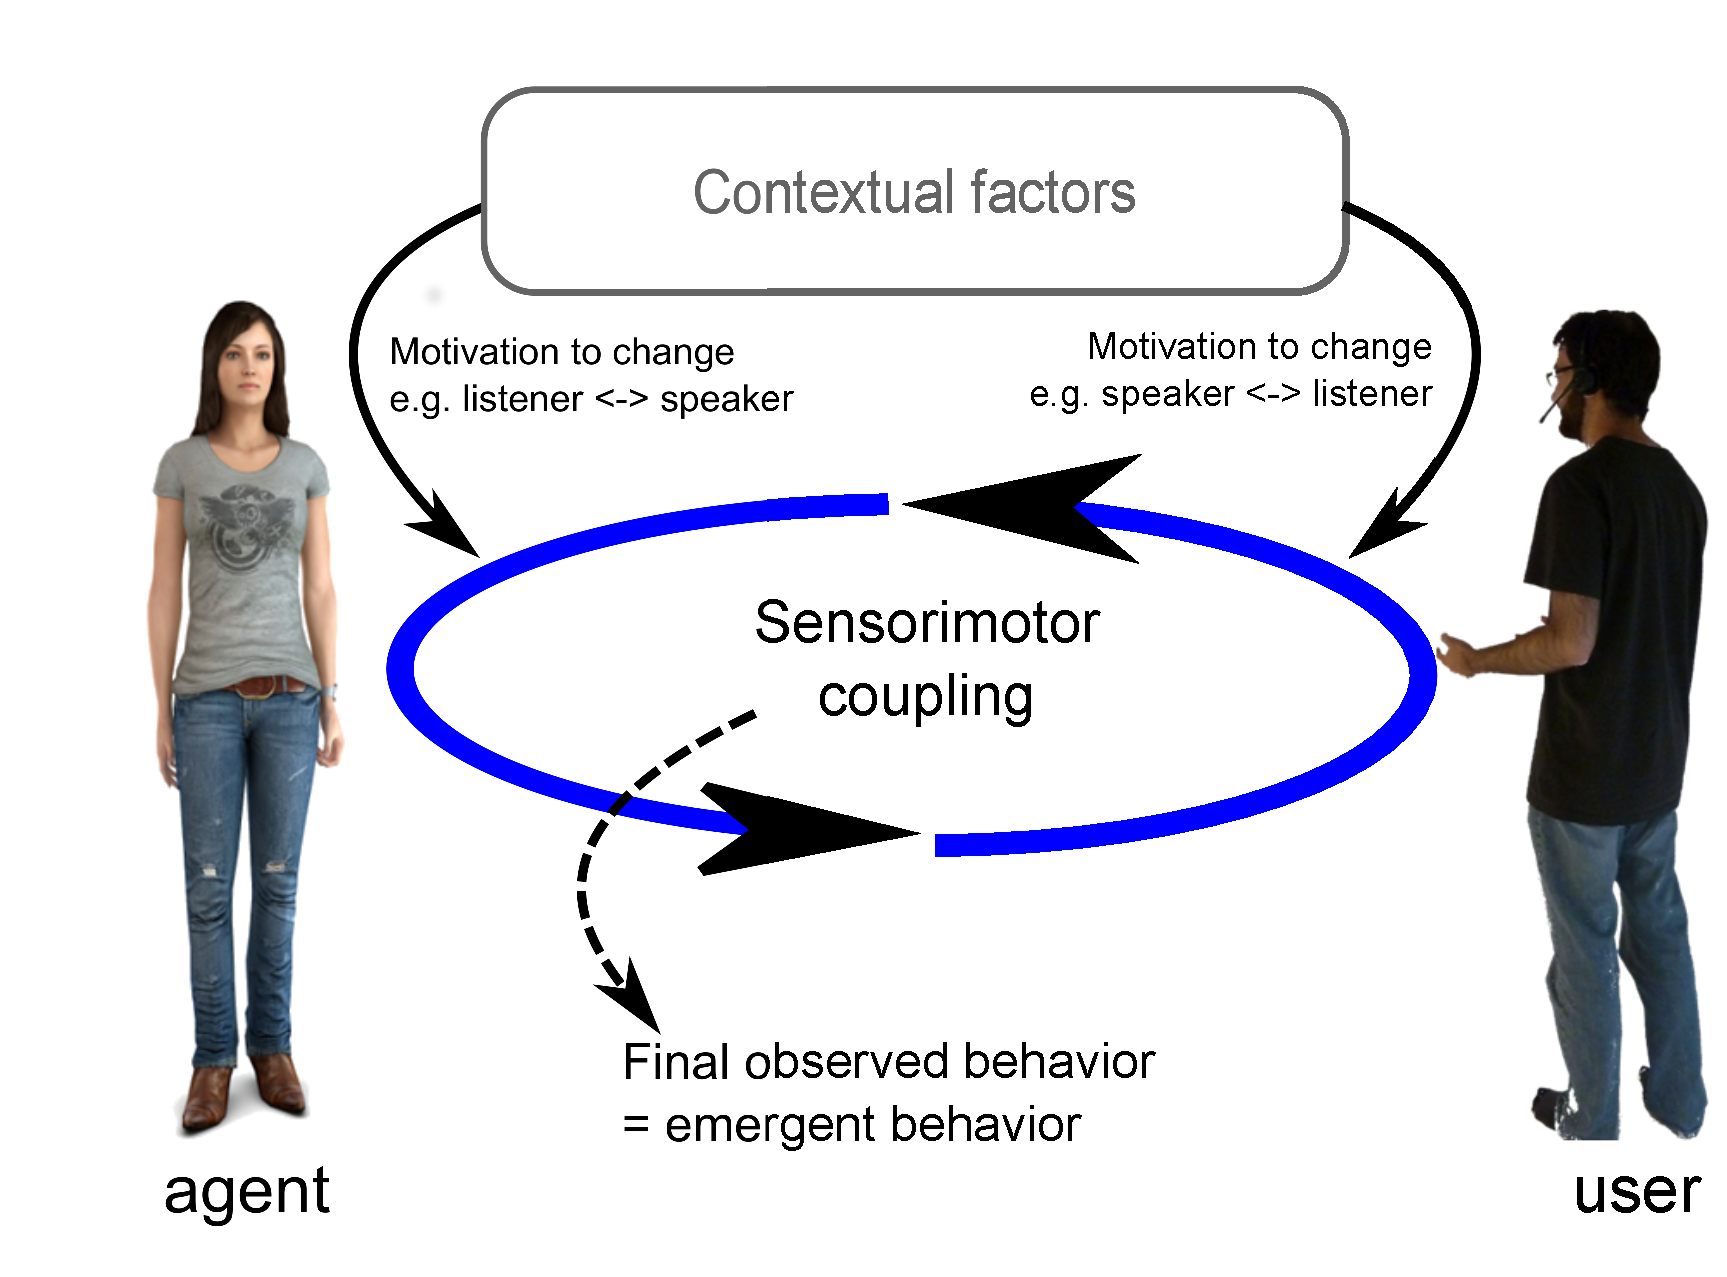
\includegraphics[width=\linewidth]{figure/schema_motivation.eps}

  \caption{The two levels of dynamics involved in the turn-taking management. 
    Top level: the contextual factors, like the verbal productions, and the interpersonal attitudes, vary the motivation the each agent has in the current situation to change its role (being the speaker or the listener). 
Bottom level: the coordination process itself, partly driven by the agent's motivation and partly resulting from the sensorimotor coupling between the two participants. 
The observed behavior of the agents is an emergent property resulting from the interplay of the agents' behavior.}
  \label{fig:mot}
\end{figure}
% the Distinction between the motivation to speak driven by contextual factors like verbal content, and interpersonal attitudes, and the coordination process itself partly driven by the motivation of the participants and emergent from the sensorimotor coupling between participants.}

The first level at the top of the figure represents the contextual factors that impact how the agents tries to take, release or keep the turn. These contextual factors are numerous. Examples of these variables are the nature of the verbal contribution, especially the importance the contribution has towards the progression of the dialog \citep{selfridge_bidding_2009}, its competitive or cooperative nature \citep{cafaro_effects_2016}, the agent's attitude towards its partner \citep{ter_maat_how_2010} or the agent's emotions \citep{ter_maat_turn_2009}.

These factors influence, or modulate, the ``motivation'' of the agent to claim the turn when it is the current listener or to release the turn when it is the current speaker. 
In other words, these factors define the relative strength of the goals of each agent, namely changing its role (speaker, listener) or still keeping it. It is worth noticing that this motivation continuously varies during the interaction. 
%In our model, these factors do not directly traduce into ``strategies" \citep{ter_maat_how_2010} or complete actions the agent will make towards the coordination of speaking turn but will more simply modulate the ``motivation'' the agent has to change its role (transitioning from speaker to listener or conversely). 
What we call here ``motivation" is similar to what other authors have called ``urge to speak" \citep{thorisson_multiparty_2010} or ``intentions"  to speak \citep{lessmann_towards_2004}, in the sense that it represents a variable that modulates the strength with which the agent will try to take or release the turn. We chose to call it ``motivation'' to remain as neutral as possible towards the contextual factors that could modulate this variable, as for example, taking the turn early is not always related to an urgency to say something, and is not always related to explicit communicative intentions, as participant's emotions and attitudes can also impact the agent's behavior. 

In the  model, this motivation is a variable that continuously varies between $-1$ and $1$. 
$-1$ means that the agent has a strong motivation to keep its current role (listening or speaking), while
$1$ means that the agent has a strong motivation to adopt the opposite role. 
%Between these two values the agent can continuously vary the strength with which it will try to keep or change its role, 
The closer the value of the motivation to $0$ the weaker the strength of the participant to change its role or to keep it. 

The value of the motivation influences, but does not solely determine, the final behavior of the agent in terms of taking, yielding or keeping the turn. The motivation variable represents the goal of the agent towards turn-taking, but the final behavior of the agent is an emergent property of the interaction between the agent and its partner. 
This principle results from the second loop of interaction in Figure \ref{fig:mot}. 
In this loop, the agent begins to vary its own signals regarding turn-taking (for example, decreasing loudness or pitch or gaze towards the user) based on its own goal as conveyed by the motivation variable. Nevertheless, the agent is coupled with its partner, and the signal production of its interlocutor directly influences the way it will vary its own signals.
Conversely the variation of its own actions will influence the behavior of its partner. 
As a result, the final behavior of the agent
%, either the participant will take, yield or keep the turn and the shape of this behavior 
is an emergent property of the interaction between the participants.
It results from the complex interplay between the own motivation of the participant and the cues given by its interlocutor.

\subsection{Scope of the modelling}

The objective of this study is the modeling of the continuous sensorimotor coupling between the participants. In this context, the motivation of the agent acts as a control parameter of the dynamics of this coupling. Thus the law of control of this motivation is out of the scope of this work.
%In our model, we suppose that the motivation value is influenced by different contextual variables as presented here, but we only interested for the moment in the modeling
Moreover, our aim here is not to define the law of control for the production of the verbal and nonverbal signals, as observed in human conversations, but to model the general dynamics of the behavior and thus to capture the way these various signals shape the agent's behavior. For the sake of generality, in the presentation of the theoretical model, we consider abstract values of these signals and their variations are simplified in purpose, compared to what can be observed in human conversations.
%exactly the signals produced in human conversations, but to model the more general dynamics of the signals produced by participants. The signal values taken as example here are then theoretical and their evolution is voluntarily simplified compared to human conversations. 
For instance, the different prosodic features are treated as continuous variables, whereas is human conversations their dynamics are linked to the phonemes produced by the participants. More precisely, the model accounts for the suprasegmental evolution of the prosodic signals, which is primarily linked to the coordination of turns.
% that's why we chose to abstract here from the part of the prosody that is correlated with the verbal content of what the user says. 
The same principle is followed for other signals mentioned in this article like gestures or gaze directions. 
Another reason for this abstraction % of the signals perceived and produced by the model is that our goal is to create a generic
is to make the  theoretical model independent to the actual sensors and actuators that could be used for real-time interactions between the agent and the user. 
We will see in section \ref{impl} the capacity of our implementation to adapt to real interactive setup, and will explain more in details how we used our theoretical values to modulate the prosody of the text-to-speech system.

\subsection{Components of the theoretical model}

We will now introduce in details our theoretical model, which is divided in two components as shown in Figure \ref{fig:mod-comp}: one in charge of the continuous perception of the user's behavior and one that controls the production of the different communicative signals. 

\begin{figure}
  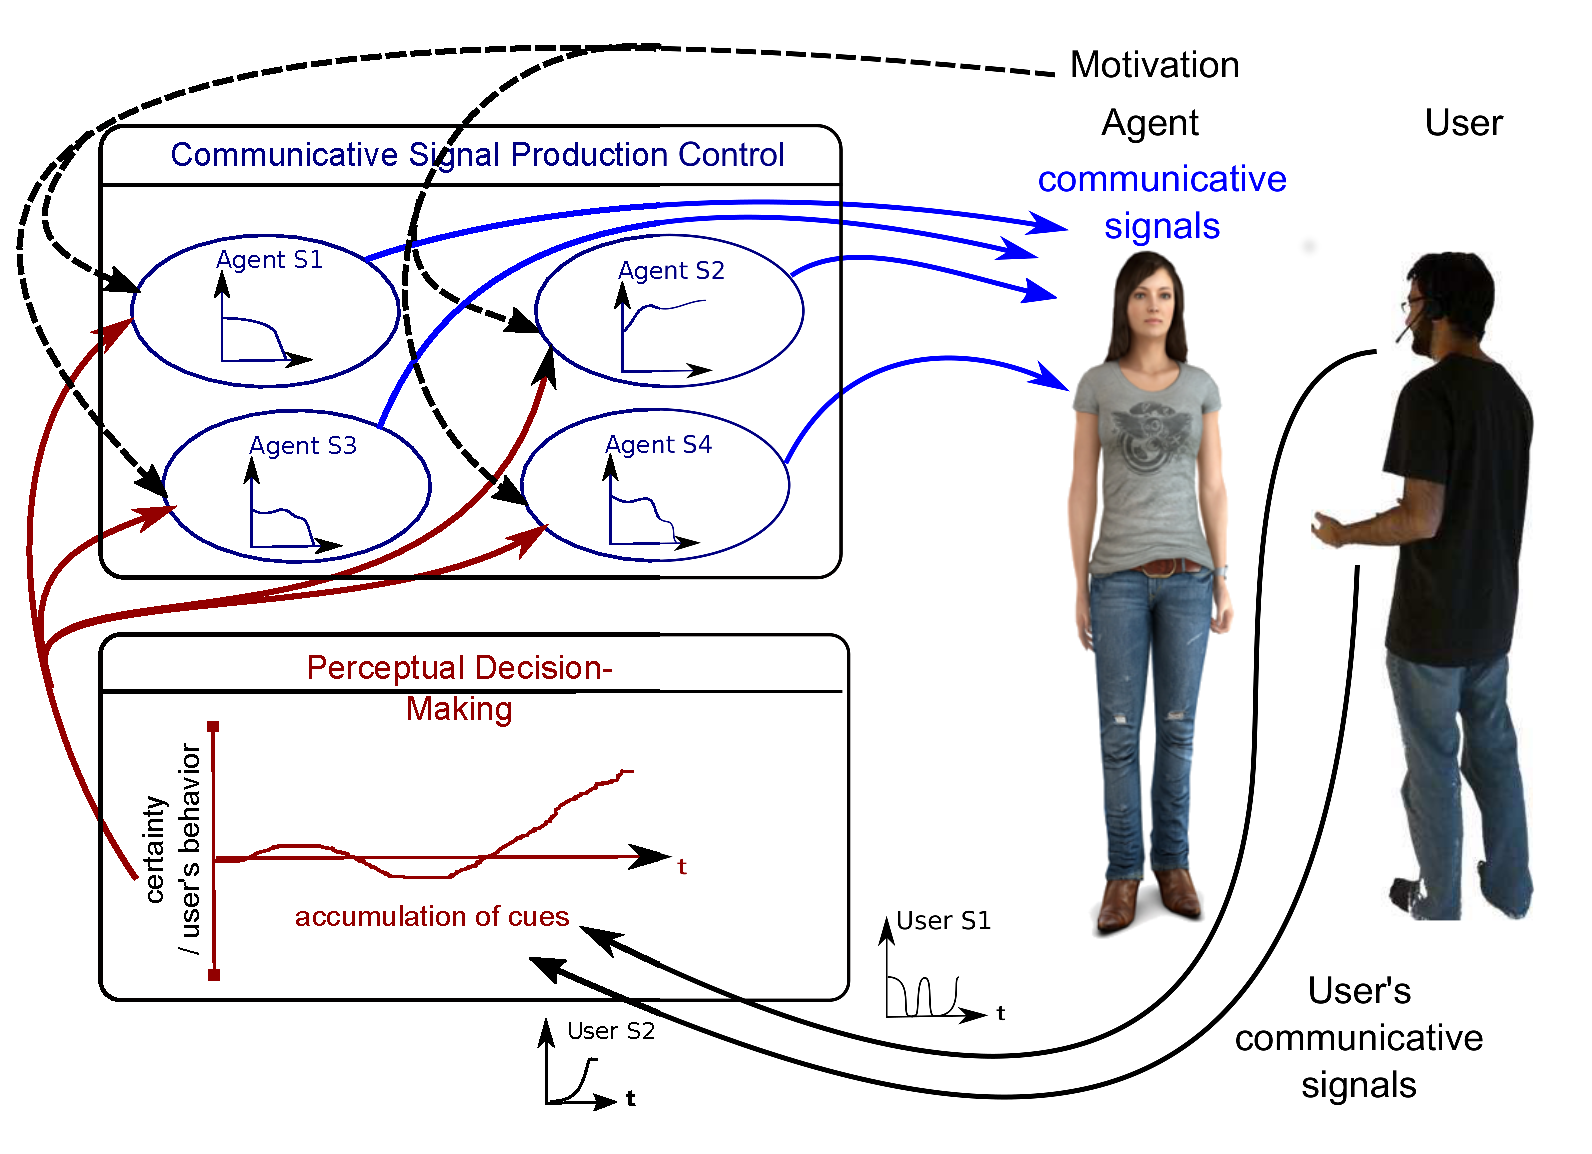
\includegraphics[width=\linewidth]{figure/modele_conceptuel_act.eps}
  \caption{Overview of Components of the theoretical model.}
  \label{fig:mod-comp}
\end{figure}

%First the agent tries to perceive the current behavior of the user between two alternatives, whether the user is changing role or not that is to say, whether the user is taking the turn or listening, if the agent is the current speaker or either the user is yielding or not the turn if the agent is the current listener. The agent continuously perceives the variations of the user signals over time, and continuously updates an accumulation variable that represents the degree of certainty the agent has about the user's behavior. 
%Second, the agent continuously modulates his nonverbal signals, based on the accumulation variable computed in the user behavior perception component and the agent's own motivation to change role. The way the agent controls his nonverbal signals is defined by a set of deterministic differential equations, where both accumulation and motivation are used to compute the attractors of the equations, that is, the final value towards which converge the agent signals.  

%We will now present more in details the different components of our model.

\subsubsection{Perceptual decision-making}
%\subsubsection{User behavior perception}

This component accounts for the dynamics of the decision-making. The underlying cognitive process is a perceptual decision-making task. The agent continuously perceives the variations of the signals produced by the user during the interaction, and continuously evaluates its certainty about the willingness of the user to be the next speaker (or listener). This degree of certainty is represented by an accumulation variable (see Figure \ref{fig:mod-comp}).
The user behavior perception component follows the paradigm of Two Alternative Forced Choice tasks (TAFC), for which different solutions have been proposed in order to model the timing of the decision making process (see \citep{bogacz_physics_2006} for a review). 
The Drift Diffusion Model (DDM) has shown its ability to predict the time required by a human subject to accurately discriminate the nature of the information it can perceive for a lot of tasks requiring perceptual decision-making. 
Interestingly the DDM have been used both in settings where the stimuli presented to the subject remained the same over the course of the decision-making process and settings where the stimuli varied \cite{ratcliff_note_1980}. This model conceptualizes the dynamics of the agent's decision-making as a stochastic process driven by the following equation:

\begin{equation}
  \frac{d\gamma(t)}{dt}=\alpha(t)+c\times\frac{dW}{dt}
  \label{perc_int}
\end{equation}

In our model, Equation \ref{perc_int}, $\gamma(t)$ represents the current degree of certainty the agent has about the behavior of its partner, $\alpha(t)$ an accumulation rate that varies depending on the continuous variations of the user's signals and $c\times\frac{dW}{dt}$ representing a noise in the perception process of the participants as defined by the DDM. The decision making process is therefore continuously driven by the perception of the signals produced by the agent's partner.

%Depending on 
The sign of $\gamma(t)$ indicates that the agent is tending to adopt one alternative or the other. 
When $\gamma(t)>0$, the higher its value, the more the agent is certain about its partner's willingness to switch to the opposite role.
When $\gamma(t)<0$, a high absolute value means that the agent is very certain that its partner actually wants to keep its current role. 

The ongoing decision-making process ends when $\gamma(t)$ crosses a threshold $\theta_{\gamma}^{\pm}$. $\gamma(t)$ is then set to 0 and a new decision making process starts.
$\gamma(t) \geq \theta_{\gamma}^{+}$ means that the agent is certain that its partner has switch to the opposite role and the agent changes its behavior accordingly (defined by the component responsible for the control of signals). $\gamma(t) \leq \theta_{\gamma}^{-}$ means that the signals it can perceive indicate that its partner wants to keep its current role. 
%When $\gamma(t)>0$, the agent is more or less certain about the fact that its partner wants to change role, that is, if the partner is giving or yielding the turn. When  $\gamma(t)<0$, the agent is more or less certain about the fact that its partner wants to change role. 

%When $\gamma(t)$ crosses a threshold $\theta_{\gamma}^{\pm}$, favoring one or the other alternative, it means that the agent becomes certain about the nature of the behavior of its partner, either the partner changes role $\theta_{\gamma}^{+}$ or keep its current role $\theta_{\gamma}^{-}$. When the accumulation value crosses the threshold $\theta_{\gamma}^{+}$, the agent changes its own role. As a consequence, the agent activates the corresponding behavior (defined by the component responsible for the control of signals) and initialize a new perceptual decision-making task, corresponding to its newly adopted role.
%as  modifying the equations controlling its nonverbal signals and the user behavior perception equation. 

%On the opposite, when $\gamma(t)$ crosses the threshold $\theta_{\gamma}^{-}$, the agent resets its accumulation value, forgetting what it has perceived before and beginning a new perceptual decision-making process. 
We will see in section \ref{mod_analysis}, that reinitializing this accumulation value allows, for instance, the agent motivated to take or to yield the turn to try to initiate a new turn transition if the previous try did not succeed. 
It occurs when its partner does not respond to its turn-yielding signals by taking the turn, or when the agent's partner being the current speaker, prevents the agent to take the turn.

To account for the sensorimotor coupling between the two agents, we made the accumulation rate $\alpha(t)$ being a function of the variations of the signals produced by the agent's partner. This function has a general shape defined by the equation: 

\begin{equation}
  \alpha(t) = \sum_{j=0}^{n_{s}} \alpha_{j}(\dot{s}_j(t),s_j(t))
  \label{alpha_func}
\end{equation}

Equation \ref{alpha_func} means that $\alpha(t)$ continuously varies according to a sum of partial accumulation processes $\alpha_{j}$ that compute an accumulation rate for each signal $s_j$ the agent can perceive ($n_s$ denotes the number of signals). %of the agent's partner. 
$\alpha_{j}>0$ indicates that the current variations in the signals produced by its partner are in favor of the assumption that the partner is switching to  the opposite role.
$\alpha_{j}<0$  means that the perceived variations of the signals are in favor of the assumption that the partner is keeping its current role. 
%$n_{s}$ represents the number of signals of the user. 

\paragraph{Illustrative simulation S1.}% To illustrate the  perceptual decision-making process, 
Let's consider a situation with an agent able to perceive the variations of loudness, pitch, and gaze direction of the user, three cues that are considered as used by participants to coordinate their turns (see section \ref{backgd}). 
%For gesture, we refer to gesticulations as defined by \citep{duncan_signals_1972} as the production of gestures without referring to the meaning of these gesture. 
% TODO
In this simulated interaction, the agent was the current speaker and the user the current listener. The behavior of the user was here simulated.
%The user is initiating some gesticulations, slowly increasing their speed over time, then 
The user averted its gaze after 750~ms and started to speak at $t=1~s$. %take the turn at about 1~s. 
Figures \ref{fig-volume-user1}, \ref{fig-pitch-user1} and \ref{fig-gaze-user1} illustrate the variations of the simulated user's signal production, as perceived by the agent. 
%varies his signals as presented in figure \ref{part_actions}. It represents a user beginning to initiate gesticulations 
Figure \ref{acc_example} illustrates the resulting dynamics of the perceptual decision-making process. 
%In this scenario, the agent is the current speaker and a simulated user tries to take the turn by varying its signals according to figure \ref{part_actions}. 
The curve at the top is the evolution of the accumulation rate over time, $\alpha(t)$ and the curve at the bottom the evolution of the accumulation value $\gamma(t)$. In these scenarios, the second term $c \times \frac{dW}{dt}$ has been set to 0 that the accumulation process in this example has no noise. 

% TODO: subfigures

% \begin{figure}
% \centering
% \includegraphics[width=\linewidth]{figure/Gesticulation_speed_partenaire.pdf}
% \caption{Gesture production speed of the simulated user.}
% \label{part_gesture}
% \end{figure}

\begin{figure}
  \centering
  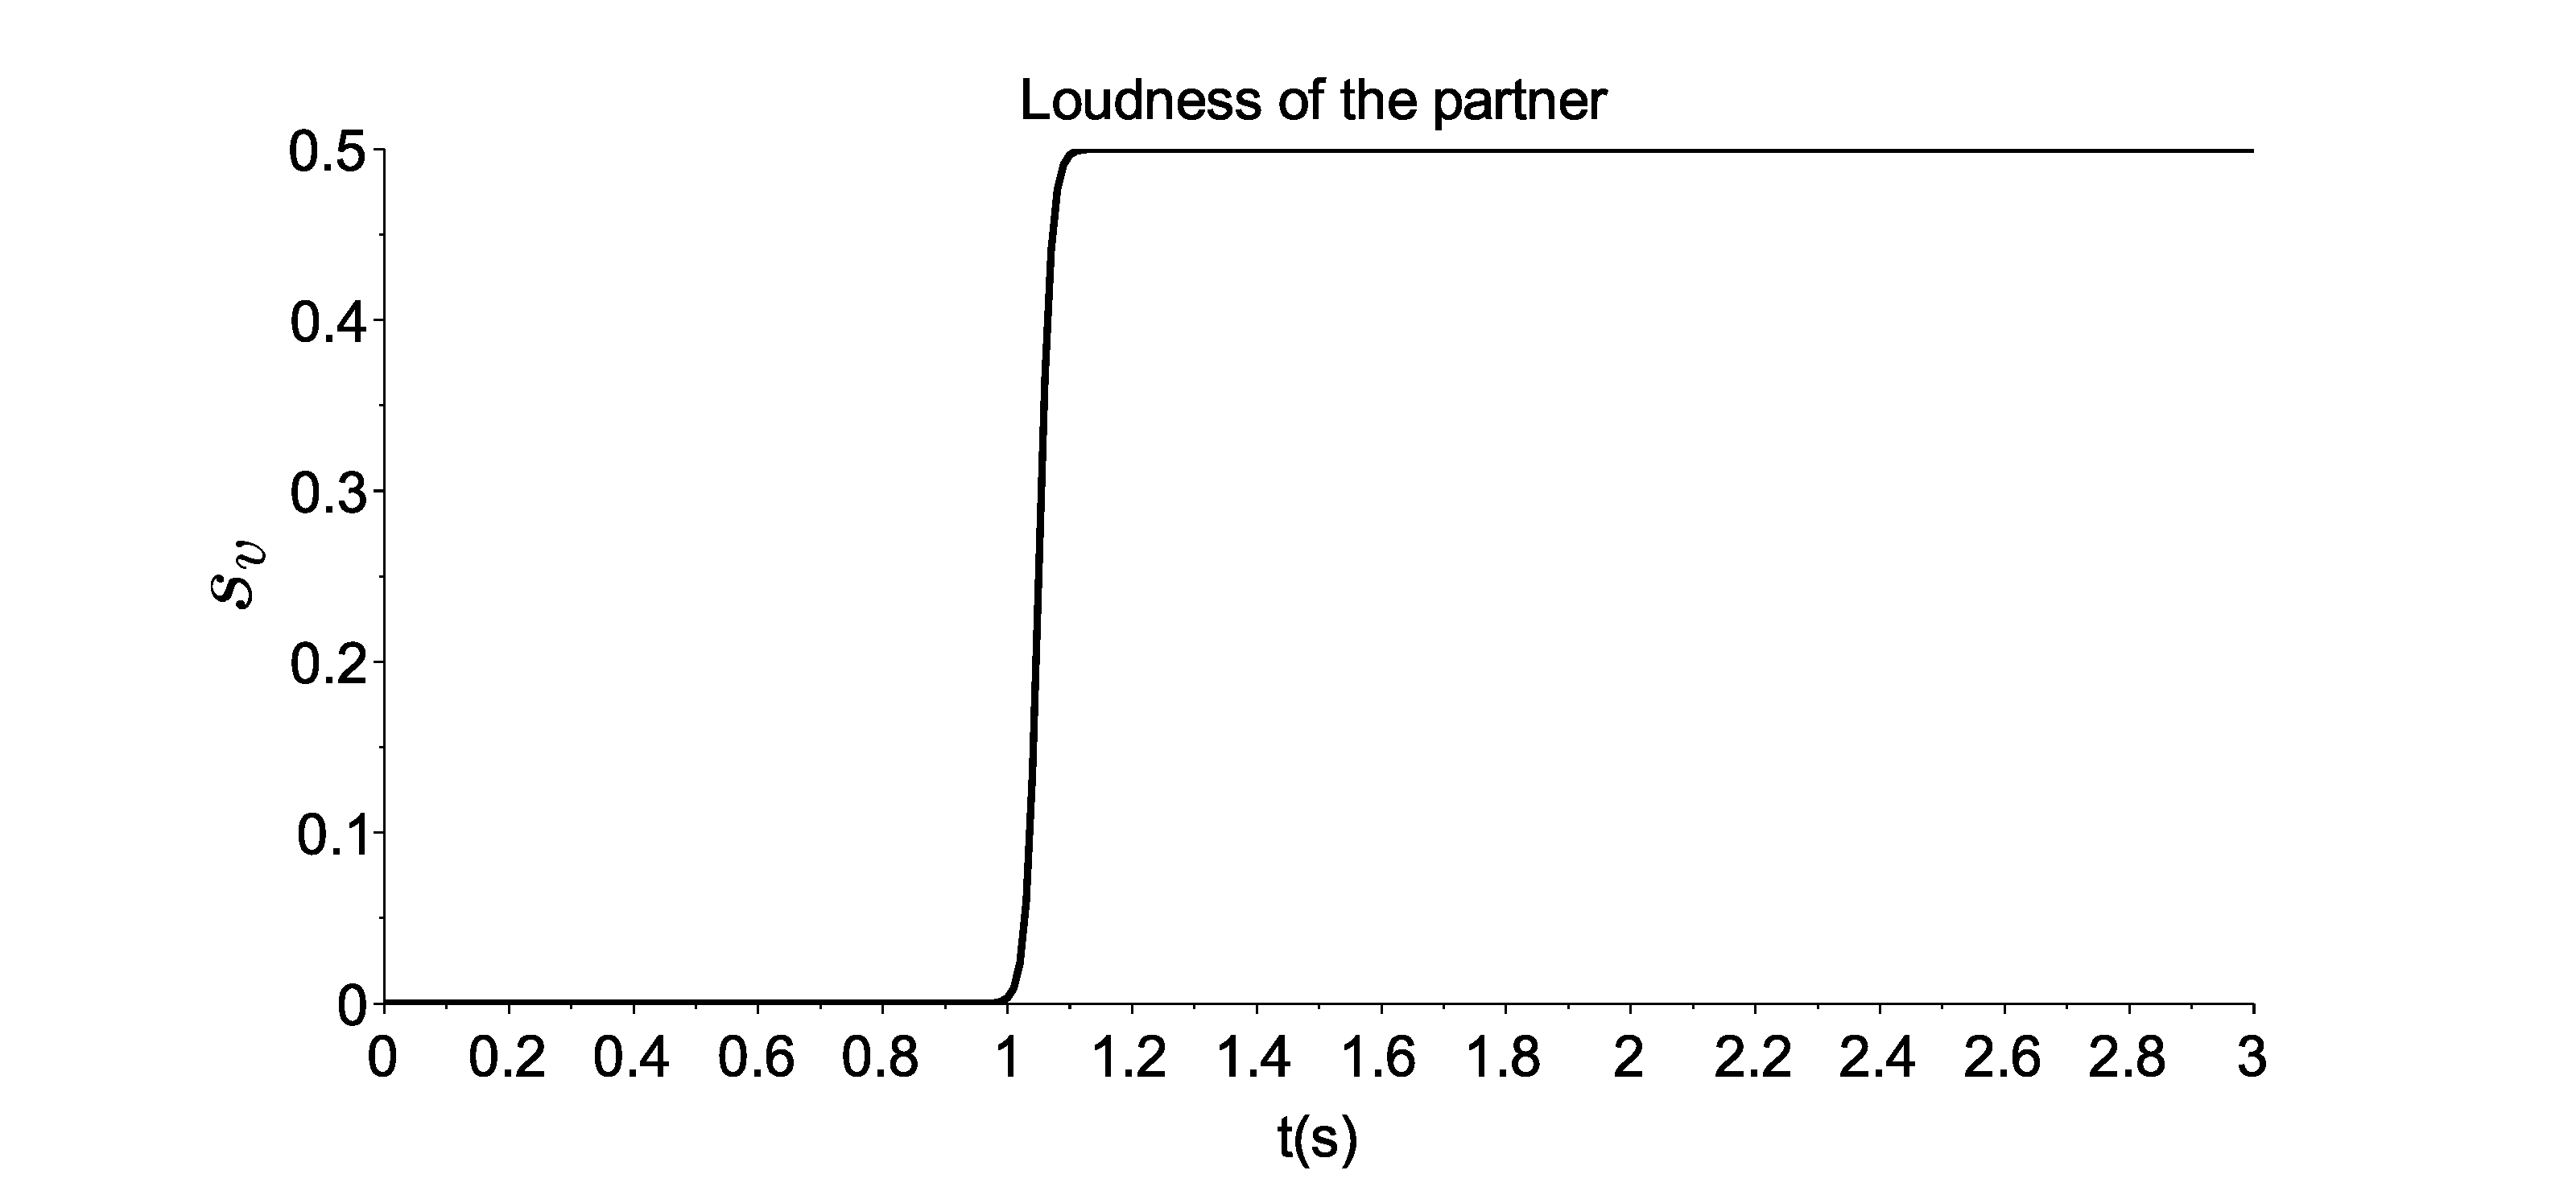
\includegraphics[width=\linewidth]{figure/loudness_simulated_partner.pdf}
  \caption{Illustrative simulation S1: variation of the voice loudness of the simulated user.}
  \label{fig-volume-user1}
\end{figure}

\begin{figure}%[b]
  \centering
  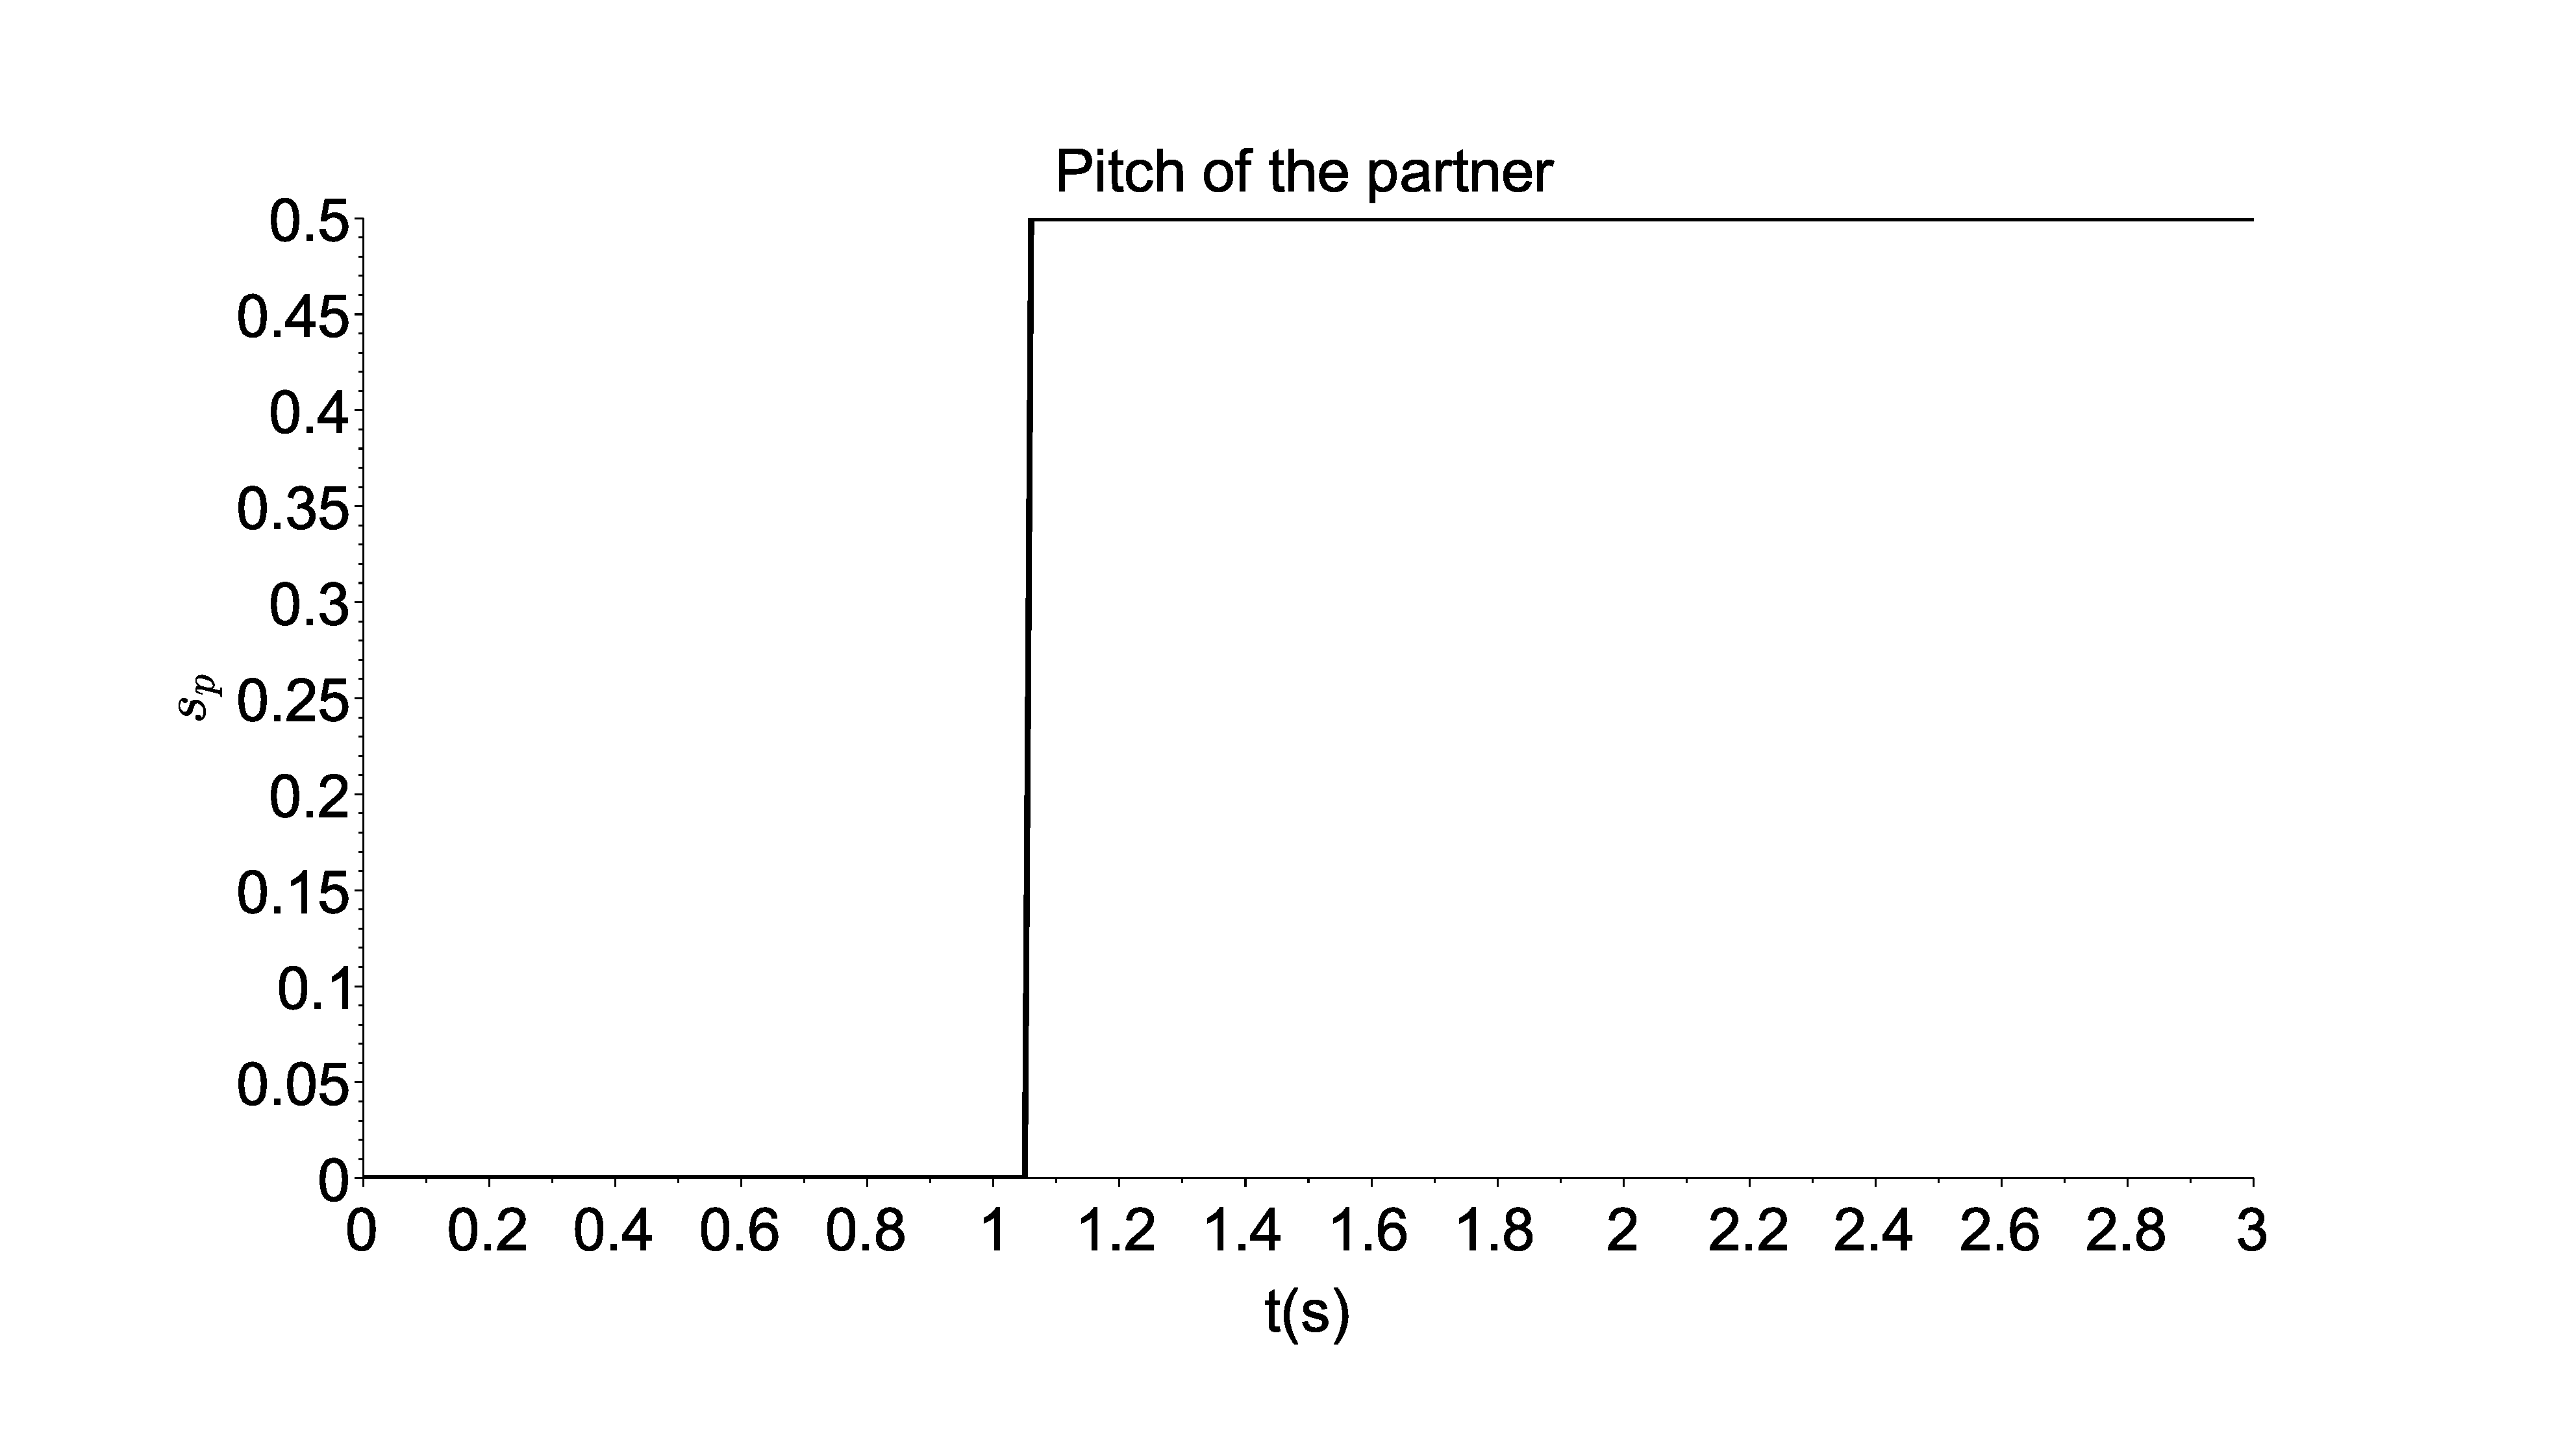
\includegraphics[width=\linewidth]{figure/Pitch_partenaire.pdf}
  \caption{Illustrative simulation S1: variation of the pitch of the simulated user.}
  \label{fig-pitch-user1}
\end{figure}

\begin{figure}
  \center
  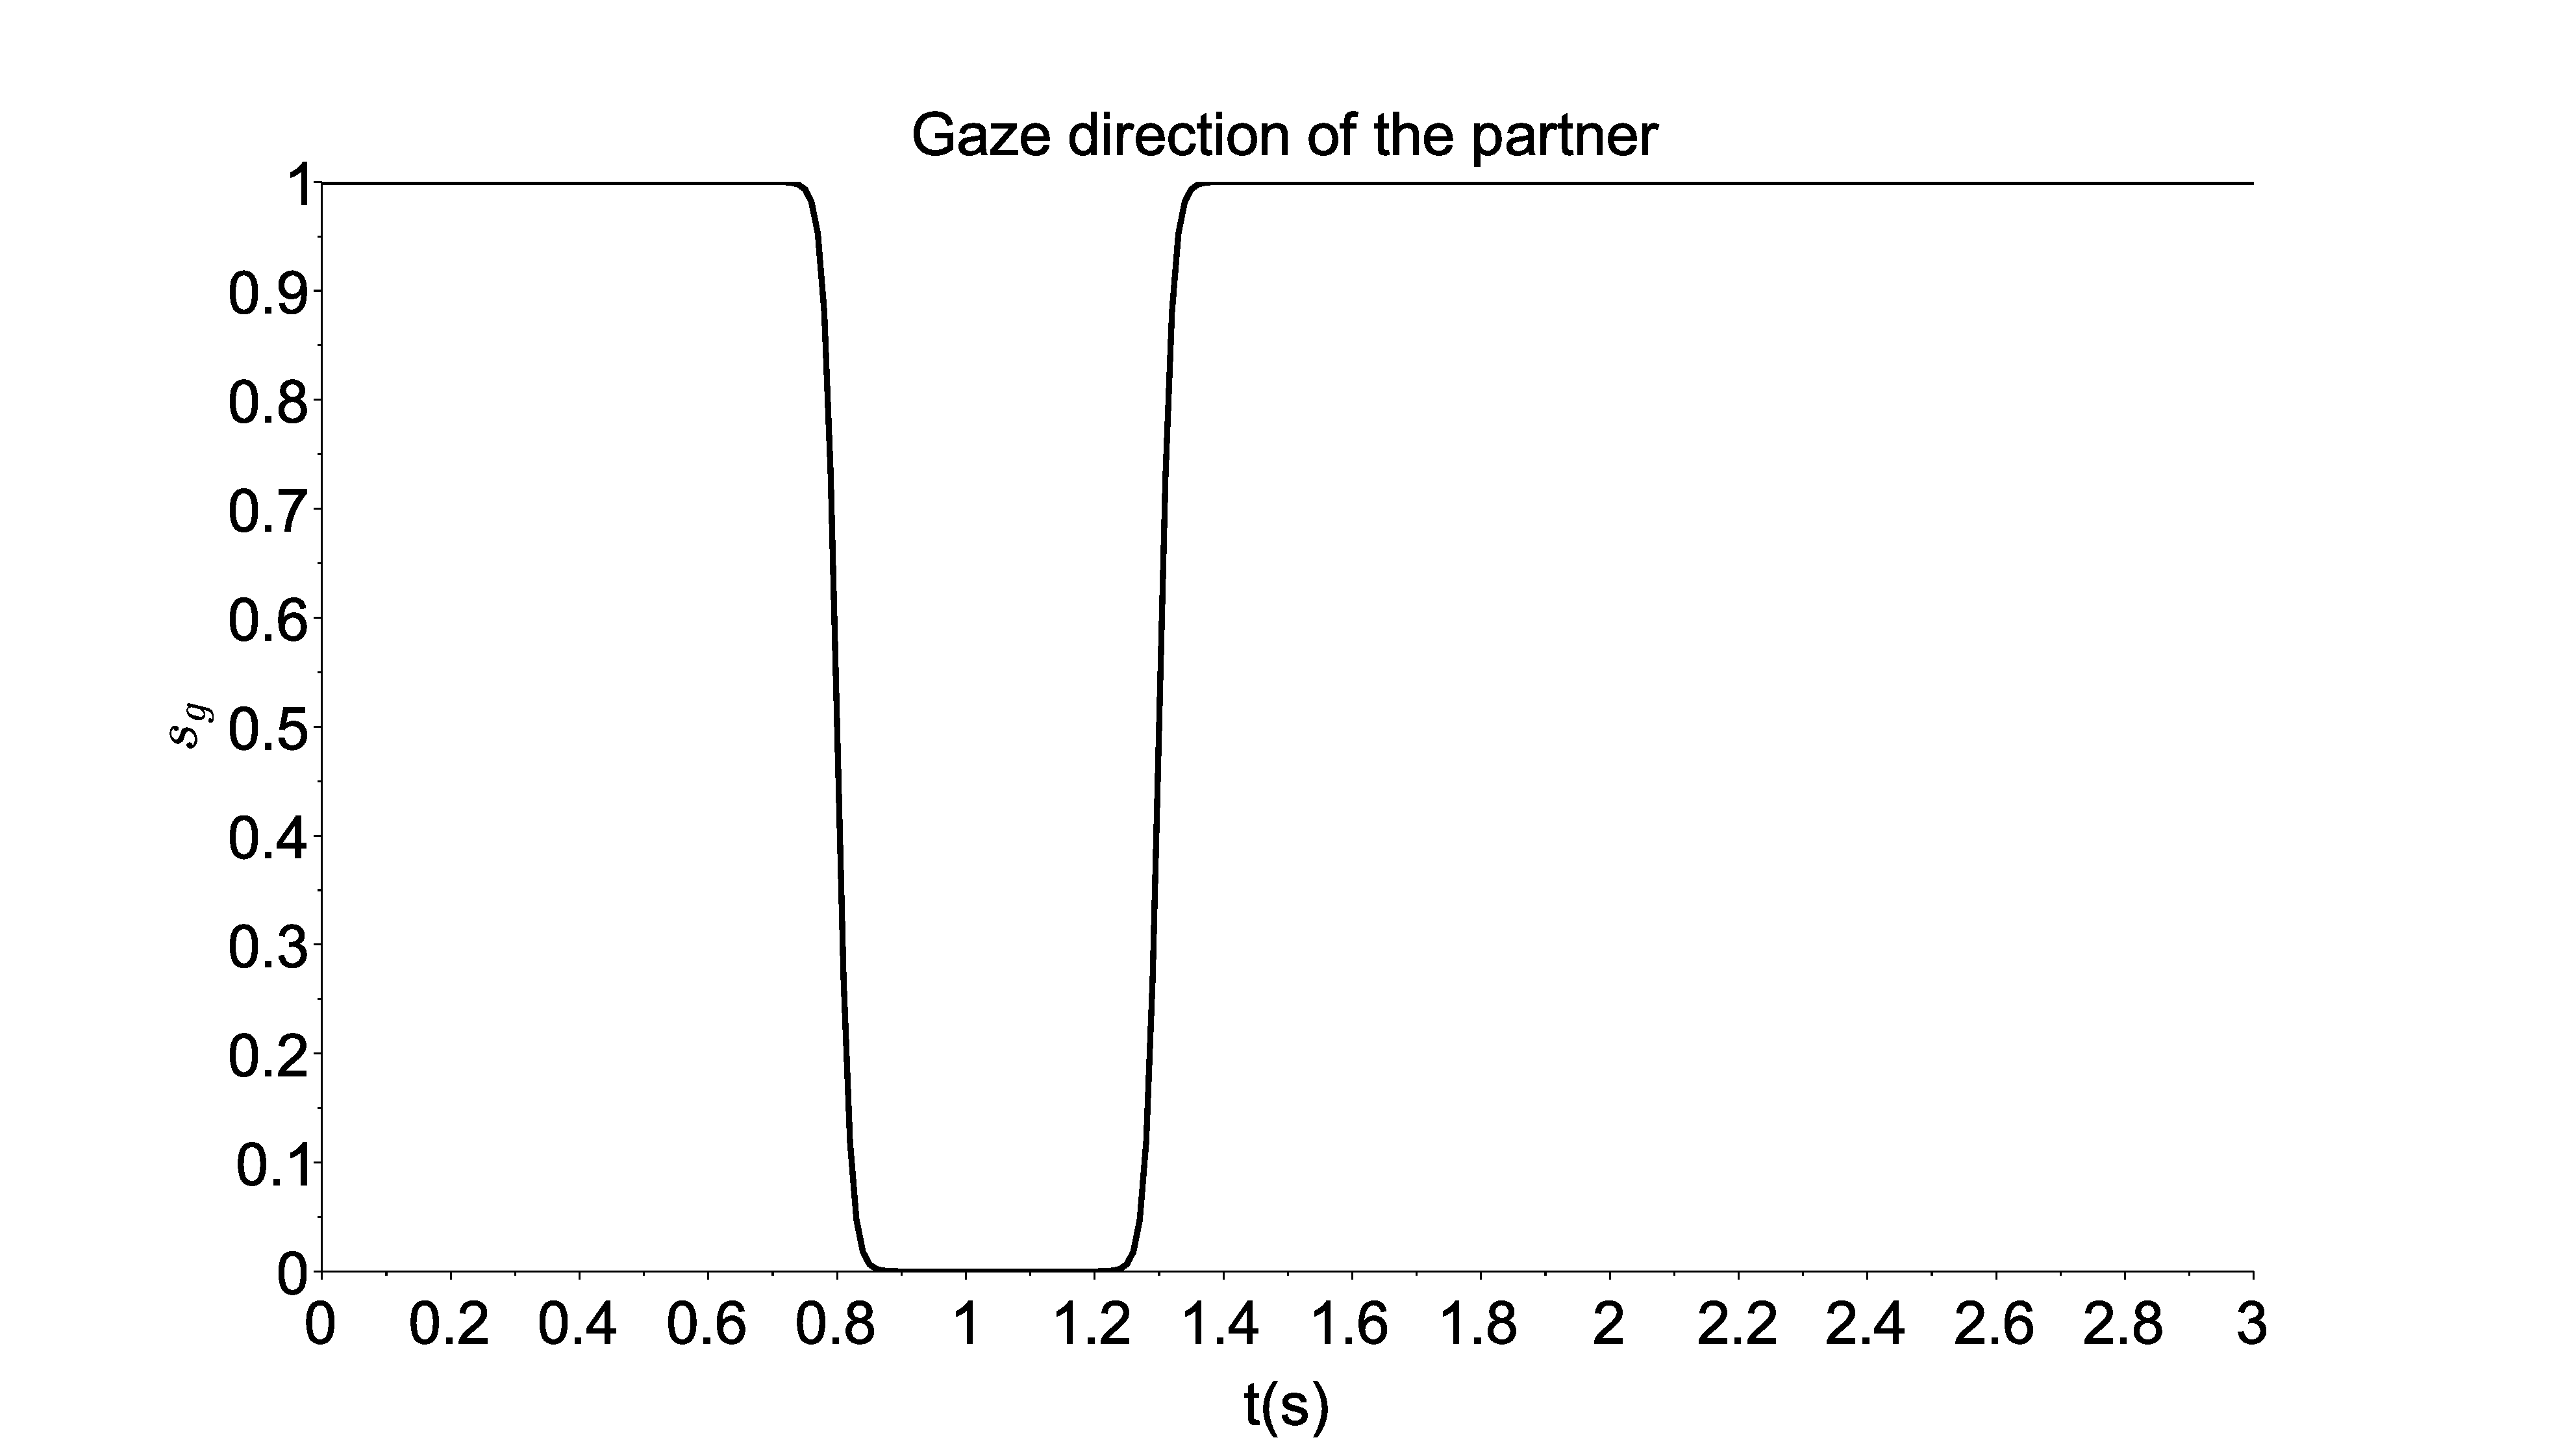
\includegraphics[width=\linewidth]{figure/Gaze_partenaire.pdf}
  % \end{subfigure}
  \caption{Illustrative simulation S1: variation of the gaze direction of the simulated user.}
  \label{fig-gaze-user1}
\end{figure}

\begin{figure}
  \centering
  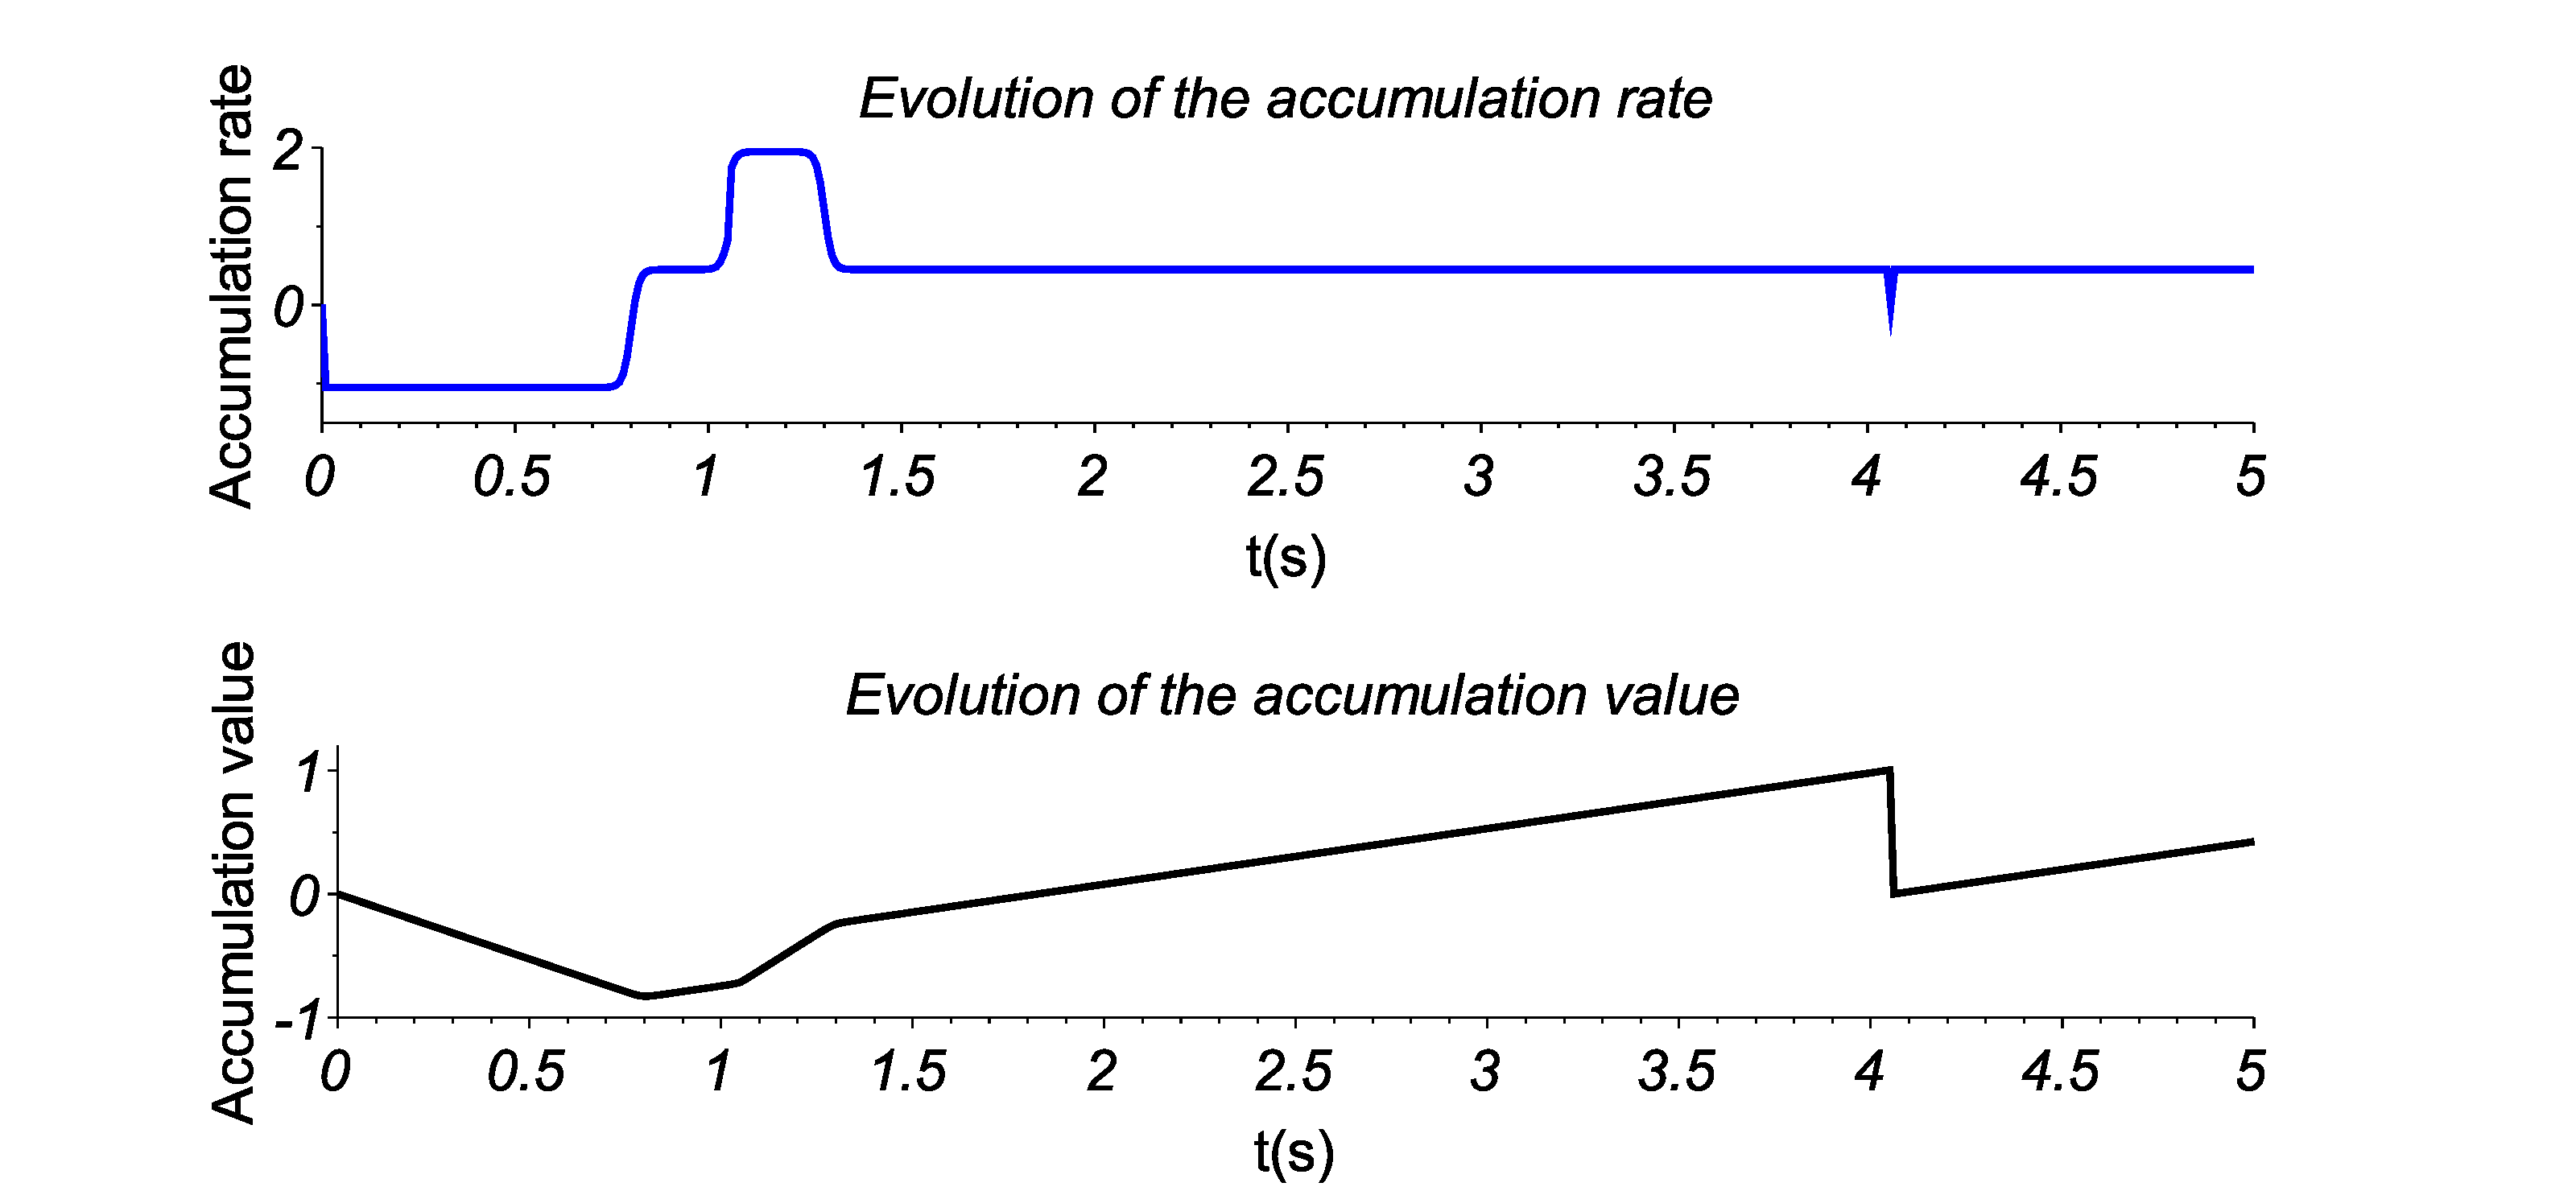
\includegraphics[width=\linewidth]{figure/illustration_ddm_speaker.pdf}
  \caption{Illustrative simulation S1: resulting dynamics of the perceptual decision-making process for the simulated speaker agent.}
  \label{acc_example}
\end{figure}

At the beginning of the scenario, the user did not produce any turn-taking signals, thus $\gamma(t)$ was decreasing, meaning that the agent was getting more and more confident about the user's intention to not claiming the turn. 

At $t=0.75~\text{s}$, the agent started to get some information about the user's willingness to take the turn (gaze aversion), thus the accumulation rate was positive. 
As soon as the user produced an additional turn-taking signal (starting to speak, resulting in a sudden increase in the pitch and volume of his voice), the accumulation rate raised to a higher value. 
After $=1.2~\text{s}$, the user's gaze direction led the agent to believe that the user did not want to become speaker, in contradiction with the information provided at the same time by the verbal channel (the user was actually speaking). Therefore the accumulation rate has fallen to an intermediate positive value. 
As a result, the agent accumulated information about the user's intention to effectively take the turn and $\gamma(t)$ reached the positive threshold ($\theta_{\gamma}^{+}=1$), leading it to be certain about the user's behavior. At this point ($t=4~\text{s}$), the agent made a definitive decision and it reset its perceptual decision-making process. 

% As the user only and slightly increases its gesture production at the beginning, the accumulation value decreases towards the negative threshold $\theta_{\gamma}^{-}=-1$. 
% Then, as the user increases its gesture production and look away from the agent after approximately 750 ms, the accumulation rate varies to a positive value, but close to $0$, that results in an accumulation value that slightly increases, after which the user begins to speak after 1.1s. This sudden variation of the prosody descriptors strongly increases the accumulation rate, then the accumulation value rapidly converges towards the value $\theta_{\gamma}^{+}=1$, meaning that the agent is certain that the user is taking the turn. 

The  difference in the dynamics of the perceptual decision-making process, before and after $t=1~\text{s}$, illustrates the principle of additivity of the perceptual decision-making process, captured by Equation \ref{alpha_func}: the more signals the user produces
%The more the user produces signals,   
 the higher the accumulation rate and the faster the agent detects that the user is taking the turn. This additivity of the perceptual process has been reported for human conversations \citep{gravano_turn-taking_2011,hjalmarsson_additive_2011}. 

\subsubsection{Production of the communicative signals}

The second component of our theoretical model controls the continuous production of the verbal and nonverbal signals of the agent.
Following the principles of the behavioral dynamics formulated by \citep{warren_dynamics_2006}, each signal produced by the agent is controlled by a differential equation, representing the law of control of the agent's behavior. These equations have the following general shape: 

\begin{equation}
  \ddot{a_j}(t)= -b\times\dot{a_j}(t) - k_g \times(a_j(t) - f(m(t),\gamma(t)))
  \label{signal_control}
\end{equation}

$a_j(t)$ representing the current value of signal $j$, ($\ddot{a_j}(t)$ being the second derivative of the signal), $-b$ a damping term representing the intrinsic inertia of the agent to vary its signals, and $k_g\times(a_j(t)-f(m,\gamma))$ defining the value towards which the agent's signal is converging. In our theoretical model, each signal variable $a_j(t)$ is normalized within $ [0.0,1.0] $, $0.0$ representing the minimal value of the signal (no-signal or baseline), and $1.0$ the maximal value of the signal. The way these theoretical values are translated into realistic physical values depends on the nature of the signal and on the actuator used to execute the action corresponding to the signal produced. 
$k_g$ represents a stiffness parameter of the equation, the greater the value of $k_g$ the more the participant will rapidly vary its signal towards the final value of the equation. 
$f(m,\gamma)$ is a function that defines the attractor of the system. As presented at the end of section \ref{backgd}, the modulation of each signal is directly influenced by the motivation of the agent, $m$, and the accumulation value $\gamma$ provided by the perceptual decision-making component of our model.

%As an example showing how these equations are used to modulate the signals of the agent, 
\paragraph{Illustrative simulation S2.} Let's consider an agent currently being the speaker and modulating two prosodic signals ($v$ = loudness, $p$ = pitch) and its gaze direction, $g$. 
Like for the previous example, these variations are here theoretical.
The aim was not here to reproduce exactly the variations of the signal observed during human conversations, but to capture the dynamics of the signal productions, for instance that loudness and pitch tend to increase %and the speech rate to decrease 
during conflicting overlaps between partners, or to decrease during ends of turn. 

For each signal $j \in \lbrace p,v,g \rbrace$ produced by the agent, being the current speaker, we defined the following different equations $f_{j_{loc}}(m,\gamma)$, used in Equation \ref{signal_control}.
%According to Equation \ref{signal_control}, $f_p, f_v$ and $f_r$ are 
These functions control dynamically the value toward which each signal is varying at a given instant of time.

% Here are the new equations
\begin{equation}
\begin{array}{lcl}
f_{p_{loc}} & = &  \frac{1}{2}\Big( 1 - S(\gamma) \big( \gamma m S(-m) - S(m+\gamma)S(m) \big) \Big)
%0.5 -0.5 \times \gamma \times m \times S(-m) \times S(\gamma) - 0.5 S(m+\gamma) \times S(\gamma) \times S(m)\\
 %& = & \frac{1}{2}(1 - S(\gamma)\times\gamma \times m \times S(-m) - S(m+\gamma) \times S(m)))
\end{array}
\label{eq_speaker_pitch}
\end{equation}

\begin{equation}
f_{v_{loc}} = f_{p_{loc}}
\label{eq_speaker_volume}
\end{equation}

\begin{equation}
\begin{array}{lcl}
f_{g_{loc}}&=& \frac{1}{2}\Big( 1+\gamma m S(\gamma) \big(S(m) - S(-m)\big) \Big)\\
%& & 0.5 +0.5\times \gamma \times m \times S(\gamma) \times S(m) \\
%& & -0.5 \times \gamma \times m \times \times S(\gamma) \times S(-m) \\
%&=& \frac{1}{2}((1+\gamma \times m \times S(m) \times (S(\gamma) - \gamma \times m \times S(\gamma) \times S(-m))\\
\end{array}
\label{eq_speaker_gaze}
\end{equation}

\begin{equation}
S(x) = \frac{1}{1+e^{-10x}}
\label{eq_sigmoid}
\end{equation}

% \begin{equation}
% \left\lbrace
% \begin{array}{l c l}
% f_p(m(t),\gamma(t)) &=& \frac{1}{2}(1+S(\gamma(t))(S(-m(t)) - S(m(t)))\\
% f_v(m(t),\gamma(t)) &=& f_p(m(t),\gamma(t))\\
% f_r(m(t),\gamma(t))& =& \frac{1}{2}(1- S(\gamma(t)) \\
% S(x)&=&\frac{1}{1+e^{-5x}}
% \end{array}\right.
% \label{attr_foncs}
% \end{equation}

%$(m(t),\gamma(t))$ being the function defining how the final value of the pitch varies, 
%$f_v(m(t),\gamma(t))$ being the function defining how the final value of the loudness of the participant's voice varies
%and $f_r(m(t),\gamma(t))$ defining the variation of the final value of the speech rate. 

In these equations, we used the sigmoid function $S$ (Equation \ref{eq_sigmoid}) that permits to set to $0$ some terms, depending on the value of $\gamma(t)$ or $m(t)$ (when $x \gg 0$, $S(x)\approx 1$ and when $x \ll 0$, $S(x)\approx 0$). 
%The three functions have a quit similar behavior. 
For example for the control of the pitch, 
when $m(t) \gg 0$, Equation \ref{eq_speaker_pitch} reduces to $f_{p_{loc}}(m,\gamma) \sim \frac{1}{2}\big( 1-S(\gamma) \big)$, 
when $m(t) \ll 0$, $f_{p_{loc}}(m,\gamma) \sim \frac{1}{2}\big( 1 + S(\gamma)\big)$ 
and when $\gamma(t) \ll 0$, $f_{p_{loc}}(m,\gamma) \sim \frac{1}{2}$. 
%when $m(t) \gg 0$, the equation reduces to $f_v(m(t),\gamma(t)) \sim \frac{1}{2}(1-S(\gamma(t)))$, 
%when $m(t) \ll 0$, it becomes $f_v(m(t),\gamma(t)) \sim \frac{1}{2}(1 + S(\gamma(t))$ 
%and when $\gamma(t) \ll 0$, the equation becomes $f_v(m(t),\gamma(t)) \sim 0.5$. 
% ----

We set these functions such as, when the current speaker has a strong motivation to keep on speaking ($m(t) \ll 0$) and has accumulated enough cues indicating that the current listener is about to take the turn  ($\gamma(t) \gg 0$), the agent is expected to increase the loudness and the pitch of its voice to avoid its partner to take the turn, resulting in a conflicting overlap. 
%In such a situation, we also expect the speech rate to decrease, as observed by \citep{schegloff_overlapping_2000}.
Otherwise, when the current speaker's current goal is to leave the turn ($m(t) \gg 0$), it is expected to lower its loudness and pitch, even faster if the listener is starting to speak (all the signals are falling to 0).
%We defined these different functions such as when $m(t)<0$ and $\gamma(t)>0$ the loudness and the pitch increase, representing a conflicting situation, and the speech rate decreases following the observations made by \citep{schegloff_overlapping_2000}. When $m(t)>0$ and $\gamma(t)>0$ the loudness, the pitch and the speech rate decrease until $0$. 
Notice that setting $f_p = f_v$ is an approximation that makes the two signals to follow the same dynamics, according to the signs of $m(t)$ and $\gamma(t)$. 

Because our approach assumes the sensory-motor coupling of the two interacting agents, we have here to simulate the dynamic of its partner's behavior, as perceived by the agent.
For the sake of simplicity, we simulated the dynamic of the perceptual decision making using the following equation: $\gamma(t)=1-2e^{-t}$. 
It means that in our simulated scenario, at the beginning the agent was certain that the listener is not claiming the turn ($\gamma(0) = -1$) and that the agent was rapidly accumulating some cues in the current listener's behavior indicating the willingness of the listener to take the turn. 

%Based on these equations, 
Figure \ref{demo_simu_l1} shows how the agent varied its prosodic signals when it was strongly motivated to keep on speaking ($m=1$).
As the accumulation $\gamma(t)$ increased, the resulting values of $f_v$ and $f_p$ increased towards $1$ and $f_g$ decreased towards $0$. 
Accordingly, the theoretical loudness and pitch of the agent raised to their maximum values (as expected during a conflicting overlap where the speaker tries to keep its role, and thus is modulating its signals production) in reaction to the listener's behavior that was trying to take turn. 

%We simulated a positive variation of the accumulation value from $-1$ to $1$ according to equation $\gamma(t)=1-2e^{-t}$. 

\begin{figure}
  \centering
  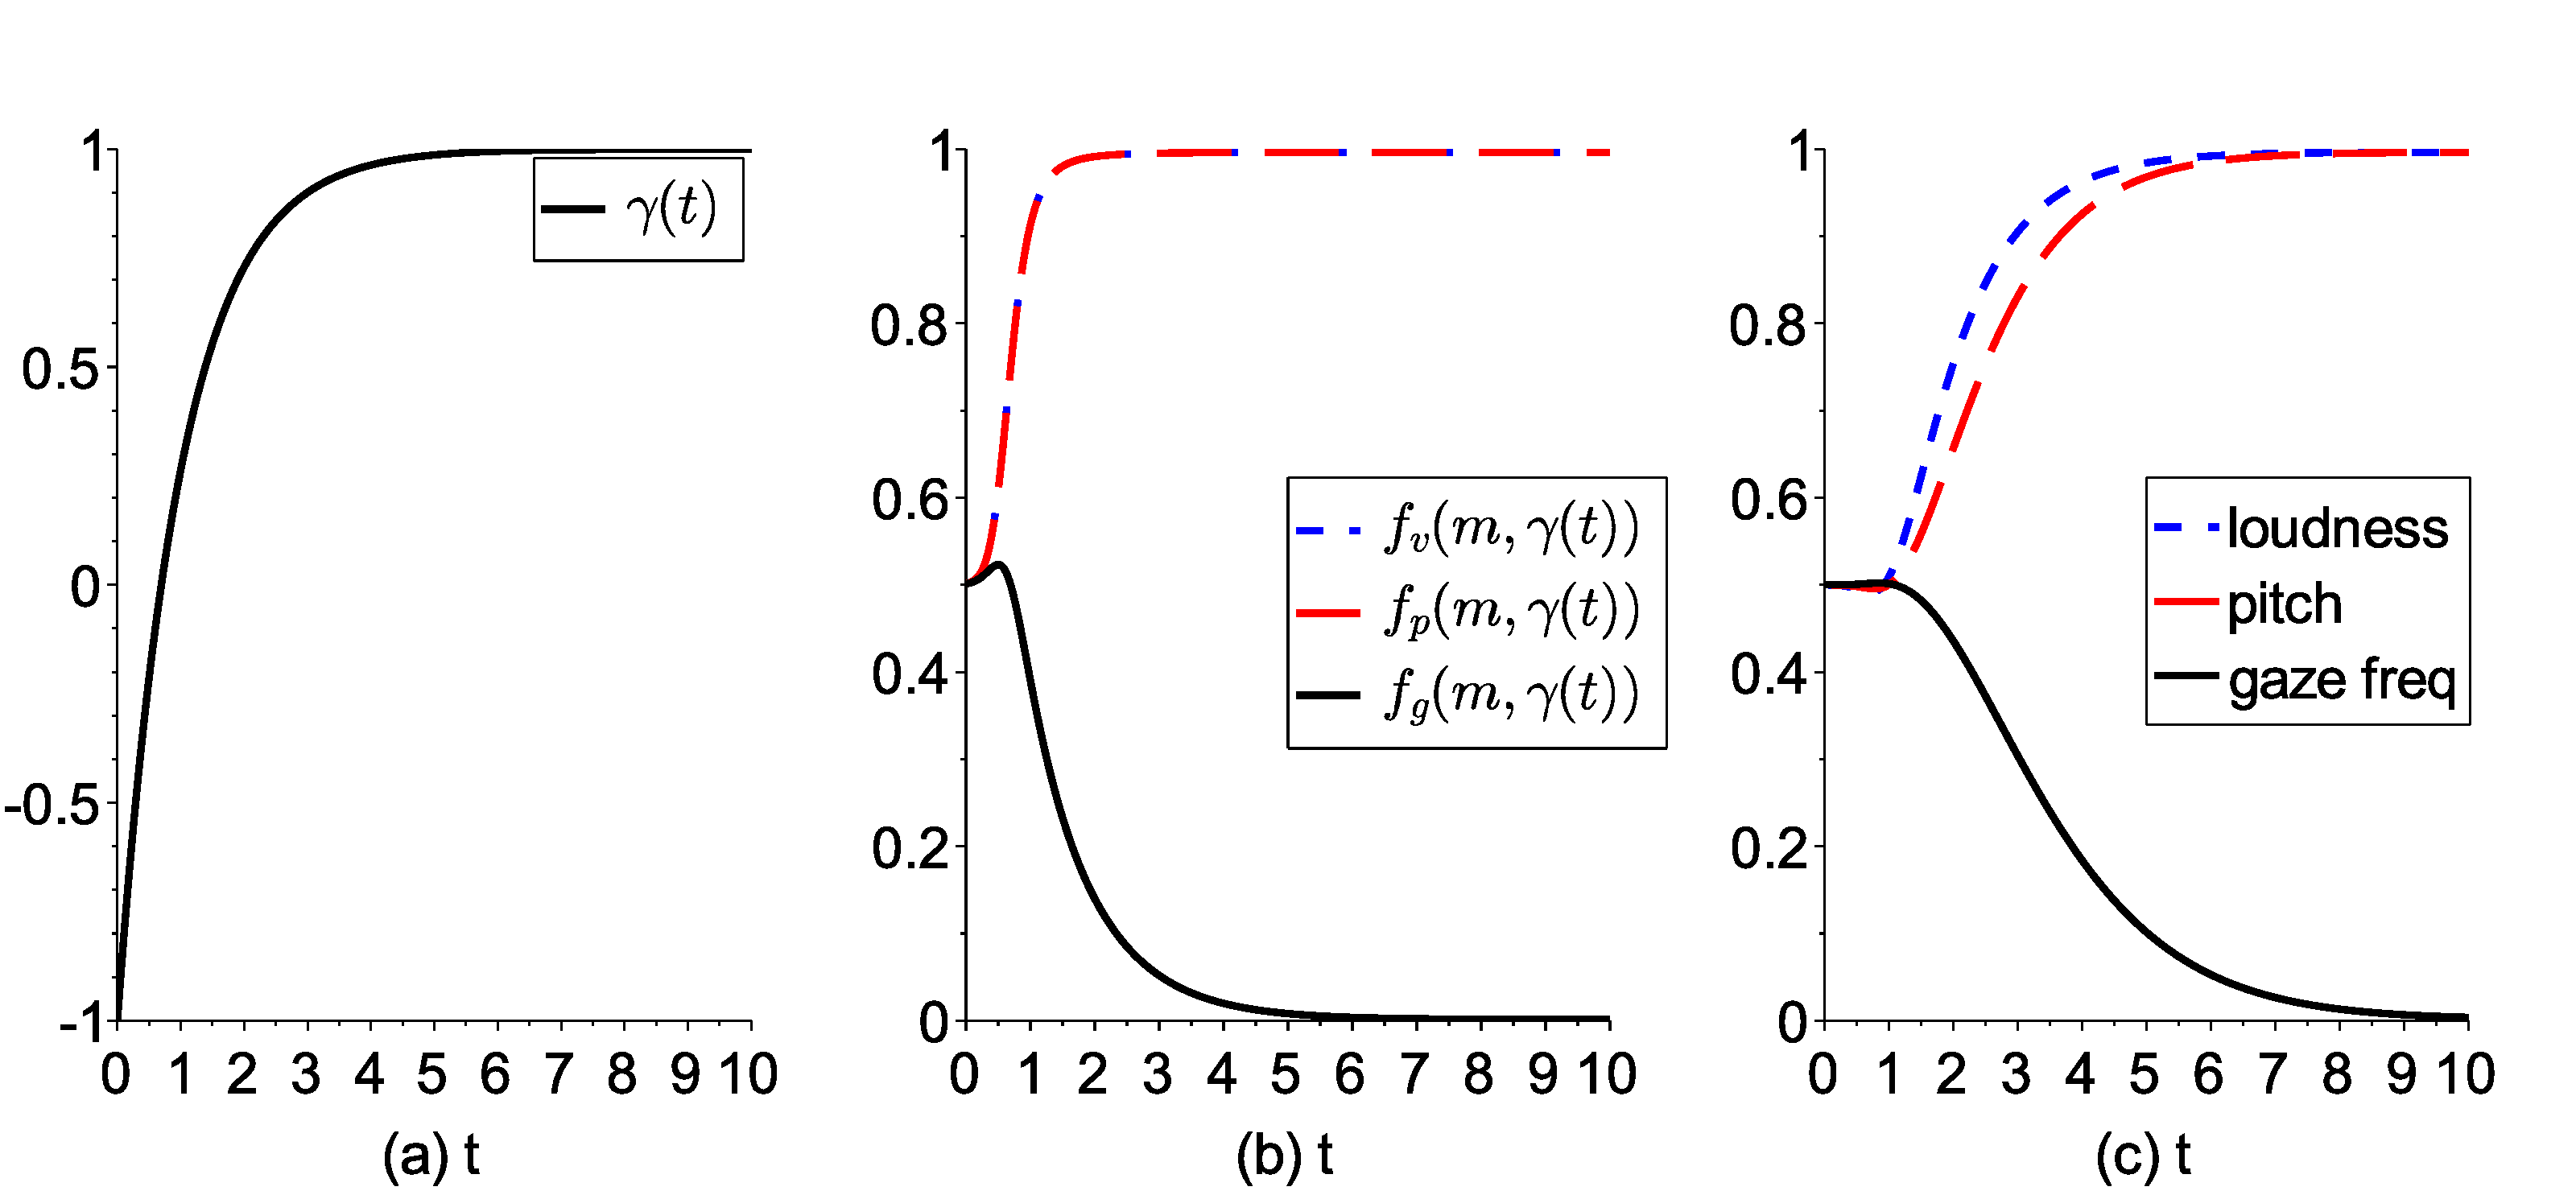
\includegraphics[width=\linewidth]{figure/signals_simu_s2a.pdf}
  \caption{Illustrative simulation S2: time series of the simulated speaker's signal productions. (a) simulation of the agent's perceptual decision-making process (value of $\gamma$). (b) the variations of $f_v(m,\gamma)$, $f_p(m,\gamma)$, $f_r(m,\gamma)$ . (c) resulting  signal productions. Case of an agent with a very strong motivation to keep being the current speaker ($m=-1.0$).}
  \label{demo_simu_l1}
\end{figure}

To illustrate how the agent's motivation impacts the dynamics of the signal production, we simulated the same scenario but with a speaker motivated to yield the turn ($m=1$). As illustrated on Figure \ref{demo_simu}, in this case, $f_v$ and $f_p$ both decreased towards $0$, leading to a variation of the theoretical loudness and pitch towards $0$, illustrating a situation where the agent yielded the turn as it also perceived that the listener was taking the turn. 

\begin{figure}
  \centering
  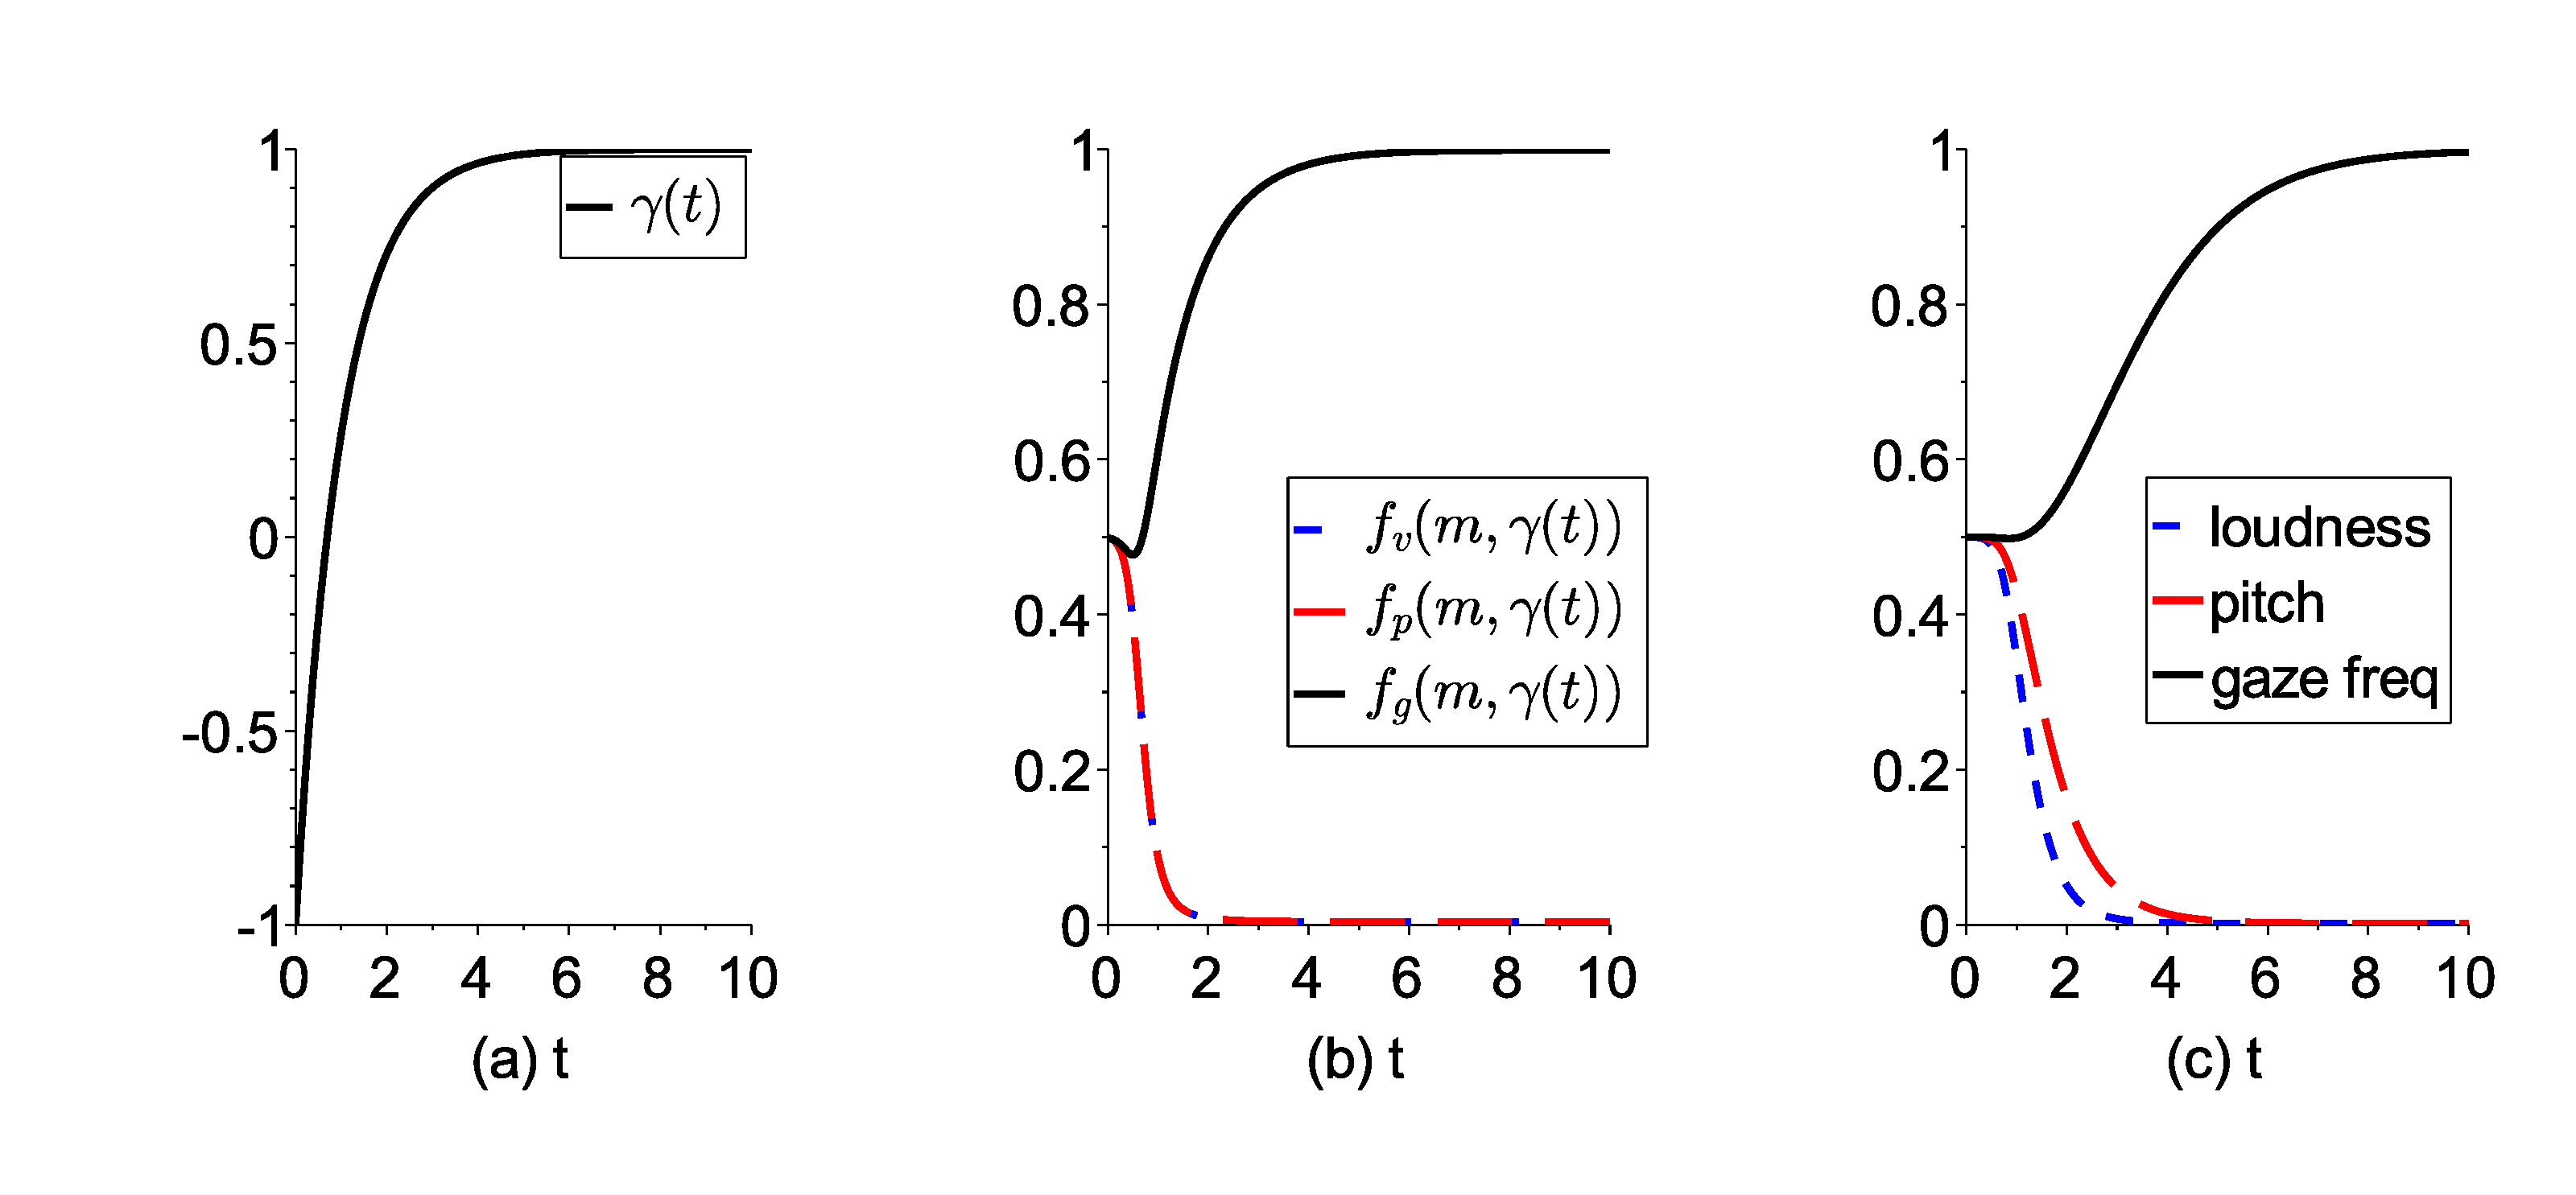
\includegraphics[width=\linewidth]{figure/signals_simu_s2b.pdf}
  \caption{Illustrative simulation S2: time series of the simulated speaker's signal productions. (a) simulation of the agent's perceptual decision-making process (value of $\gamma$). (b) the variations of $f_v(m,\gamma)$, $f_p(m,\gamma)$, $f_r(m,\gamma)$ . (c) resulting  signal productions. Case of an agent with a very strong motivation to leave the turn ($m=1.0$).}
%  \caption{Illustration of a simulation with a simulated variation of the accumulation value. The variation of $f_v(m,\gamma)$, $f_p(m,\gamma)$, $f_r(m,\gamma)$ is illustrated on the middle figure, and the variation of actions on the right figure. In this example the agent has a motivation $m_{sp}=1.0$.}
  \label{demo_simu}
\end{figure}


\section{Properties of the theoretical model}
\label{mod_analysis}

In section \ref{mod_pres}, we have presented separately the two components of our theoretical model. 
We want now to show the relevance of the model for the coordination of speech turns in user-agent interactions.
We demonstrate how the model accounts for the basic features of the interpersonal coordination between participants, namely the capacity to coordinate their turns in various situations, when the agents have compatible goals as well as when they are temporarily in conflicts. In the first case, smooth transitions occur and in the later conflicting overlaps remain limited.
We next show how the model allows the agent to adapt its behavior according to the amount of information it can get about the user's behavior.
All these properties result from the coupling in the signal production of the two interacting participants: the instantaneous behavior of the agent (its signal production) results from the interplay between the variation of its own motivation, with respect to its role in the conversation (speaker versus listener), and its ongoing perceptual decision-making process. 
As a result, the coordination emerges from the interaction between participants, without the support of any explicit algorithm nor set of rules.
This emergence comes from the nature of the equations of the two components of the model (Equations \ref{perc_int}, \ref{alpha_func} and \ref{signal_control}). 

%adaptation to the nature and number of signals exchanged by participants, adaptation to different types of participant and robustness to the noise in the environment. In each case, with the same set of theoretical equations, we will show that participants are still able to coordinate in order to avoid to much unexpected overlap and to have smooth exchange of turns. Such characteristic is fondamental as in real user-agent interactions, the agent rarely interact with the same user and in exactly the same environment. More interesting, we will show that the adaptation and robustness is not due to the nature of the perception equations that would be able to handle several environmnental conditions, but in order to keep an effective coordination, the participants actively modify their signal productions making their behavior clear even in degraded environmnental conditions. 
%We showed the ability of the model to reproduce qualitatively different situations observed during human conversations. 
%for turn-taking management between participants. We presented the overall architecture, and the two different components of our model, namely the behavior perception component and the signal control component. We illustrated how these two component worked separately by simple examples reproducing the dynamics of different situations observed in human conversations. 

%We present thus, in this chapter an analysis of the behavior of two agent interacting according to our theoretical model. 
%We will illustrate the coupled nature of the signal production of the two agents, the overall variations of each agents not controlled only by the agent but also directly influenced by the signal production of the other agent. 
%As a result, the behavior of each agent is emergent of the interaction between participants. 

%We then show that due to the sensorimotor coupling between participants,
 
\subsection{Equations}

As in the previous section, we simulated the interaction between an agent and a hypothetical user. For sake of clarity, lets consider that the agent is the current speaker and the user the current listener, but of course the opposite configuration would give the same results. In this simulated scenario both the agent and the user produced and perceived the same set of signals: volume and pitch of the voice and gaze direction, resp. $v,p,g$.

\subsubsection{Equations of the perceptual decision-making process}

Tables \ref{acc_functions_speaker} and \ref{acc_functions_listener} give the functions that correspond to the different components of Equation \ref{alpha_func}, respectively when the agent is the speaker or the listener. 
The basic assumption, is that each signal perceived by the agent provides some cues about the willingness of its partner to keep or to leave its current role. It is worth noting that these cues may by temporary congruent or in apparent contradiction.
We set these partial accumulation functions such as the agent interpret similar signals variations as we observed in human conversations. For a listener agent, values of loudness and pitch less than $0.4$ and the partner looking towards the agent (gaze value more than 0.5) are end of turns cues, whereas loudness and pitch values higher than $0.5$, and a speaker averting its gaze (gaze value less than 0.5) from the agent are more turn keeping values. For a speaker agent, values of loudness and pitch indicating that the user is starting to speak (in our example higher than $0.1$) and averting his gaze (gaze value less than 0.5) from the agent are turn taking cues.

%We defined then the function determining the attractor values for the agents. These functions represents the $f(m(t),\gamma(t))$ part of the signal control equation \ref{signal_control}. The equation \ref{loc_vol_pit} represents the loudness and pitch control equation, and the equation \ref{loc_gaze} represents the gaze control equation. 

\begin{table}
\centering
\begin{tabular}{|c|c|c|}
\hline
Cue & Speaker \\
\hline
Loudness & $\alpha_{v_{loc}}(v,\dot{v})=1.5\times (v-0.1)$ \\
\hline
Pitch & $\alpha_{p_{loc}}(p,\dot{p})=1.5\times (p-0.1)$ \\
\hline
Gaze & $\alpha_{g_{loc}}(g,\dot{g})=-1.5\times (g-0.5)$ \\
\hline
\end{tabular}
\caption{Set of accumulation functions used in Equation \ref{alpha_func} for the speaker.}
\label{acc_functions_speaker}
\end{table}

\begin{table}
\centering
\begin{tabular}{|c|c|c|}
\hline
Cue & Listener \\
\hline
Loudness & $\alpha_{v_{lis}}(v,\dot{v})=-2.0\times (v-0.4)$ \\
\hline
Pitch & $\alpha_{p_{lis}}(p,\dot{p})=-2.0\times (p-0.4)$ \\
\hline
Gaze & $\alpha_{g_{lis}}(g,\dot{g})=1.0\times (g-0.5)$ \\
\hline
\end{tabular}
\caption{Set of accumulation functions used in Equation \ref{alpha_func} for the listener.}
\label{acc_functions_listener}
\end{table}

\subsubsection{Equations of signal production}

For the simulation of the speaker's behavior, we used the set of equations \ref{eq_speaker_pitch}, \ref{eq_speaker_volume}, \ref{eq_speaker_gaze} and \ref{eq_sigmoid}. Figures \ref{fig_pro_loc} and \ref{fig_gaze_loc} represent the resulting values of $v_{loc}$, $p_{loc}$ and $g_{loc}$, computed using Equation \ref{signal_control}.

\begin{figure}
\centering
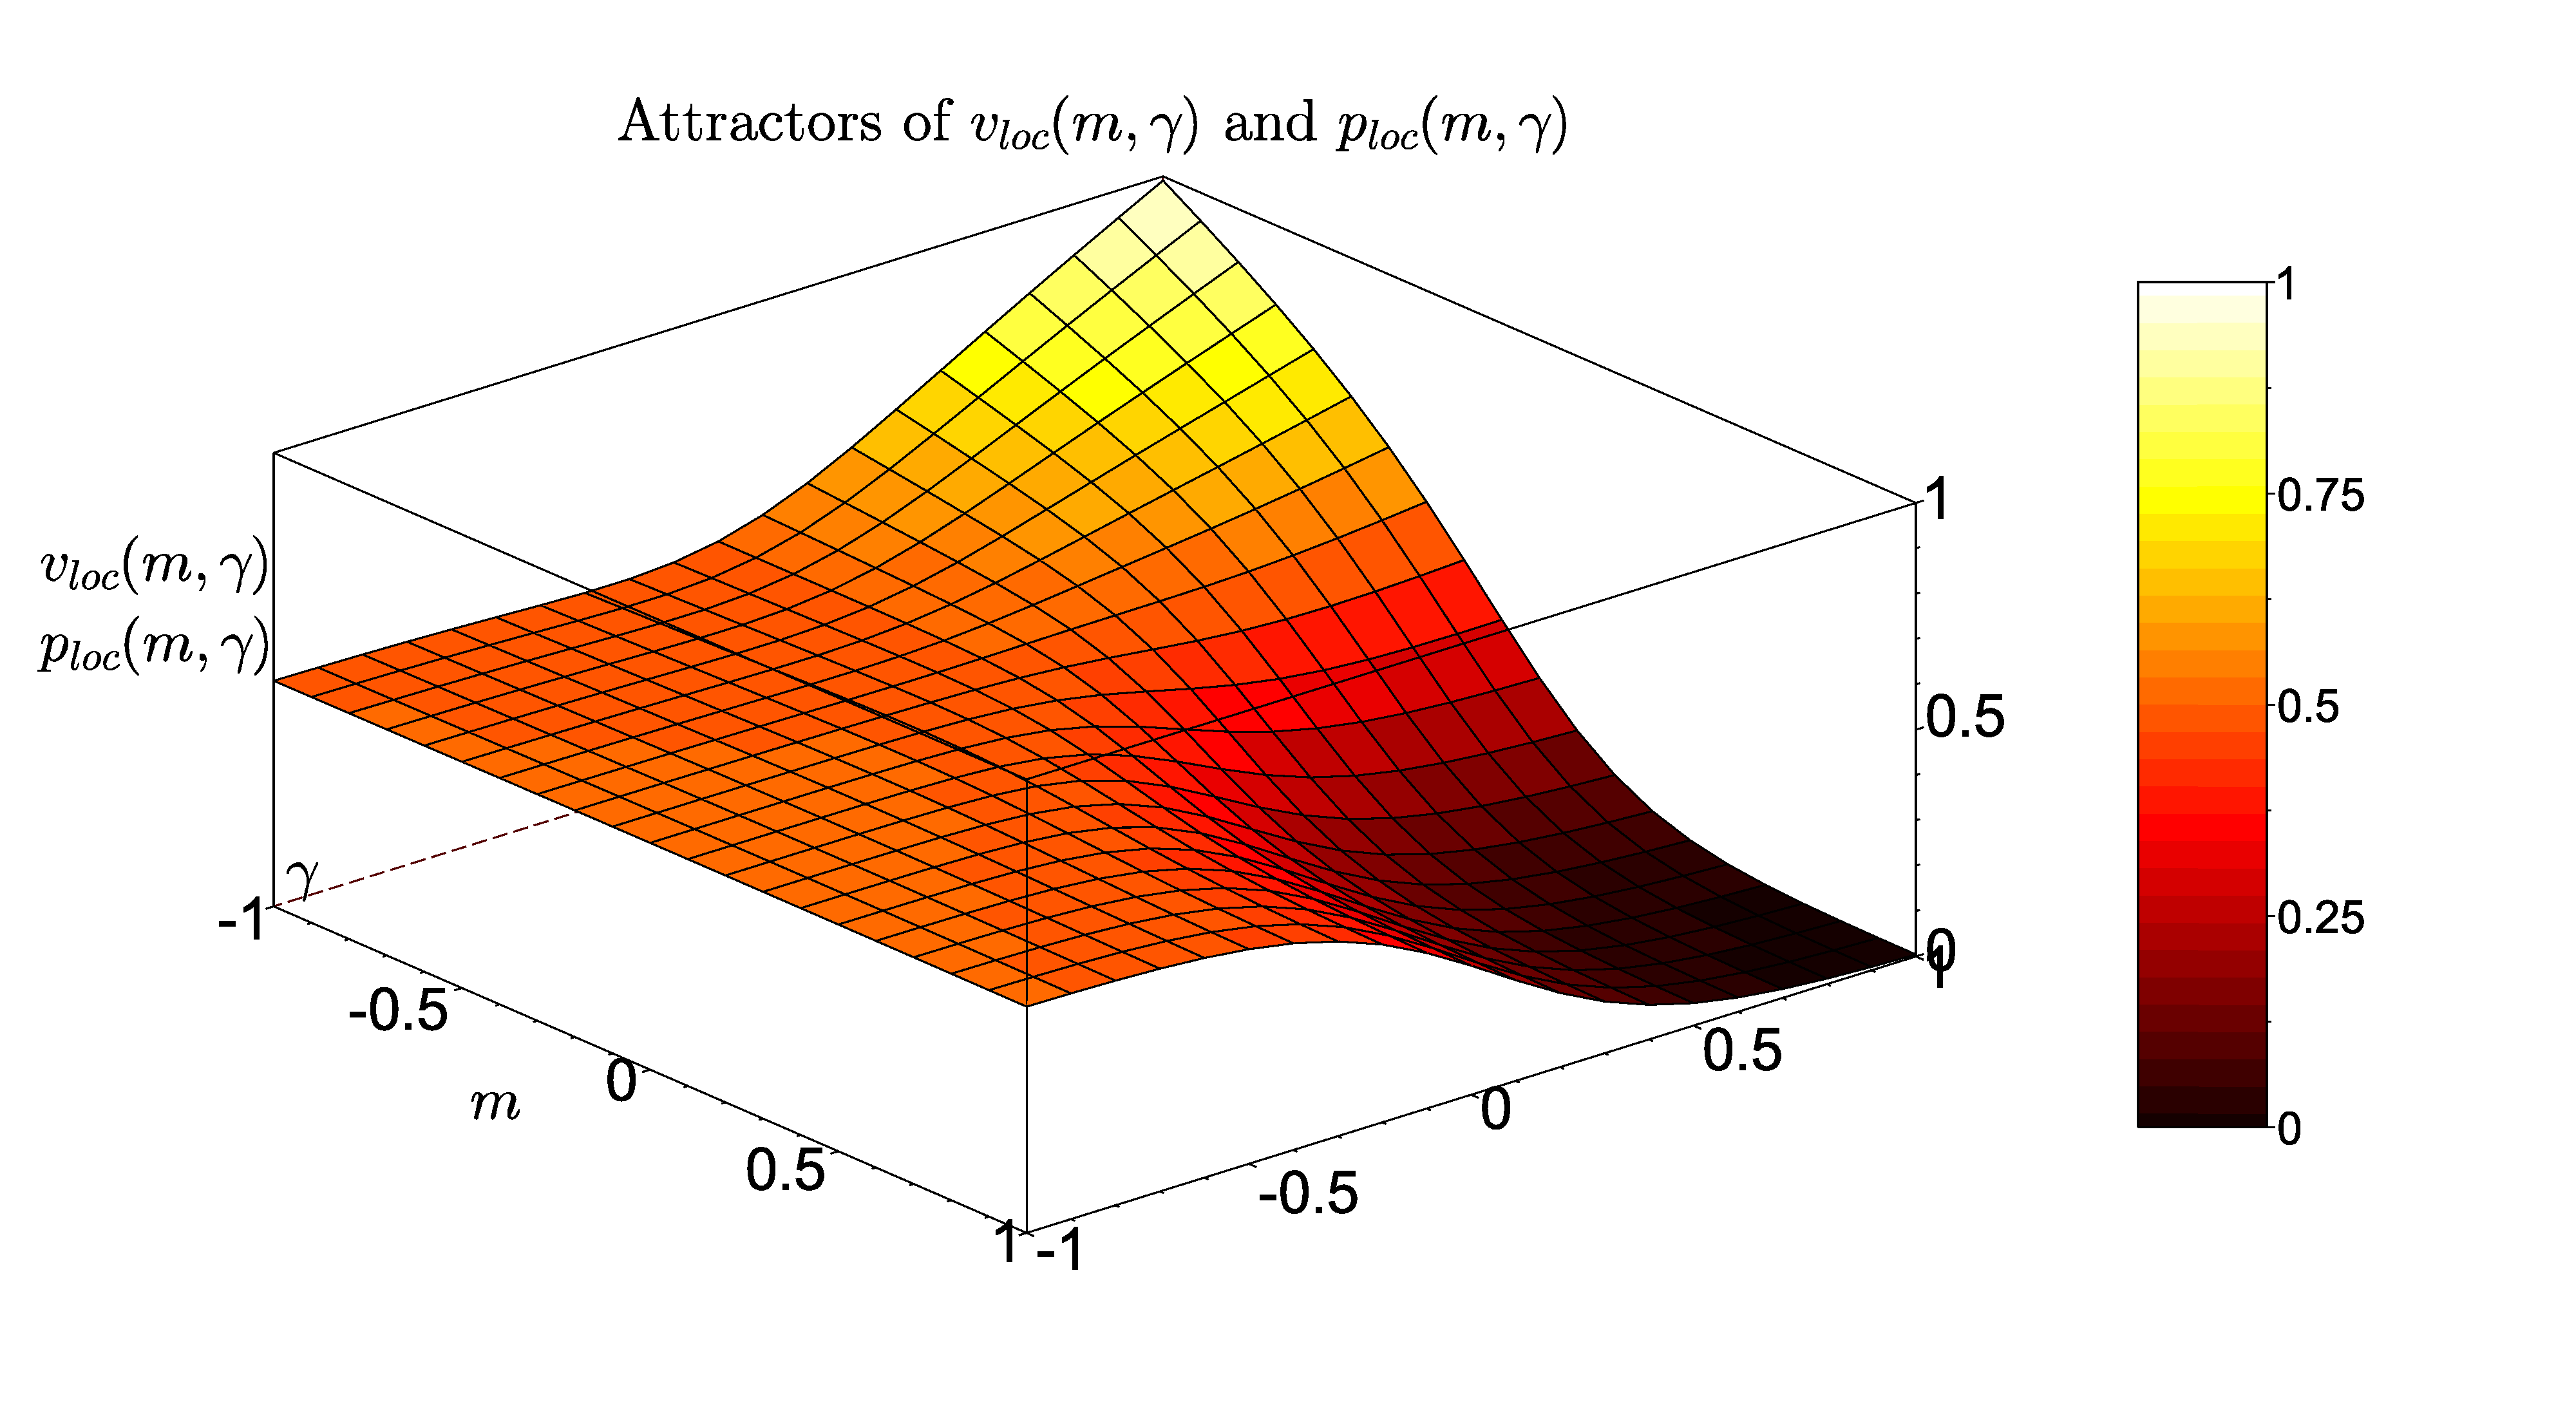
\includegraphics[width=\linewidth]{figure/bifurcProsodyLoc.pdf}
\caption{Values of $v_{loc}$ and $p_{loc}$ as functions of $m(t)$ and $\gamma(t)$.}
\label{fig_pro_loc}
\end{figure}

\begin{figure}
\centering
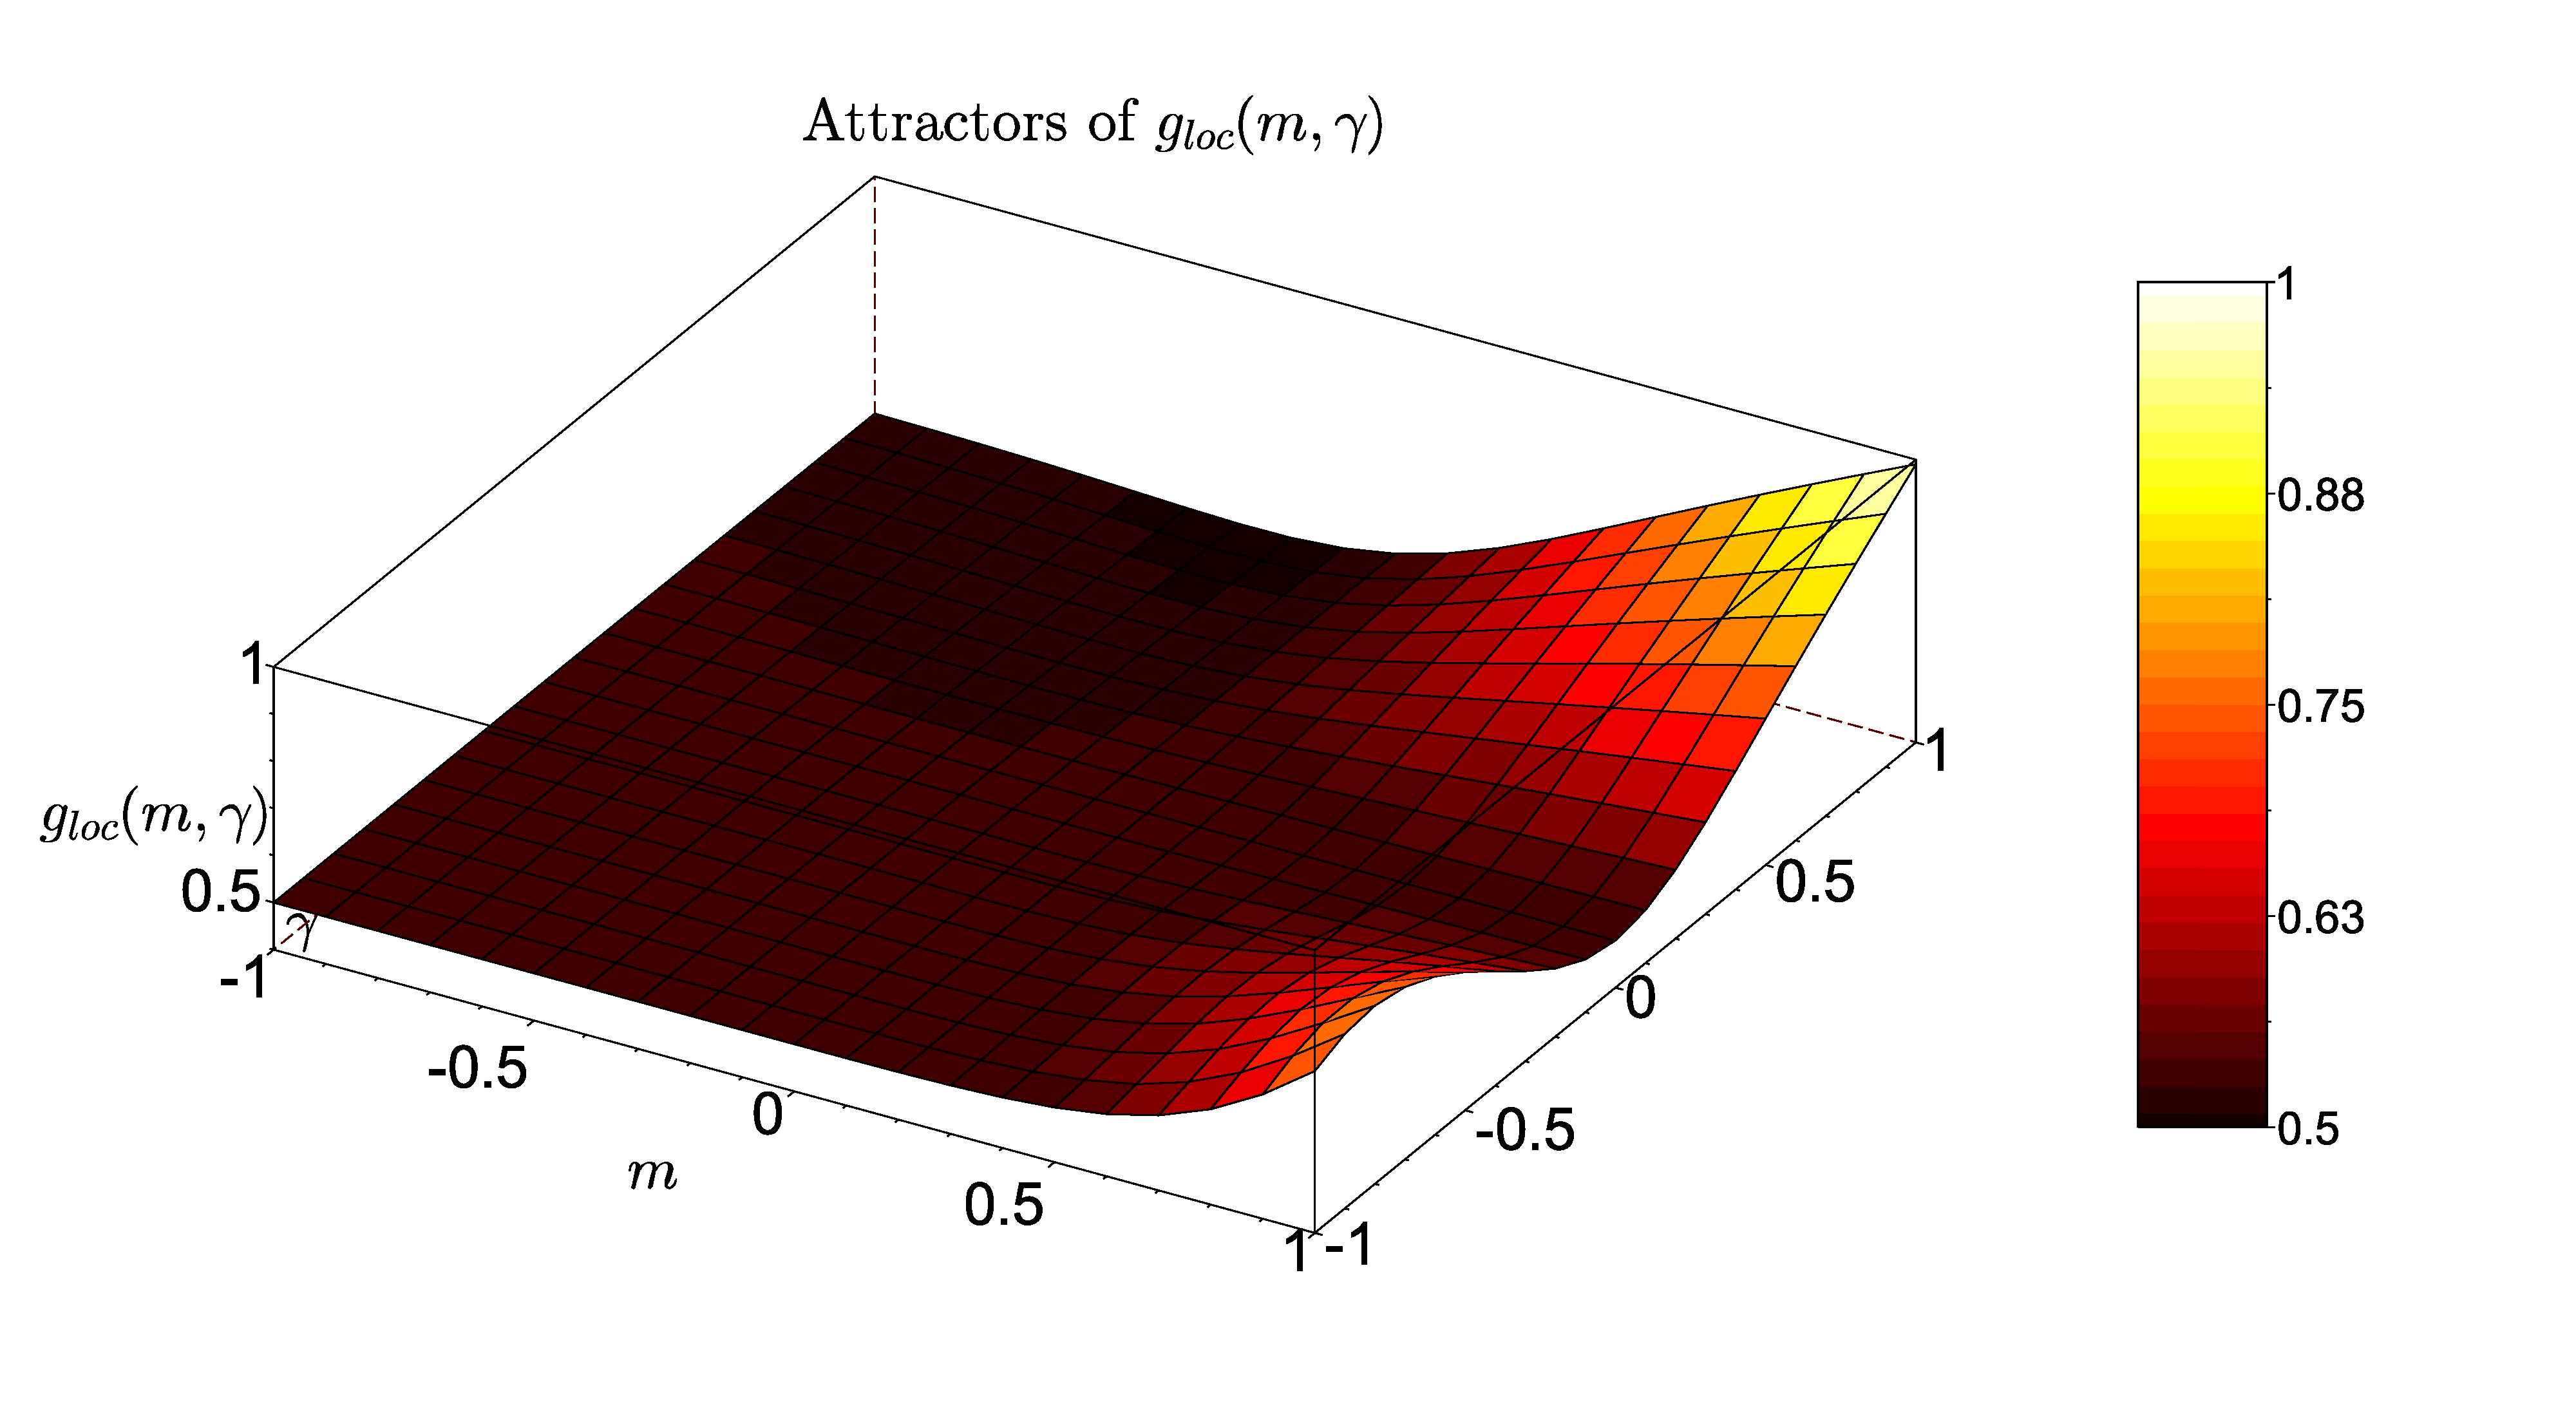
\includegraphics[width=\linewidth]{figure/gazeLoc.pdf}
\caption{Values of $g_{loc}(m,\gamma)$}
\label{fig_gaze_loc}
\end{figure}

%Before showing our simulations, we present here the equations used in the following to illustrate the properties of our model. The agents modulate three types of signals, loudness, pitch and gaze. The values of these signals have the same meaning as presented in section \ref{mod_pres}. A loudness value equal to $0$ indicates an agent that stopped speaking, a loudness value equal to $1$ the loudest value with which the participant can talk, and $0.5$ the agent's loudness mean value. Pitch follows the same logic except that a $0$ value means the minimal non nul value of pitch. For gaze, $1$ indicate an agent look permantently at the user, $0$ means the agent never look to the user, $0.5$ that the agent varies its gaze in order that 50 \% of time it looks at its partner and 50 \% it looks elsewhere. We define for each value the accumulation functions presented in the tables \ref{acc_functions_sp} and \ref{acc_functions_list}. 

% \begin{equation}
% \begin{array}{l l l}
% v_{loc}&=p_{loc}&=0.5 \\
% &&-0.5\times \gamma \times m \times S(-m)\times S(\gamma) \\
% &&-0.5\times S(\gamma) \times S(m)\\
% S(x)&&=\frac{1}{1+\exp(-10.0\times x)}
% \end{array}
% \label{loc_vol_pit}
% \end{equation}

% \begin{equation}
% \begin{array}{l l}
% g_{loc}&=0.5 \\
% &+0.5\times \gamma \times m \times S(\gamma) \times S(m) \\
% &-0.5 \times \gamma \times m \times S(\gamma(t) + m(t)) \times S(-\gamma) \times S(m) \\
% S(x)&=\frac{1}{1+\exp(-10.0\times x)}
% \end{array}
% \label{loc_gaze}
% \end{equation}

% $v_{loc}$, $p_{loc}$ and $g_{loc}$ corresponds respectively to the loudness, pitch and gaze variations. In each equations, $S(x)$ corresponds to the same sigmoid functions as used in the equation \ref{attr_foncs}, and serve the same goal as for the equations \ref{attr_foncs}. For example, the term $-0.5 \times \gamma \times m \times S(\gamma(t) + m(t)) \times S(-\gamma) \times S(m)$ is greater than $0$ if $\gamma(t)<0$, $m(t)>0$ and $\gamma(t)<-m(t)$. 

% The equations \ref{loc_vol_pit} and \ref{loc_gaze} has been defined such as the value of loudness and pitch when the partner doesn't display any turn-taking cues, that is, when the accumulation value is less than $0$ corresponds to the mean value $0.5$. 
% When $m(t)<0$ and $\gamma(t)>0$, the agent wants to keep its role and perceive that its partner is taking turn, it then increases its loudness and pitch and averts its gaze as observed in human conversations \citep{kurtic_resources_2013}. When $m(t)>0$ and $\gamma(t)>0$, the agent wants to yield its turn and perceives that its partner is taking turn, he then decreases its volume and pitch values and look towards its partner similar to what happens in human conversations \citep{gravano_turn-taking_2011,novick_coordinating_1996}. 

For the listener, the functions governing the variation of the attractor of Equation \ref{signal_control} are as follows:
 
\begin{equation}
f_{v_{lis}}= f_{p_{lis}} = \frac{1}{2} \gamma S(m+\gamma) + S(m+\gamma)S(m)S(-\gamma)
\label{lis_pro}
\end{equation}

\begin{equation}
f_{g_{lis}} = 1 - S(m + \gamma)
\label{lis_gaze}
\end{equation}

These equations has been defined such as, when the speaker produces no cues, the values of loudness and pitch equal $0$, and the gaze value equals $1$: the listener is silent and is constantly fixing its gaze toward the speaker. 
According to these equations, when $m(t)<0$ and $\gamma(t)>0$ and $|\gamma(t)|>|m(t)|$, or when $m(t)>0$ and $\gamma(t)<0$ and $|\gamma(t)|>|m(t)|$, the listener will try to grab or take the turn by increasing its loudness and pitch values and averting its gaze from the current speaker. Figures \ref{fig_pro_lis} and \ref{fig_gaze_lis} illustrate the distribution of the attractors of Equation \ref{signal_control}, using Equations \ref{lis_pro} and \ref{lis_gaze}.

%The formulation of these equations permit to make the agent signal control equations depending on the relationship between the motivation of the agent and the strength of the cues displayed by the agent's partner. 
Figures \ref{fig_pro_loc} to \ref{fig_gaze_lis} illustrate the dynamic interplay between the agent's intrinsic motivation and the influence of the agent's partner behavior.
During the interaction $m$ and $\gamma$ are continuously varying, which results in the continuous modulation of the agent's prosodic and non verbal signals production. Because the $\gamma$ of each agent depends on the signals $s_j$ produced by the other agent, the model accounts for the coupling of the two agents. This coupling make the agent's nonverbal signals following an emergent trajectory. The next section illustrates how the turn-taking behavior, and more generally the coordination, emerges from this complex dynamics. 

% COMMENT Pierre : ce qui est explique en dessous est 2 situations compliquees - pas facile a comprendre. Il vaut miuex le voir dans la section suivante.
%For instance, the higher the listener's motivation to change role the more it will need a strong accumulation value to begin to display turn-yielding cues. In this sense, the agent will more or less resist to the perception of the speaker keeping the turn, resulting in a conflict lasting more or less. On the opposite, when the agent has a motivation to stay listener, the higher the motivation of the agent, the more the agent will ``resist" to the perception of its partner yielding its turn by staying listener. In this case, if the accumulation value is sufficiently high compared to the motivation of the agent, the agent will take the turn, as if it was forced to take it. 

\begin{figure}
  \centering
  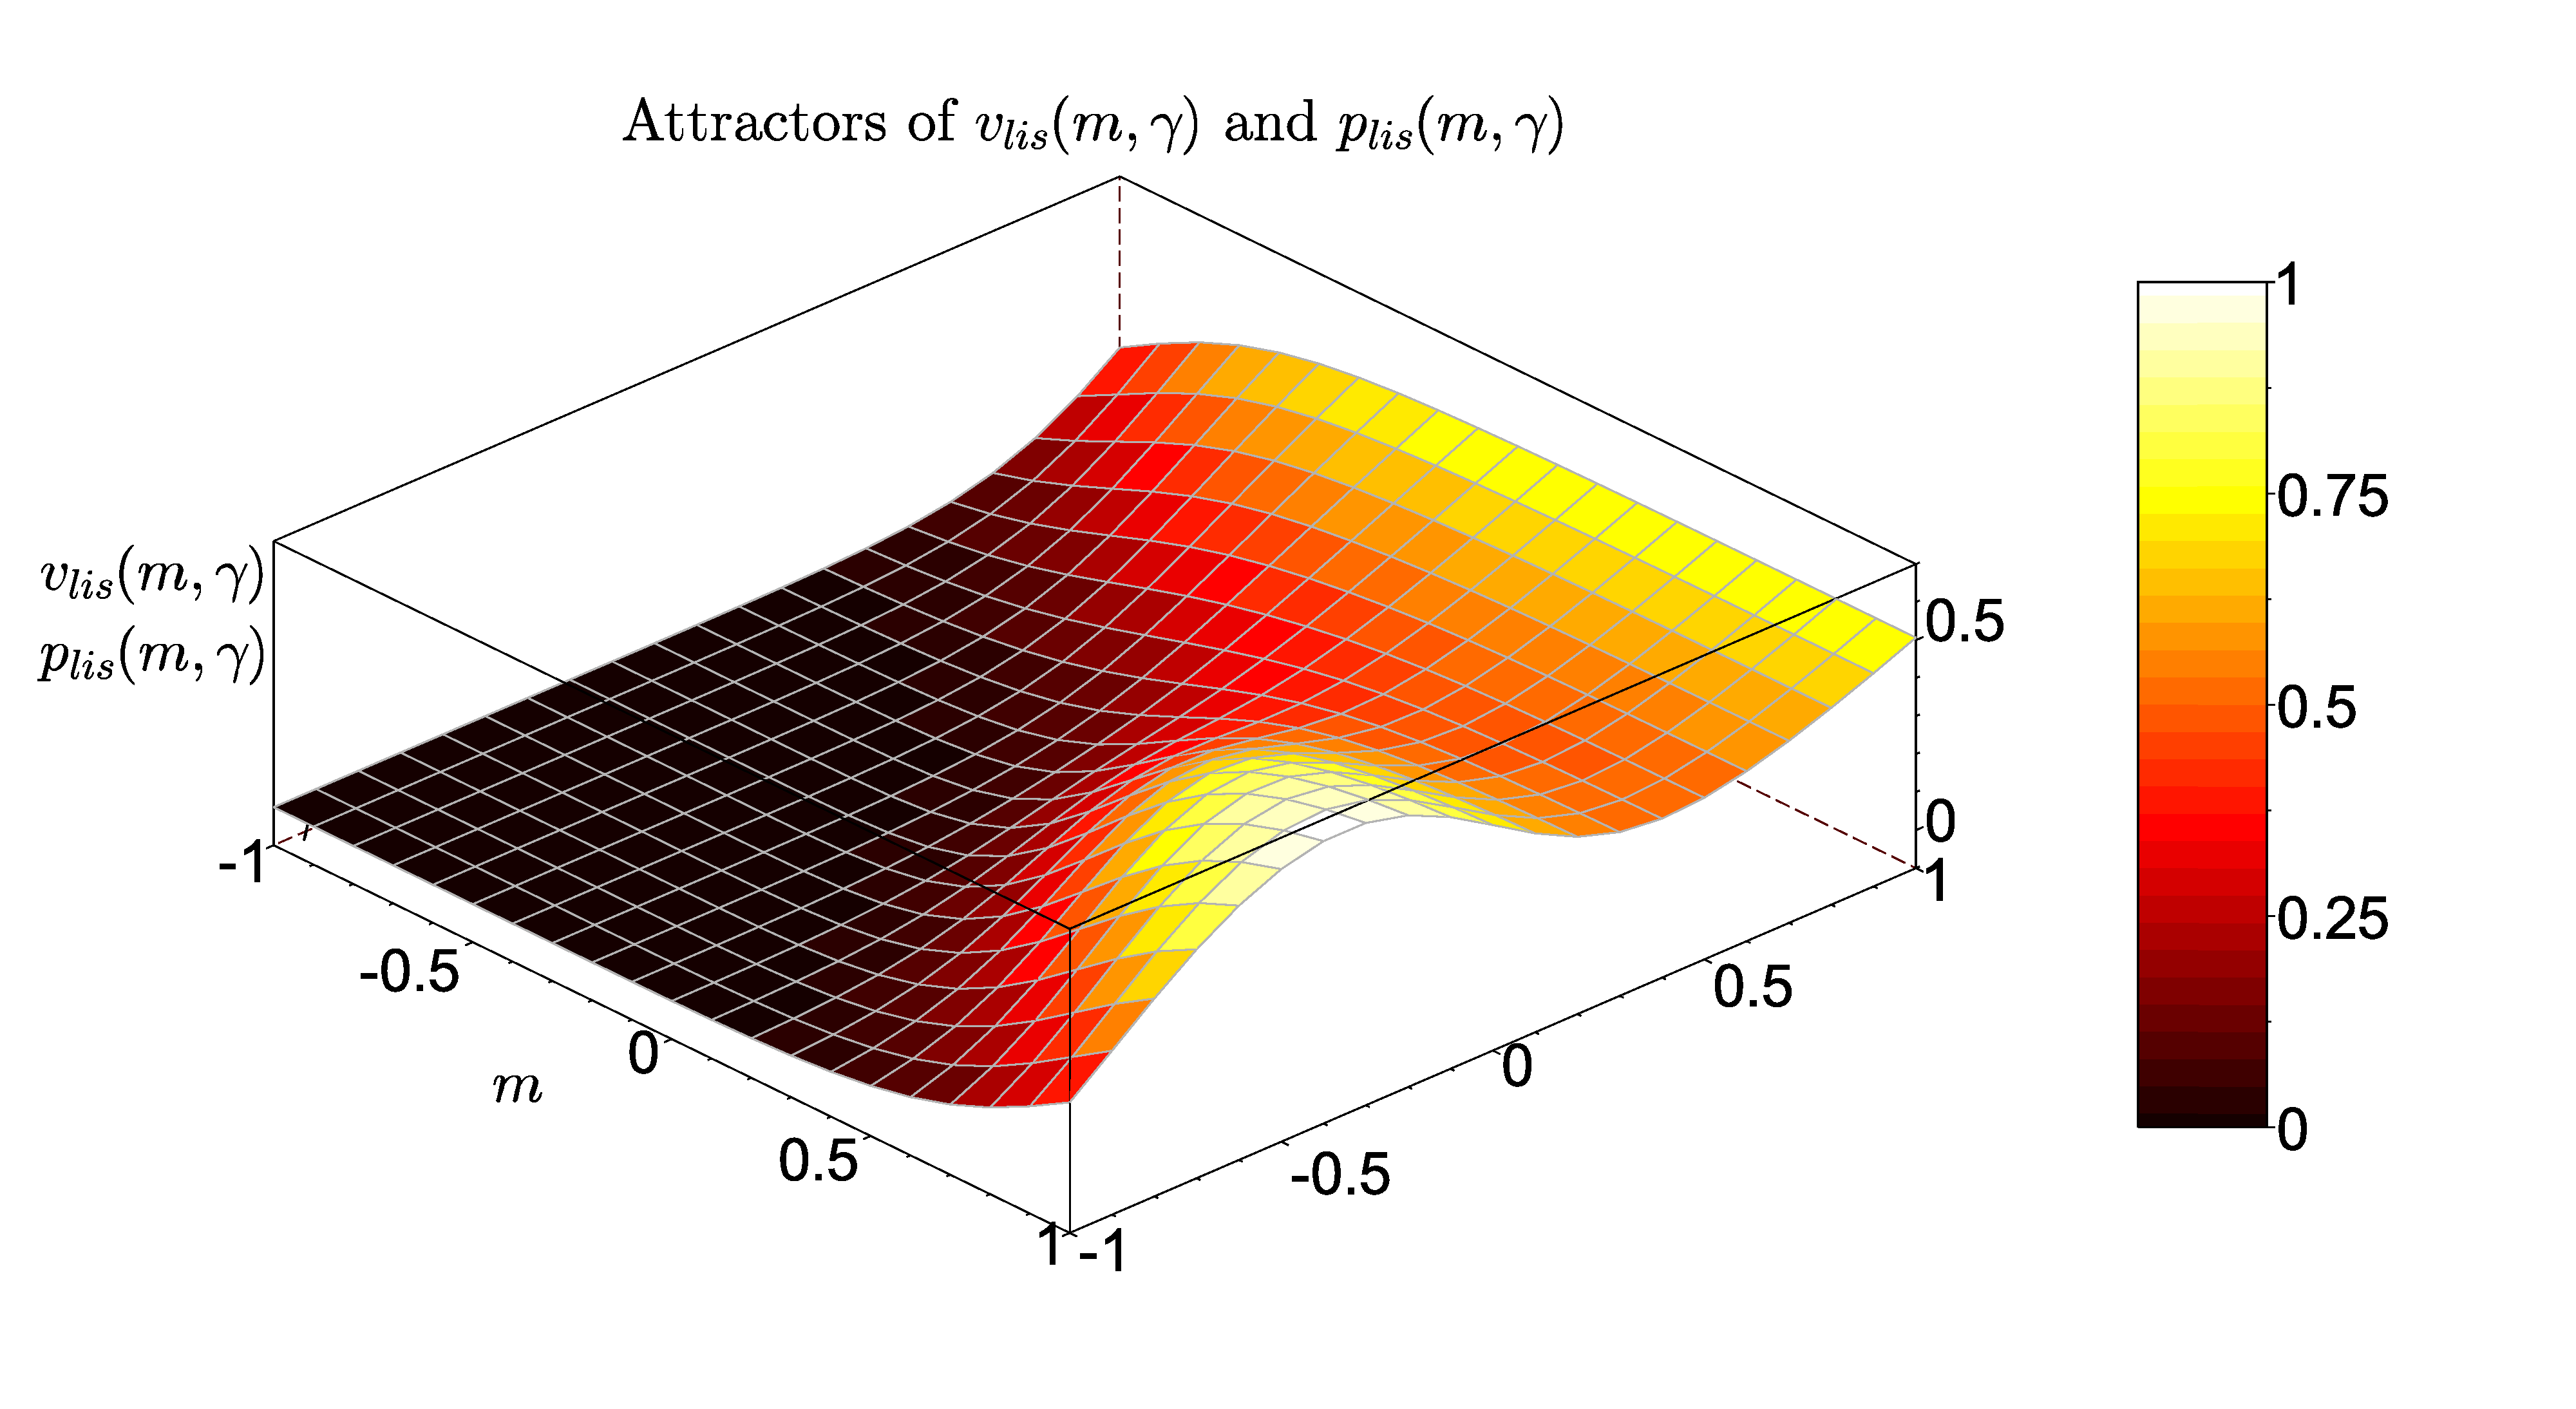
\includegraphics[width=\linewidth]{figure/bifurcProsodyLis.pdf}
  \caption{Values of $v_{lis}(m(t),\gamma(t))$ and $p_{lis}(m(t),\gamma(t))$}
  \label{fig_pro_lis}
\end{figure}

\begin{figure}
  \centering
  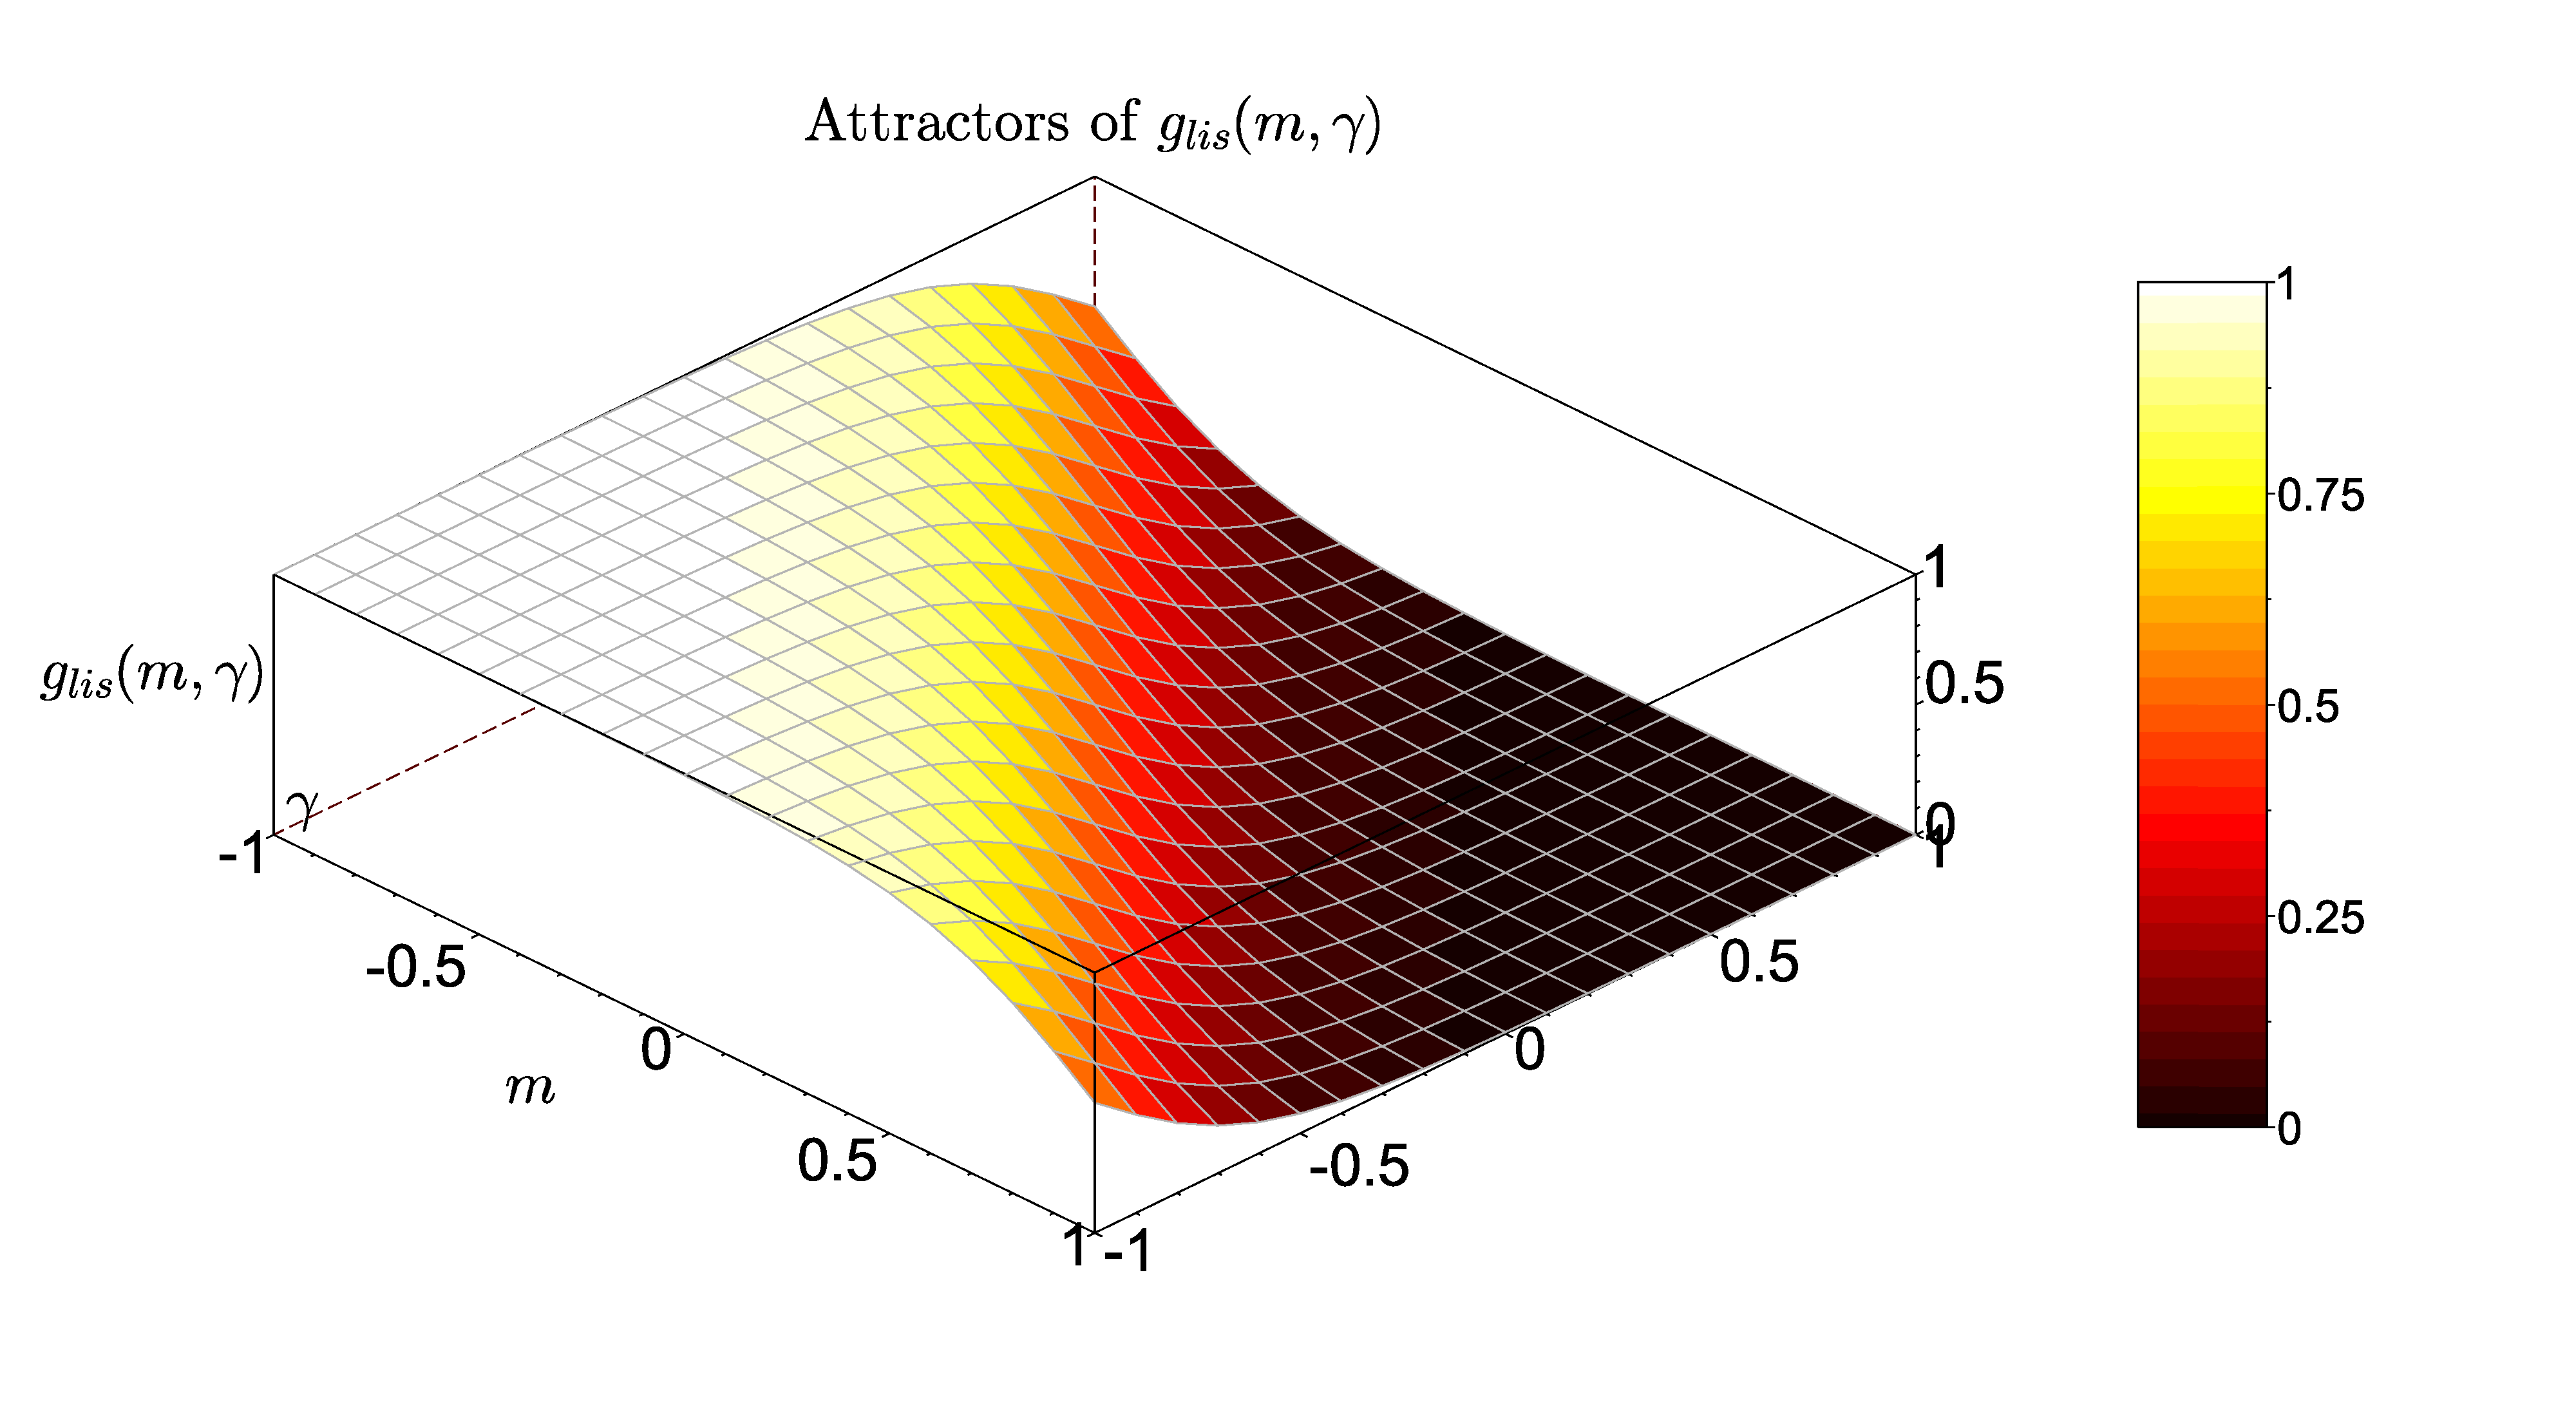
\includegraphics[width=\linewidth]{figure/gazeLis.pdf}
  \caption{Values of $g_{lis}(m(t),\gamma(t))$}
  \label{fig_gaze_lis}
\end{figure}

\subsection{Emergence of behavior}

%Based on the different theoretical equations, our aim in this section is now to show the capability of our model to make emerge the different situations linked to turn-taking. What is important about our model is the fact that the signal variations of the participants are determined not only by the motivations, that is the initial goals the participants have towards the coordination of speaking turns, either changing or keeping its role, but also directly by the accumulation value directly varying according the different signal variations of the agent's partner. As a result, we can't predict the final behavior of the agent, that is, the temporal evolution of the signal productions, but this behavior is an emergent property of the interaction between the participants. 

In the previous section, we analysed the dynamics of the state variable $\gamma$ as a response of the agent's intrinsic motivation $m$, which acts as a forcing variable of our model. In this section, we explain how the two agents coordinate their speech turns in various situations, although they are not endowed with any explicit coordination algorithm. We show that the model accounts for the different situations observed in human conversation and that the moment of time when the transition of turns occurs, or how long competitive overlaps last is not under the control any specific agent, but dynamically emerges from the interaction. Indeed, we illustrate this emergence on three contrasting scenarios, summarized in Table \ref{tab_scenarios_emergence}, that show that varying the motivation of only one of the two participants strongly change the behavior of the other participant. For sake of demonstration, in these simulations, the agents' motivation remained constant during the whole interaction. 

% COMMENT: on commence par le plus simple pour que le lecteur comprenne bien.
\begin{table}
  \begin{center}
    \begin{tabular}{ccc}
      \hline
      \mbox{} & Speaker's goal, $G_{loc}$ & Listener's goal $G_{lis}$\\
      \hline
      S3 & opposite, $m=1.0$ & strong, $m=1.0$\\
      \hline
      S4 & strong, $m=-1.0$ & strong, $m=1.0$\\
      \hline
      S5 & strong, $m=-1.0$ & low, $m=0.15$\\
      \hline
    \end{tabular}
  \end{center}
  $G_{loc}$: go on speaking (keep the same goal)\linebreak
  $G_{lis}$: say something (change to the opposite role)

  \caption{Scenarios for the analysis of the emerging behavior. Values of the forcing variable $m$ for the two agents.}
  \label{tab_scenarios_emergence}
\end{table}

\begin{figure}[b]
  \centering
  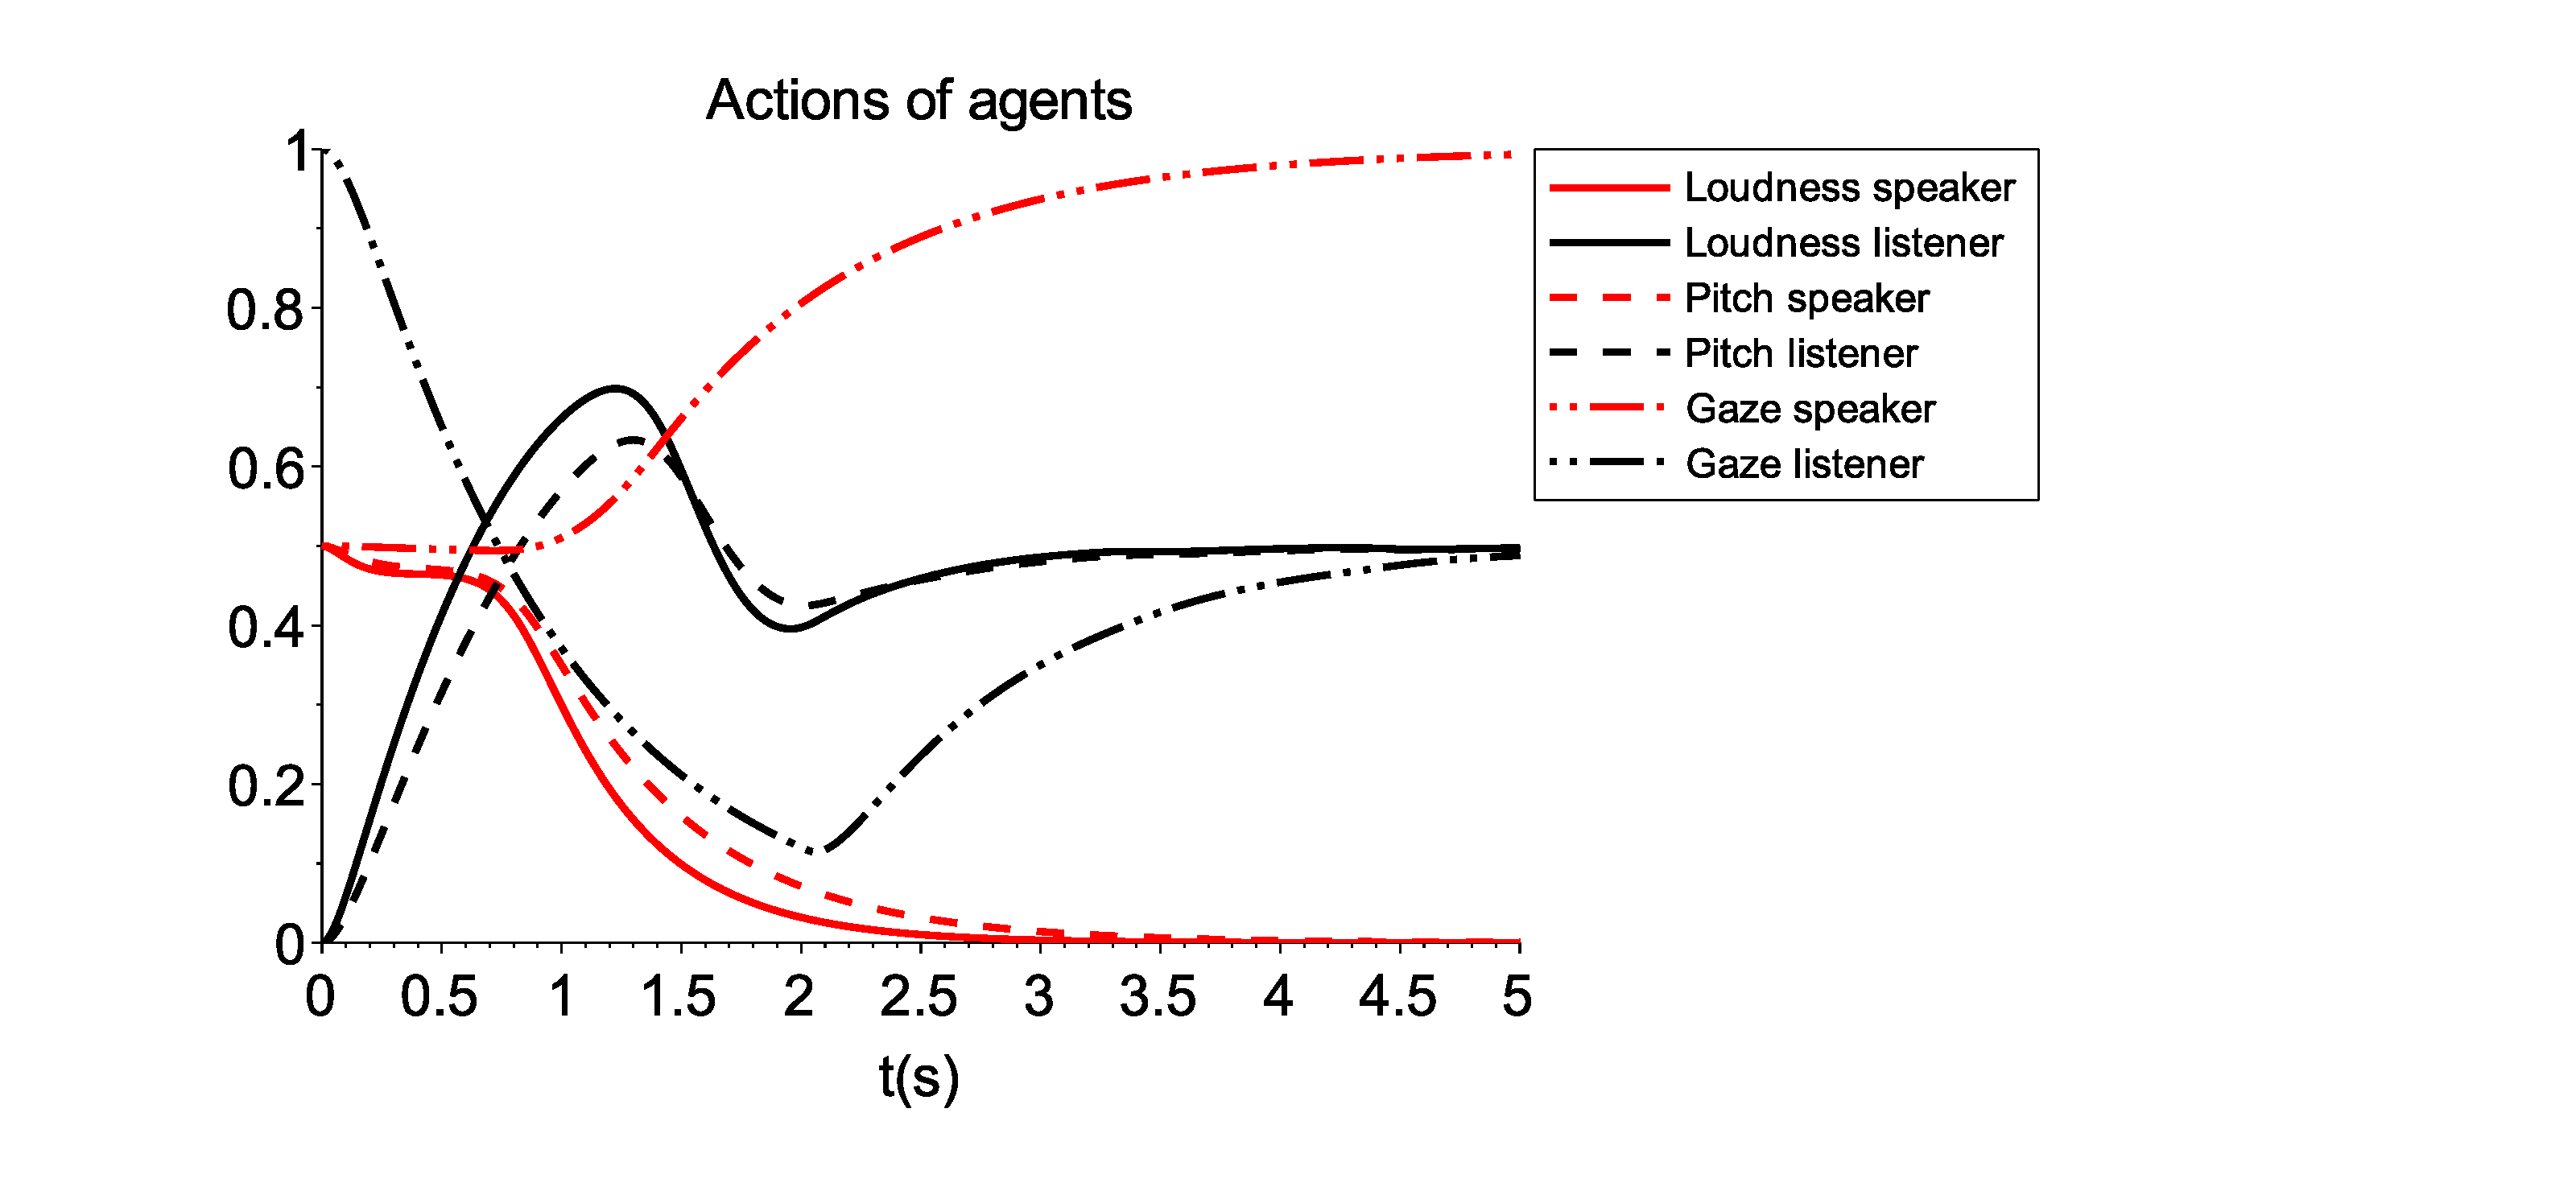
\includegraphics[width=\linewidth]{figure/smooth-transition_signal-production.pdf}
  \caption{Modulation of the verbal and non verbal signals produced by the two agents. The resulting behavior is a smooth transition of the turn from the current speaker to the current listener. Scenario S3} 
  \label{simu_smooth}
\end{figure}

\begin{figure}[t]
  \centering
  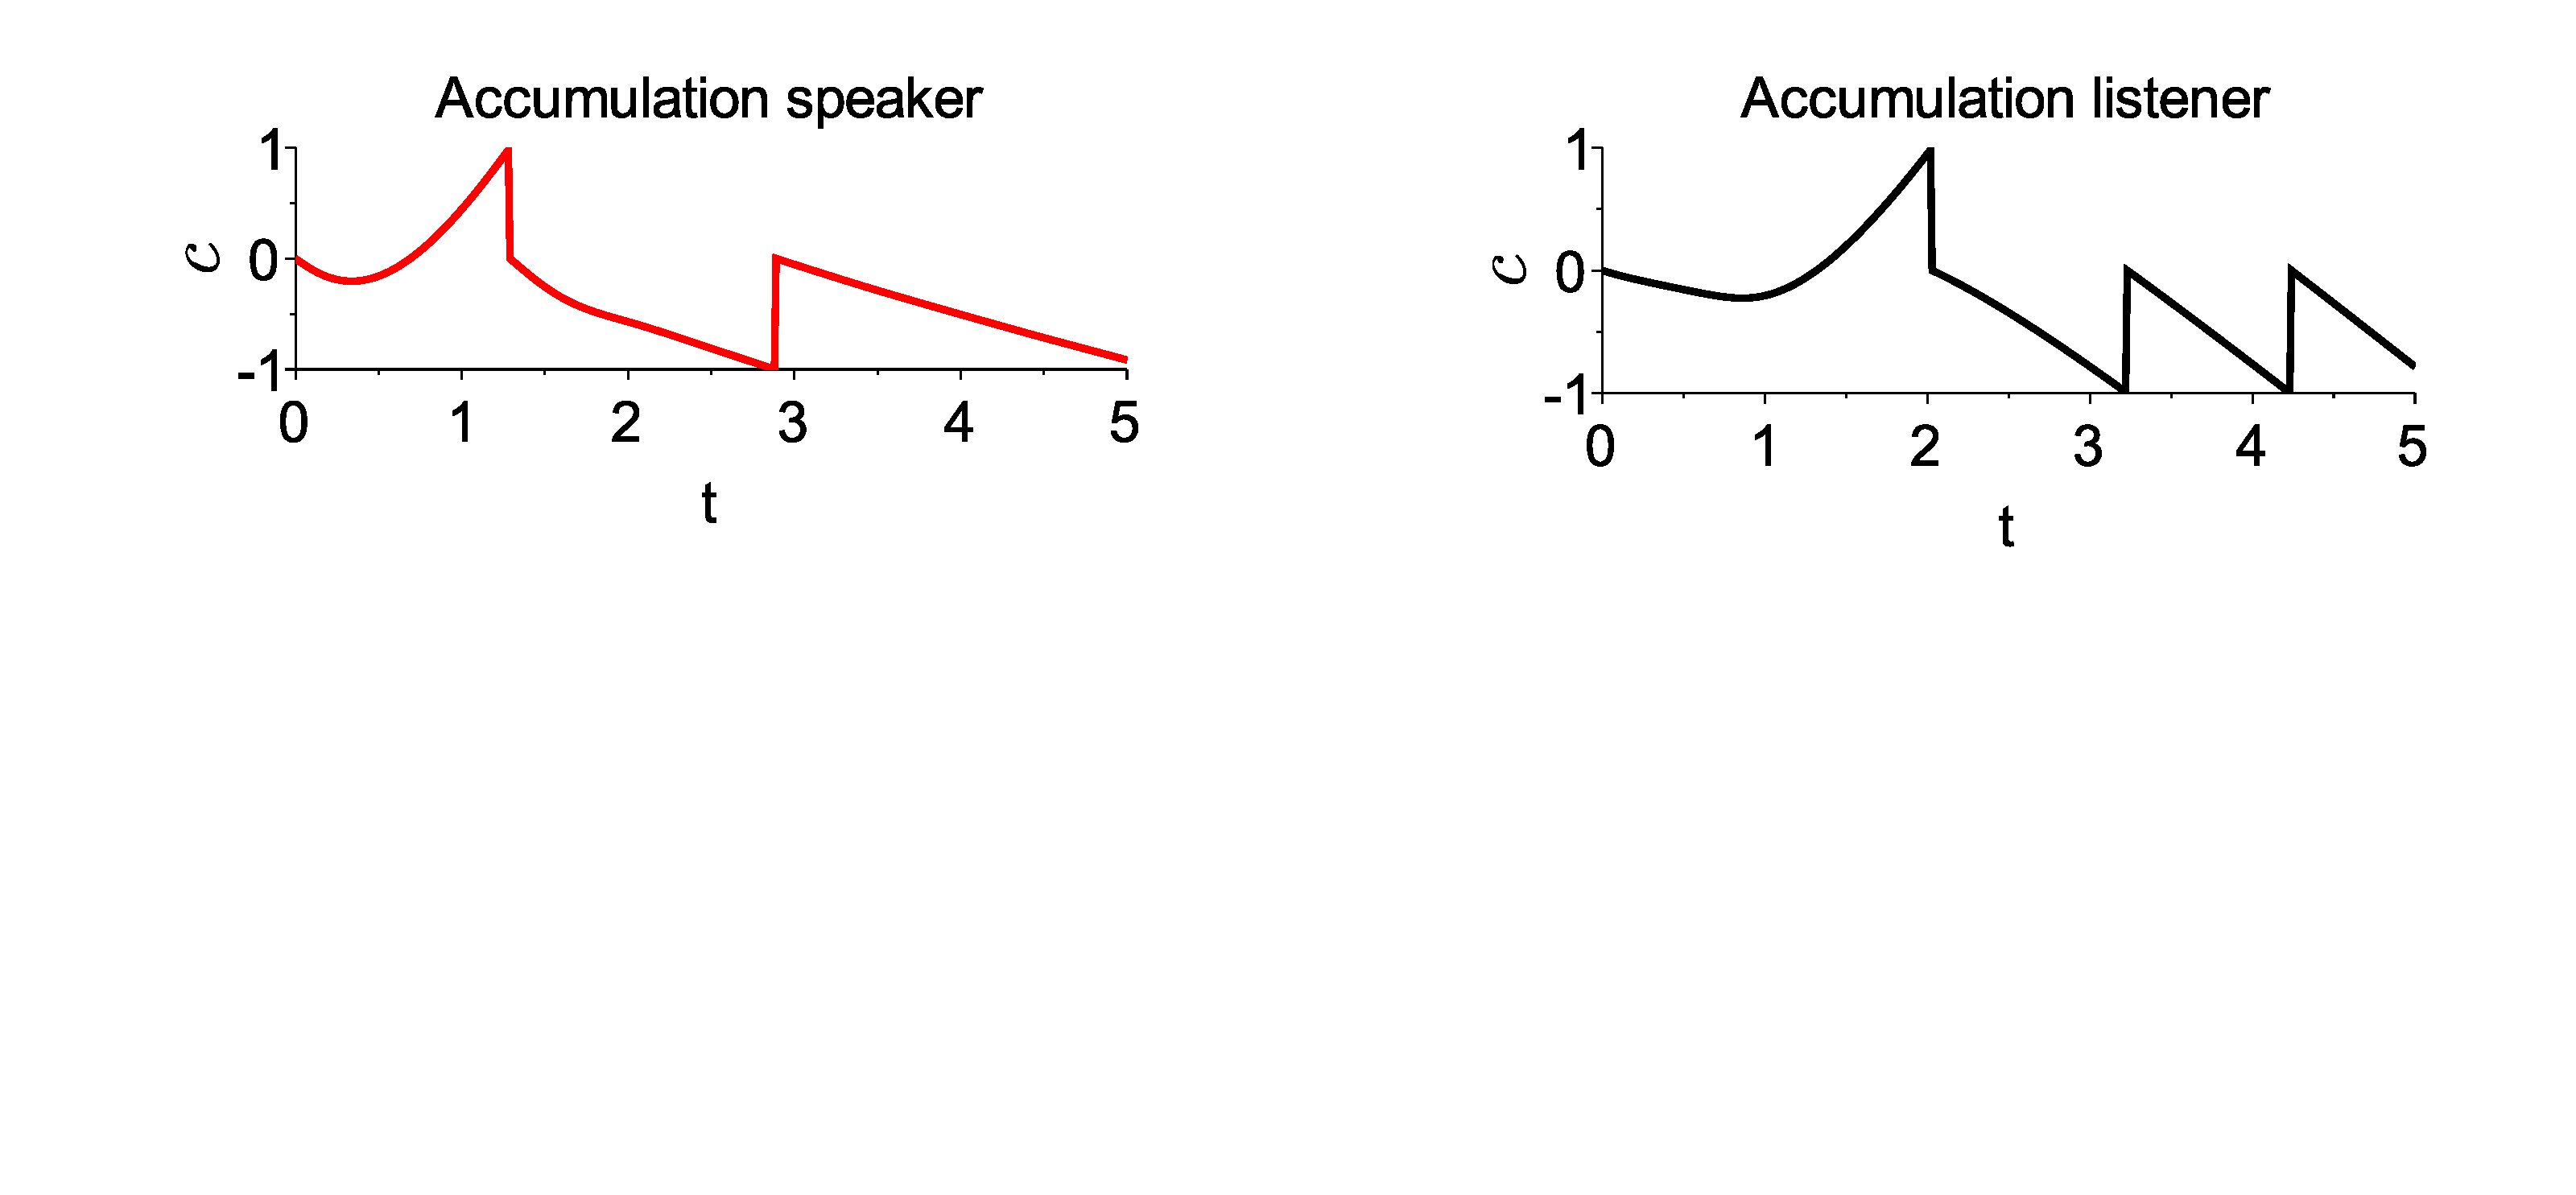
\includegraphics[width=\linewidth]{figure/smooth-transition_accumulation_small.pdf}
  \caption{Time series of the accumulation values $\gamma$ for the two agents. Scenario S3.}
  \label{smooth_acc}
\end{figure}


In scenario S3, the current speaker had a strong motivation to become listener and the current listener a strong motivation to become speaker. Figures \ref{simu_smooth} shows how the agents modulated their prosodic and non verbal signal productions (here the loudness and the pitch of their voice, and their gaze direction). Figure \ref{smooth_acc} shows the dynamic of the perceptual decision-making process. As one could expect, the model led to a short non conflicting overlap, in the terms given by \citep{schegloff_overlapping_2000}. 

Scenario S4 shown that if we modify the current speaker's motivation, we impact the behavior of the two agents. In S4, the current speaker had a strong motivation to go on speaking and the current listener a strong motivation to become the speaker. The result of this simulation is shown on Figure \ref{simu_interruption} and  Figure \ref{inter_acc}. In this situation, the model reproduced a conflicting overlap, which ended by the initial listener holding the floor.  

\begin{figure}
  \centering
  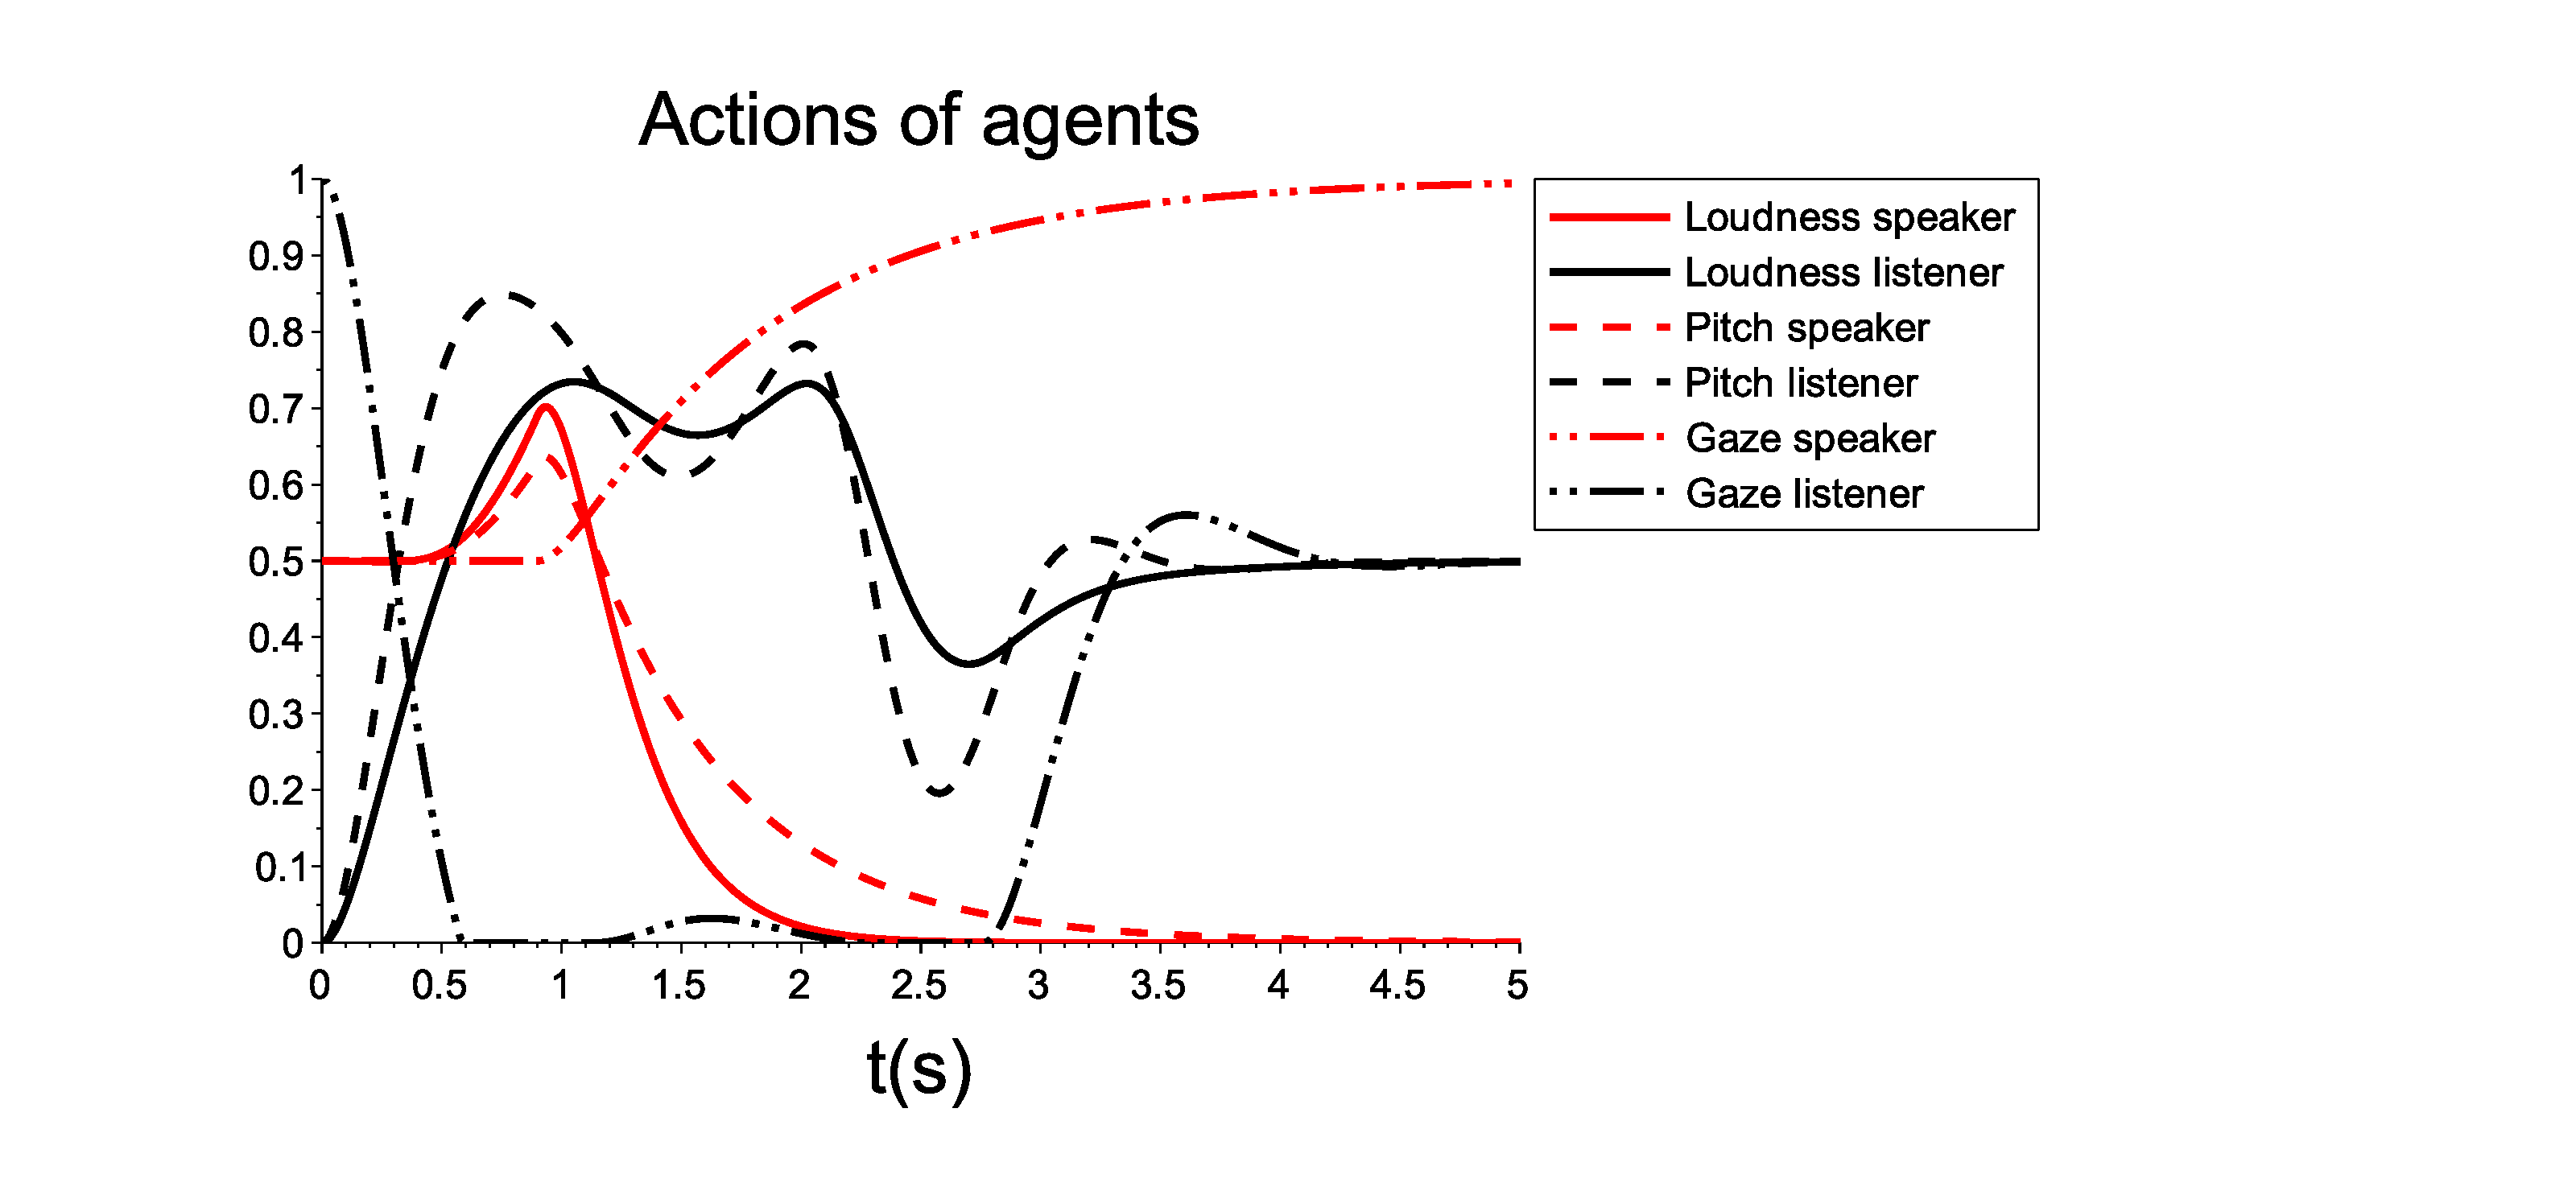
\includegraphics[width=\linewidth]{figure/emerg_sc1.pdf}
  \caption{Modulation of the prosodic and non verbal signals produced by the two agents. Scenario S4. The resulting behavior is a conflicting overlap lasting about 2 seconds.}
  \label{simu_interruption}
\end{figure}

\begin{figure}
  \centering
  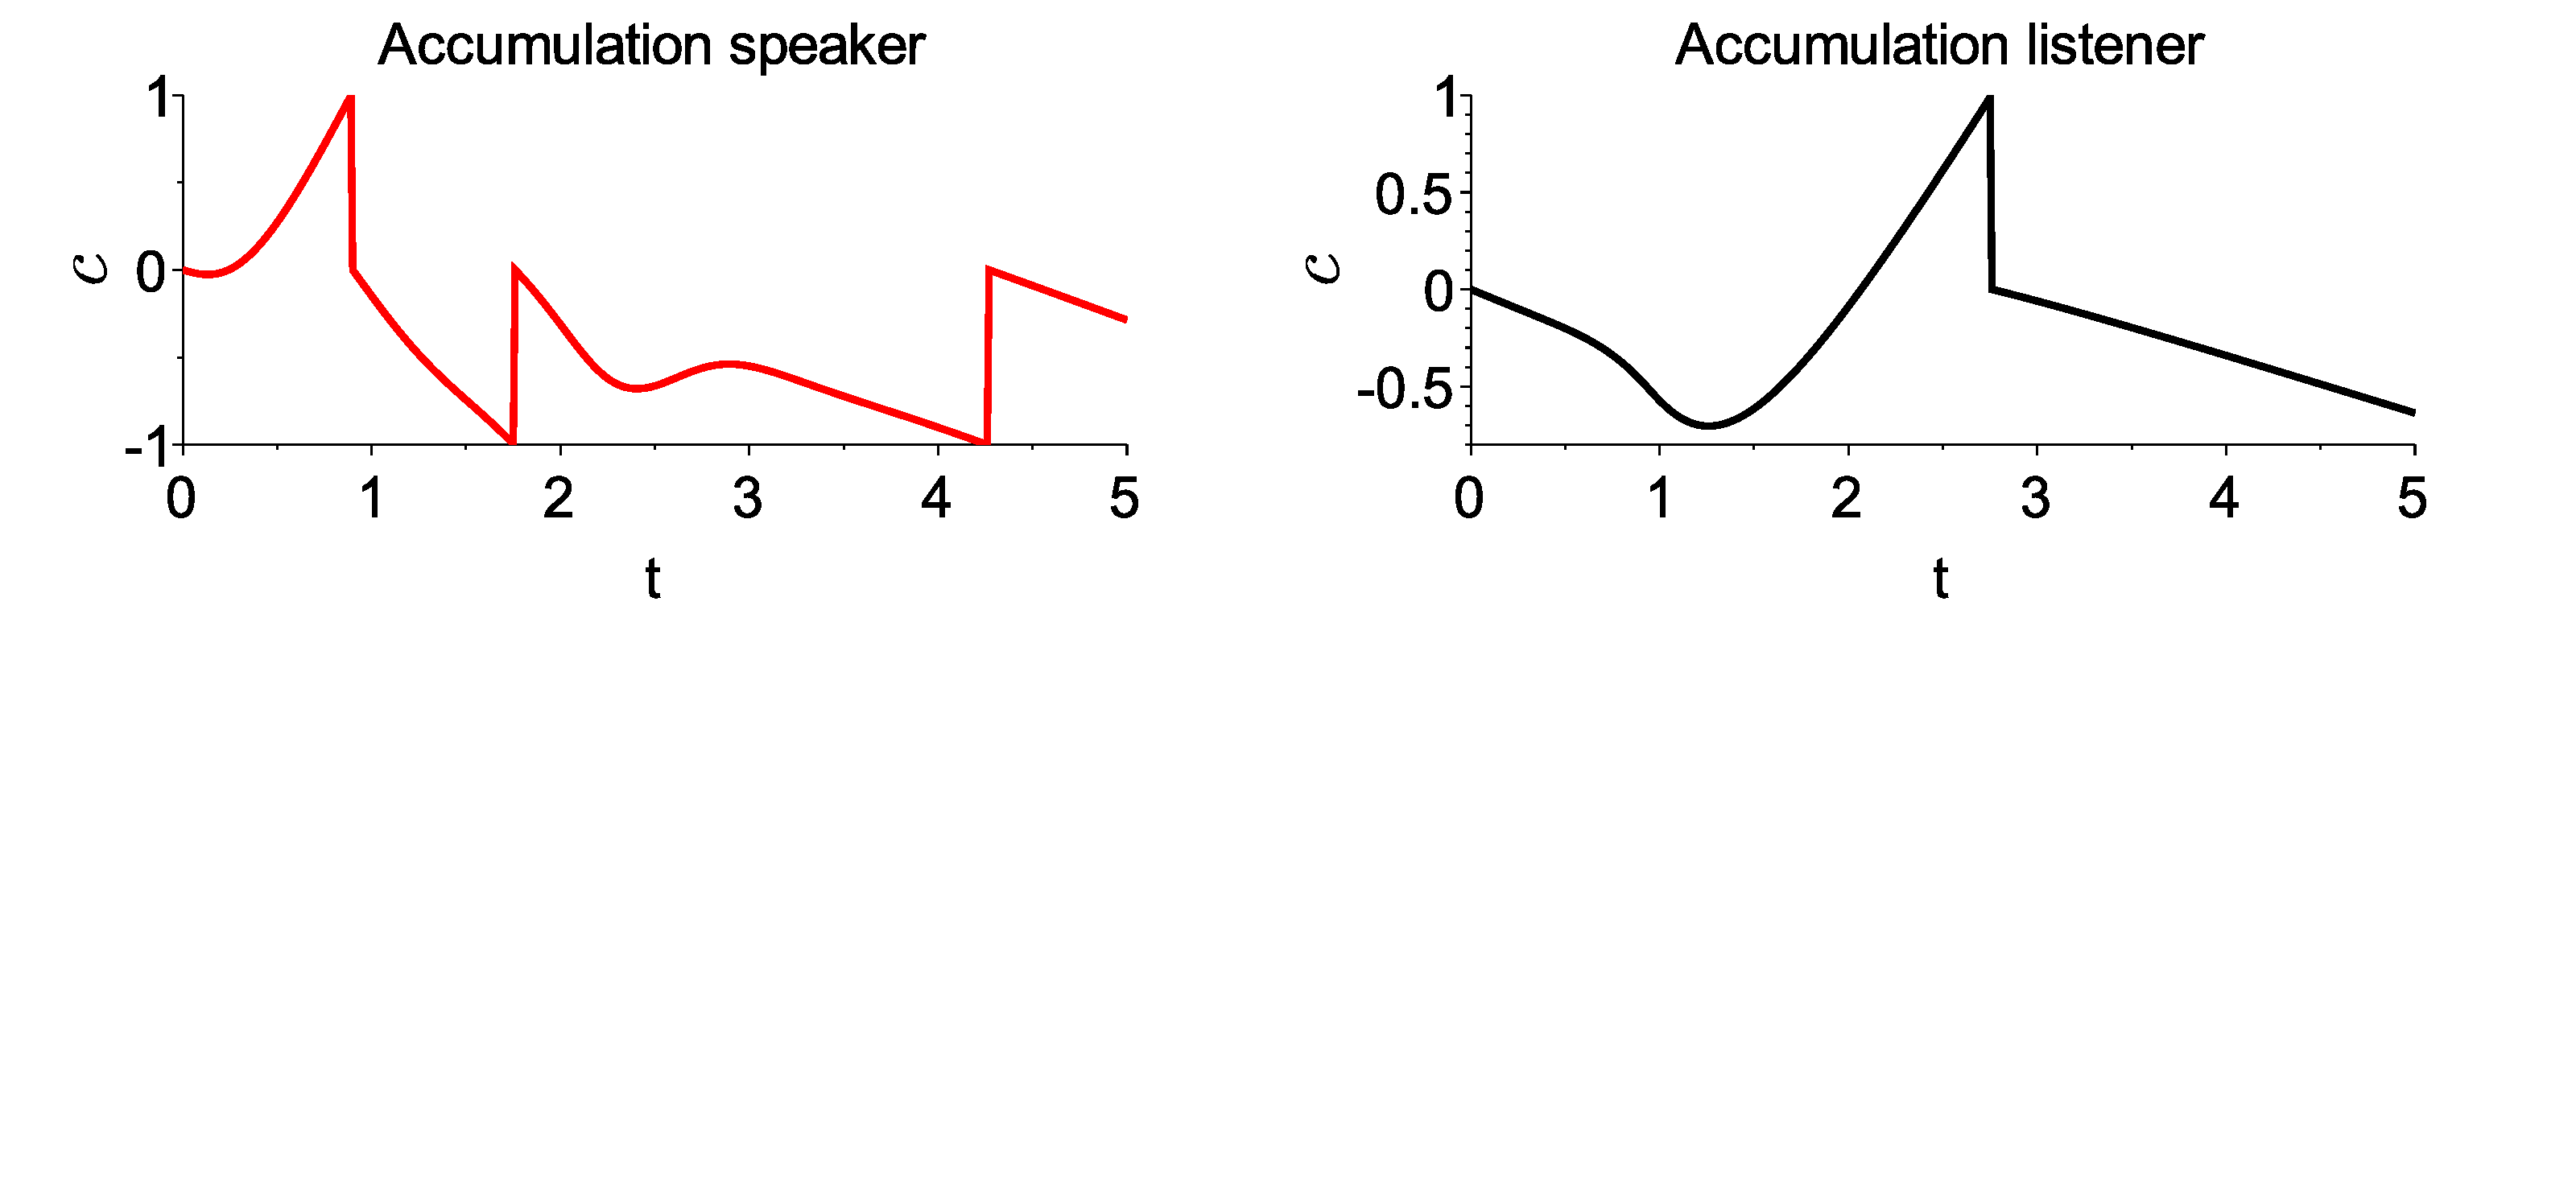
\includegraphics[width=\linewidth]{figure/acc_sc4_small.pdf}
  \caption{Time series of the accumulation values $\gamma$ for the two agents. Scenario S4.}
  \label{inter_acc}
\end{figure}

This scenario shows the continuous dependency of each participant to the signals production of the other one. At the beginning of the simulation, the current speaker was keeping its voice loudness to its mean value $0.5$. As its accumulation value raised, due to the raise in the loudness and pitch of the current listener, at $t\approx~750~\text{ms}$ the current speaker raised its own prosodic variables and averted its gaze, showing to the current listener its willingness to remain the speaker. Nevertheless, the modulations of the current speaker's signals (as defined by the equations governing the signal production) weakly impacted the signals production of the current listener. As a result, the current listener was continuing to try to grab the turn, the accumulation value of the current speaker crossed the positive threshold, and the current speaker finished to release the turn to the current listener. In turn, the current listener diminished its loudness and pitch, perceiving that the previous speaker finished to release the turn, which finally ended the conflictual situation.

If we now keep the same motivation value for the current speaker but we diminish the motivation of the current listener we obtain a completely different behavior for the two agents, as shown by Figures \ref{simu_buttin} and \ref{acc_buttin}, corresponding to scenario S5. We illustrate here the listener's successive but unsuccessful attempts to grab the turn. The choices made in the specific equations used for these simulations are responsible for the way the conflict is here resolved.  

\begin{figure}
  \centering
  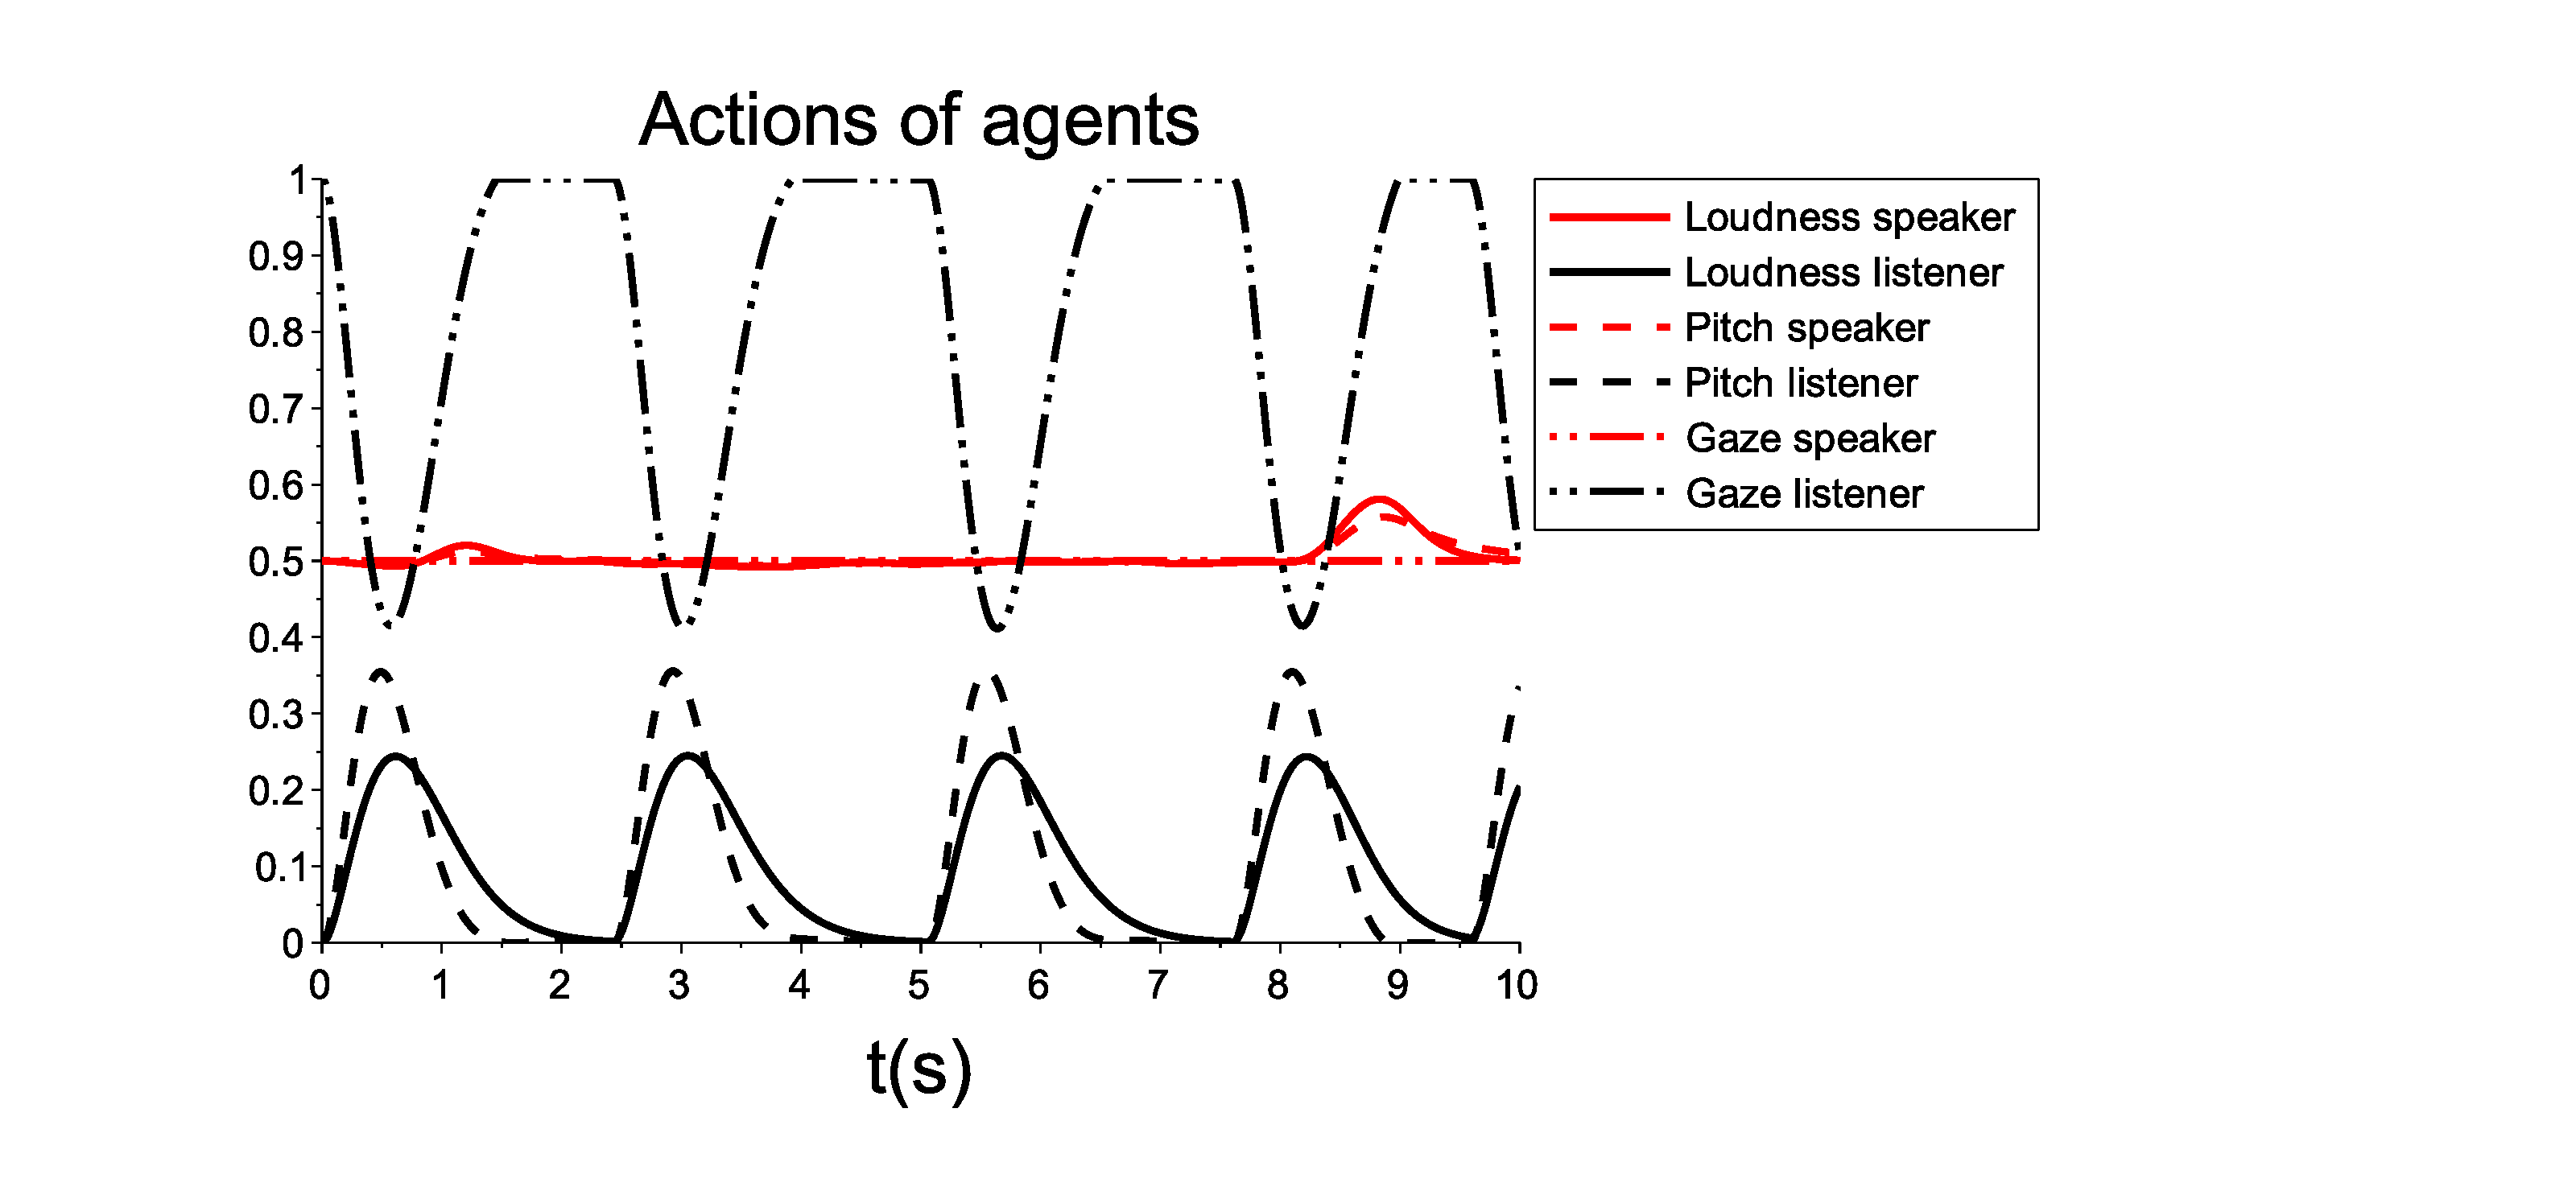
\includegraphics[width=\linewidth]{figure/emerg_sc2.pdf}
  \caption{Modulation of the prosodic and non verbal signals produced by the two agents. Scenario S5.}
  \label{simu_buttin}
\end{figure}

\begin{figure}
  \centering
  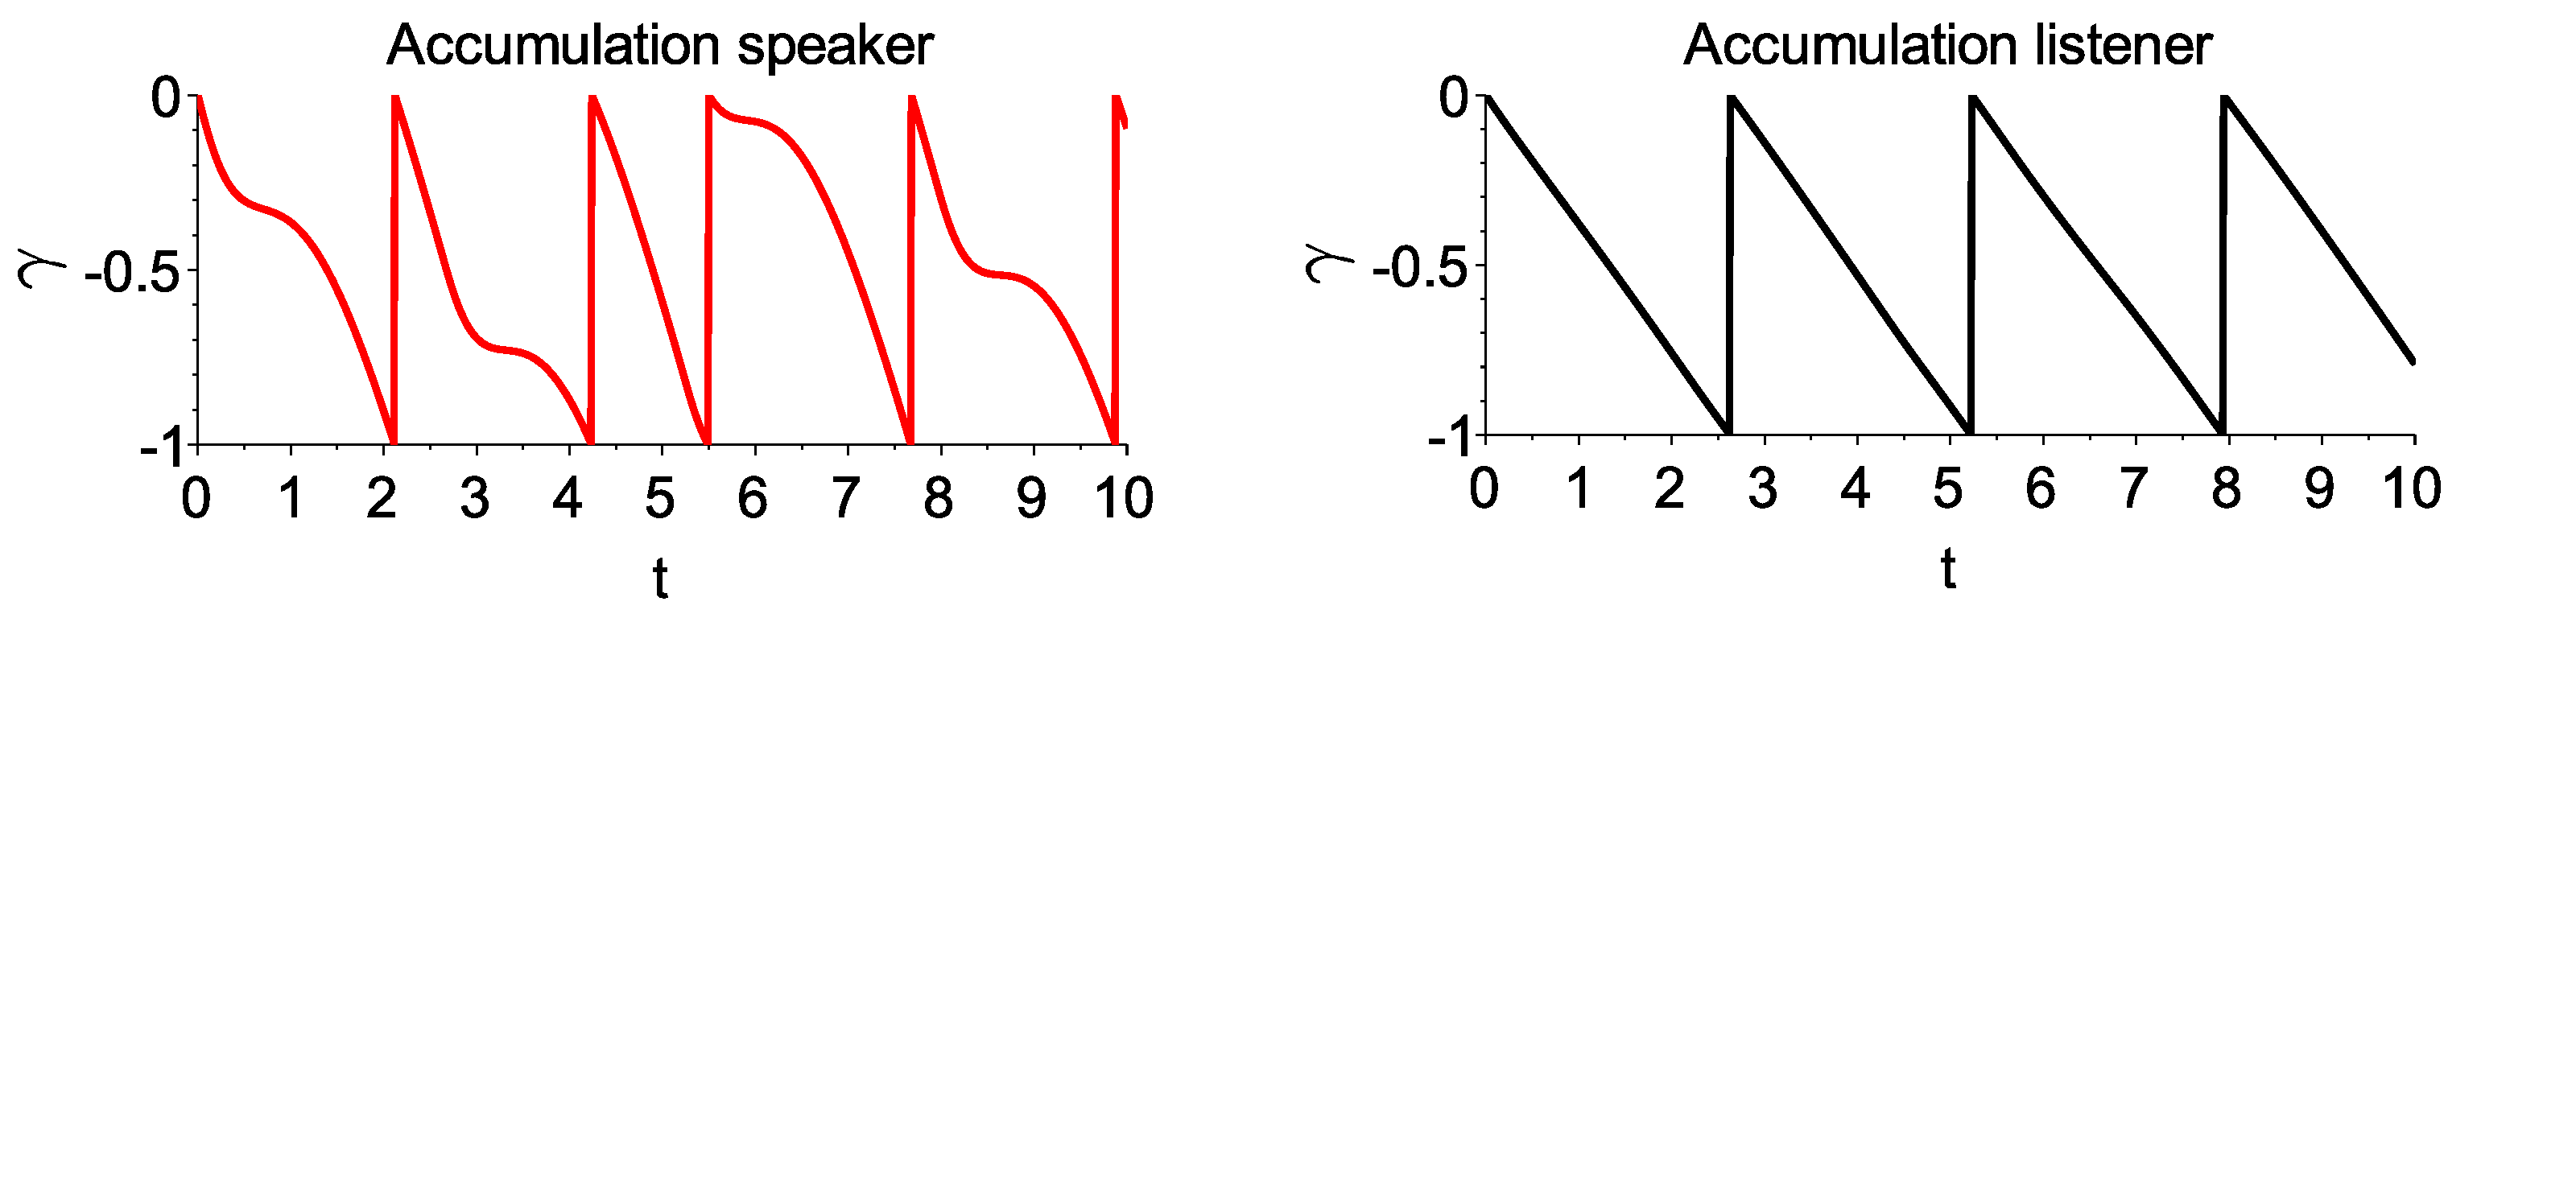
\includegraphics[width=\linewidth]{figure/acc_sc2_small.pdf}
  \caption{Time series of the accumulation values $\gamma$ for the two agents. Scenario S5.}
  \label{acc_buttin}
\end{figure}

In S5, the current speaker succeeded to keep its role in spite of the several turn-taking attempts of the current listener. This was because the motivation of the current listener was weaker than previously, meaning that it gave up more rapidly when it observed no cues indicating that the current speaker was releasing the turn. At the beginning of the simulation, the accumulation value of the current speaker raised, resulting in a current speaker averting its gaze from the listener. As the current listener gave up, the accumulation value of the current speaker diminished again, resulting in a gaze control parameter returning to the value $s_g=1$, meaning that the agent was fixing its partner. The fact that the loudness and pitch did not vary was simply due to an accumulation that was not high enough for the prosodic signals to raise. In other terms, the agent did not need to raise its prosodic signals to prevent the current listener to grab the turn. The observed repetition of the turn-taking attempts of the current listener was due to the fact that, as defined in section \ref{mod_pres}, when the accumulation value crosses the negative threshold, the accumulation process is reinitialized. Thus the current listener became again uncertain about the behavior of the current speaker, and thus initialized a new turn-taking attempt. 


These three simulations show that the resulting behavior of each participant is not solely determined by their motivation value, but is also indirectly impacted by the motivation of the other participant. In this sense, a sensorimotor coupling is established between participants, as the action variations of one participant directly impact the modulation of the actions of the other participant, resulting in a very versatile coordination. Since both participants continuously influence the other's behavior, one cannot predict in advance the resulting behavior of the two participants. These behaviors are then an emergent property of the interaction of the two participants. 

\subsection{Adaptability of the behavior}

The behaviors of the two participants emerge from the interaction. But, what benefits bring this sensorimotor coupling between both participants?
We show in this section, how this sensorimotor coupling can explain how participants can seamlessly adapt to different environmental settings without modifying the different equations governing the perceptual decision-making process and the production of the prosodic and non verbal signals. We will show this adaptability on examples where we varied the number of signals the agents can perceive. 

% ------------------------------------------------------------------------------
%\subsubsection{Adaptability to the amount of information}

The different analyses conducted in this section have been performed using scenario S5 (see table \ref{tab_scenarios_emergence}) and a variant S6, where the agents did not use the direction of gaze of their partner in the perceptual decision-making process. 
These two scenarios correspond to a conflicting situation when the current listener makes several unsuccessful attempts to grab the turn, the current speaker averting its gaze in response to the turn-grabbing attempt. Figure \ref{simu_buttin} illustrates the signal production of the two participants when they perceived the totality of the signals produced by the other participant (S5). Figure \ref{adapt_nogaze} illustrates what happened when agents did not have access to the gaze direction of their partner (S6).

% \begin{figure}
%   \centering
%   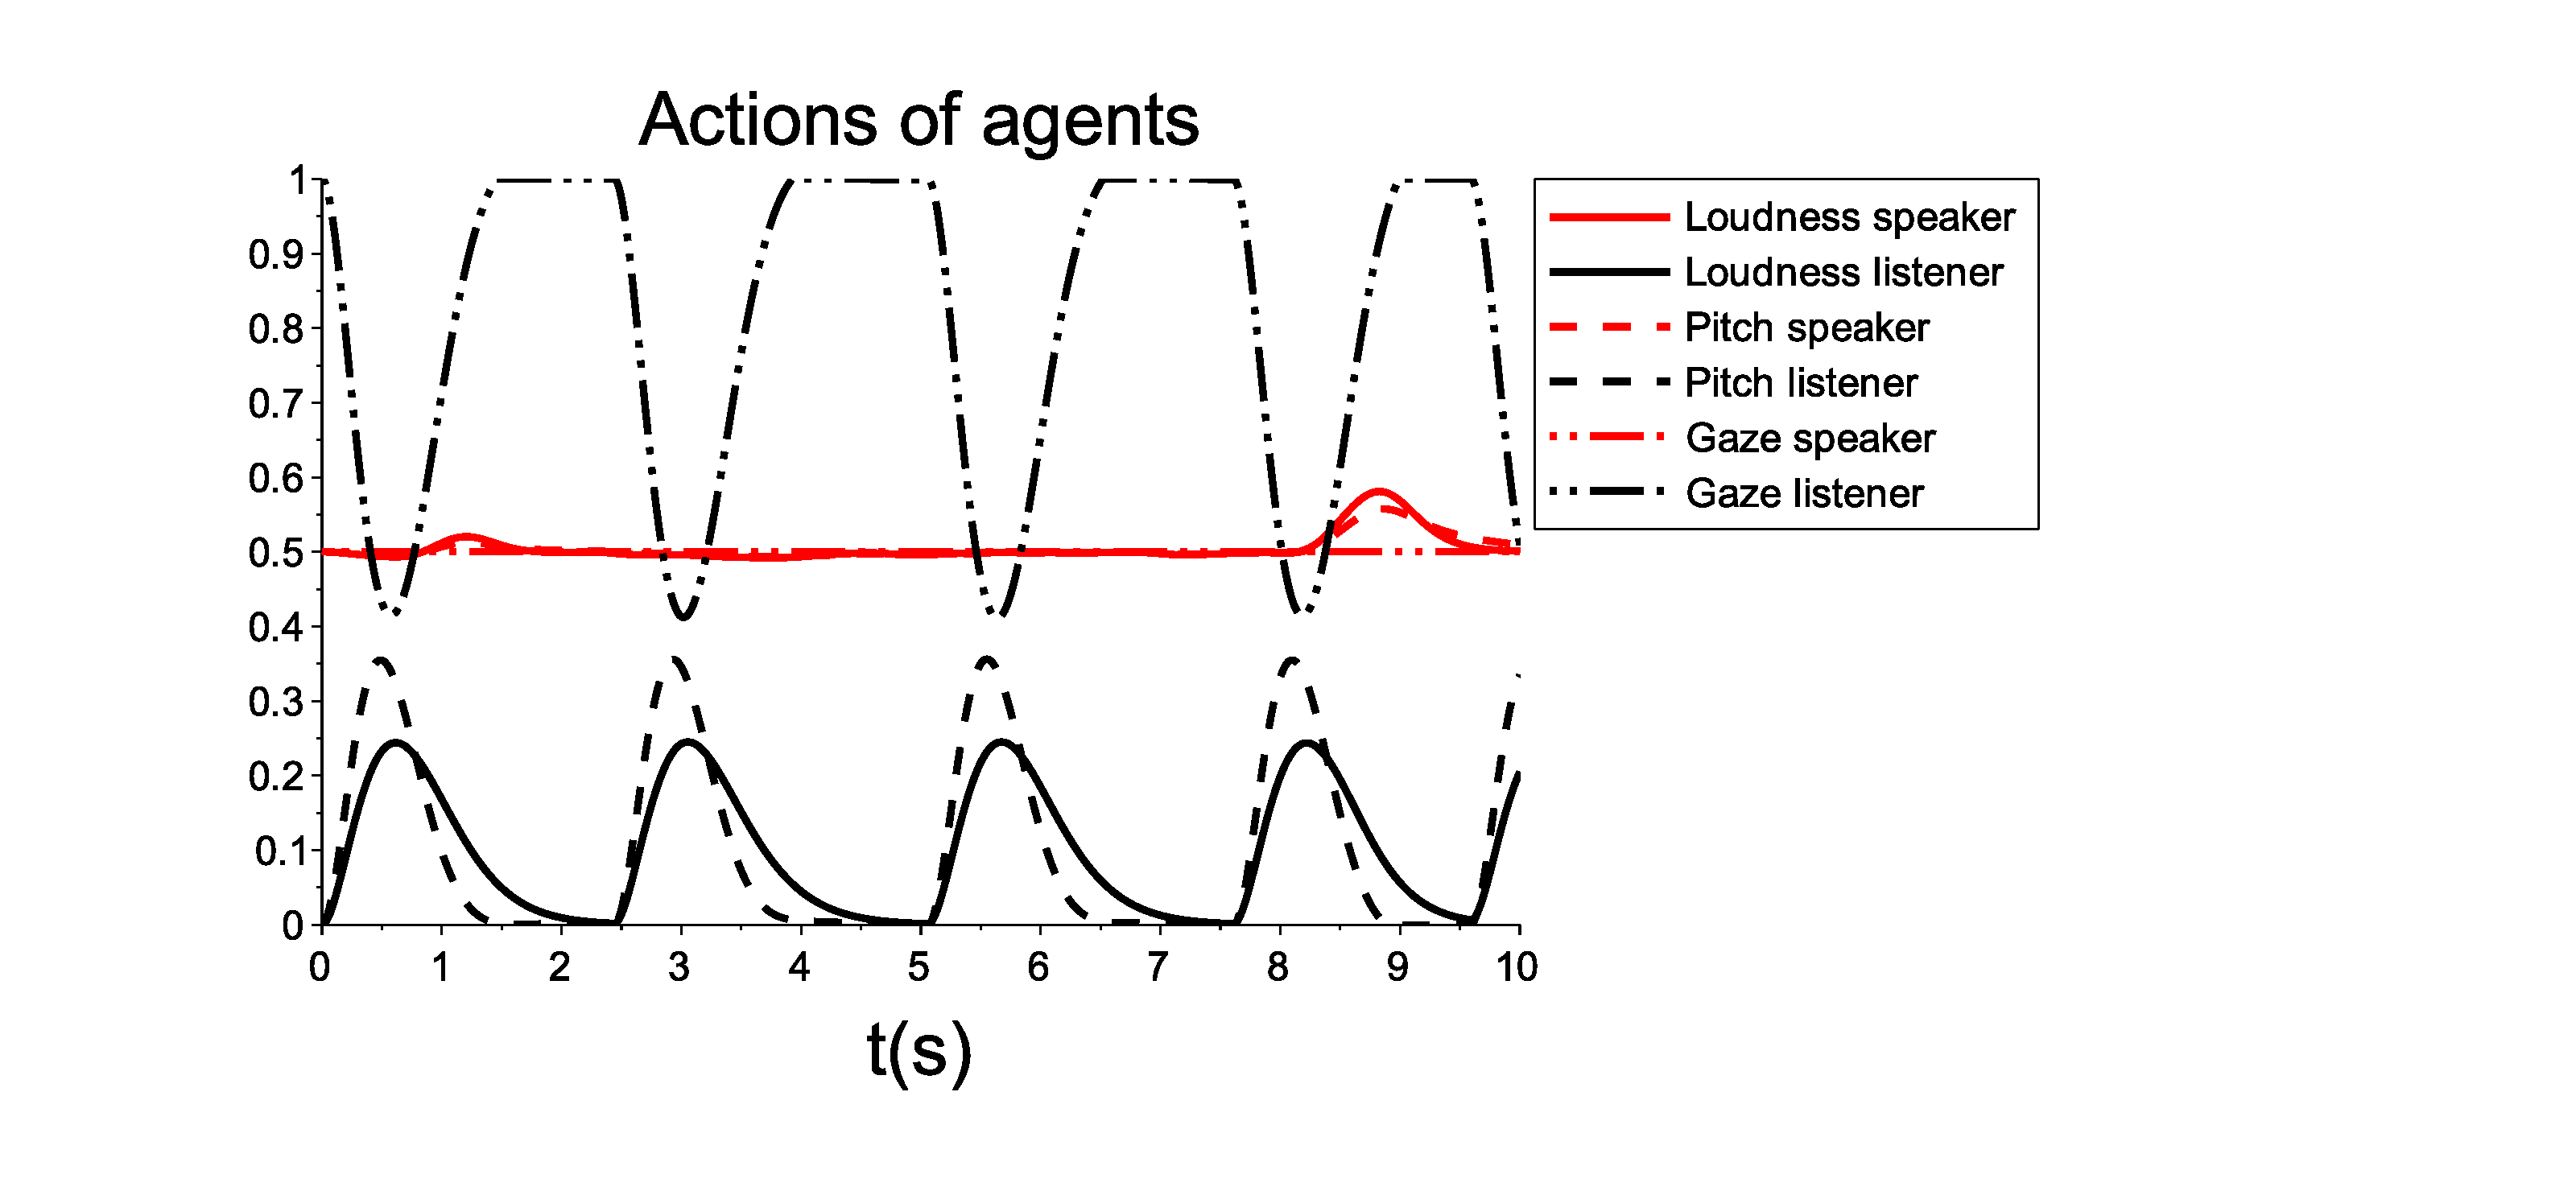
\includegraphics[width=\linewidth]{figure/adapt_all.pdf}
%   \caption{Conflictual situation where the participants have access to all of the three signals produced by the other participant.}
%   \label{adapt_all}
% \end{figure}

%We then analyzed the behavior of the participants when they could not perceive the gaze direction of their partner and had only access to the vocal modalities of the other participant's behavior.

\begin{figure}
  \centering
  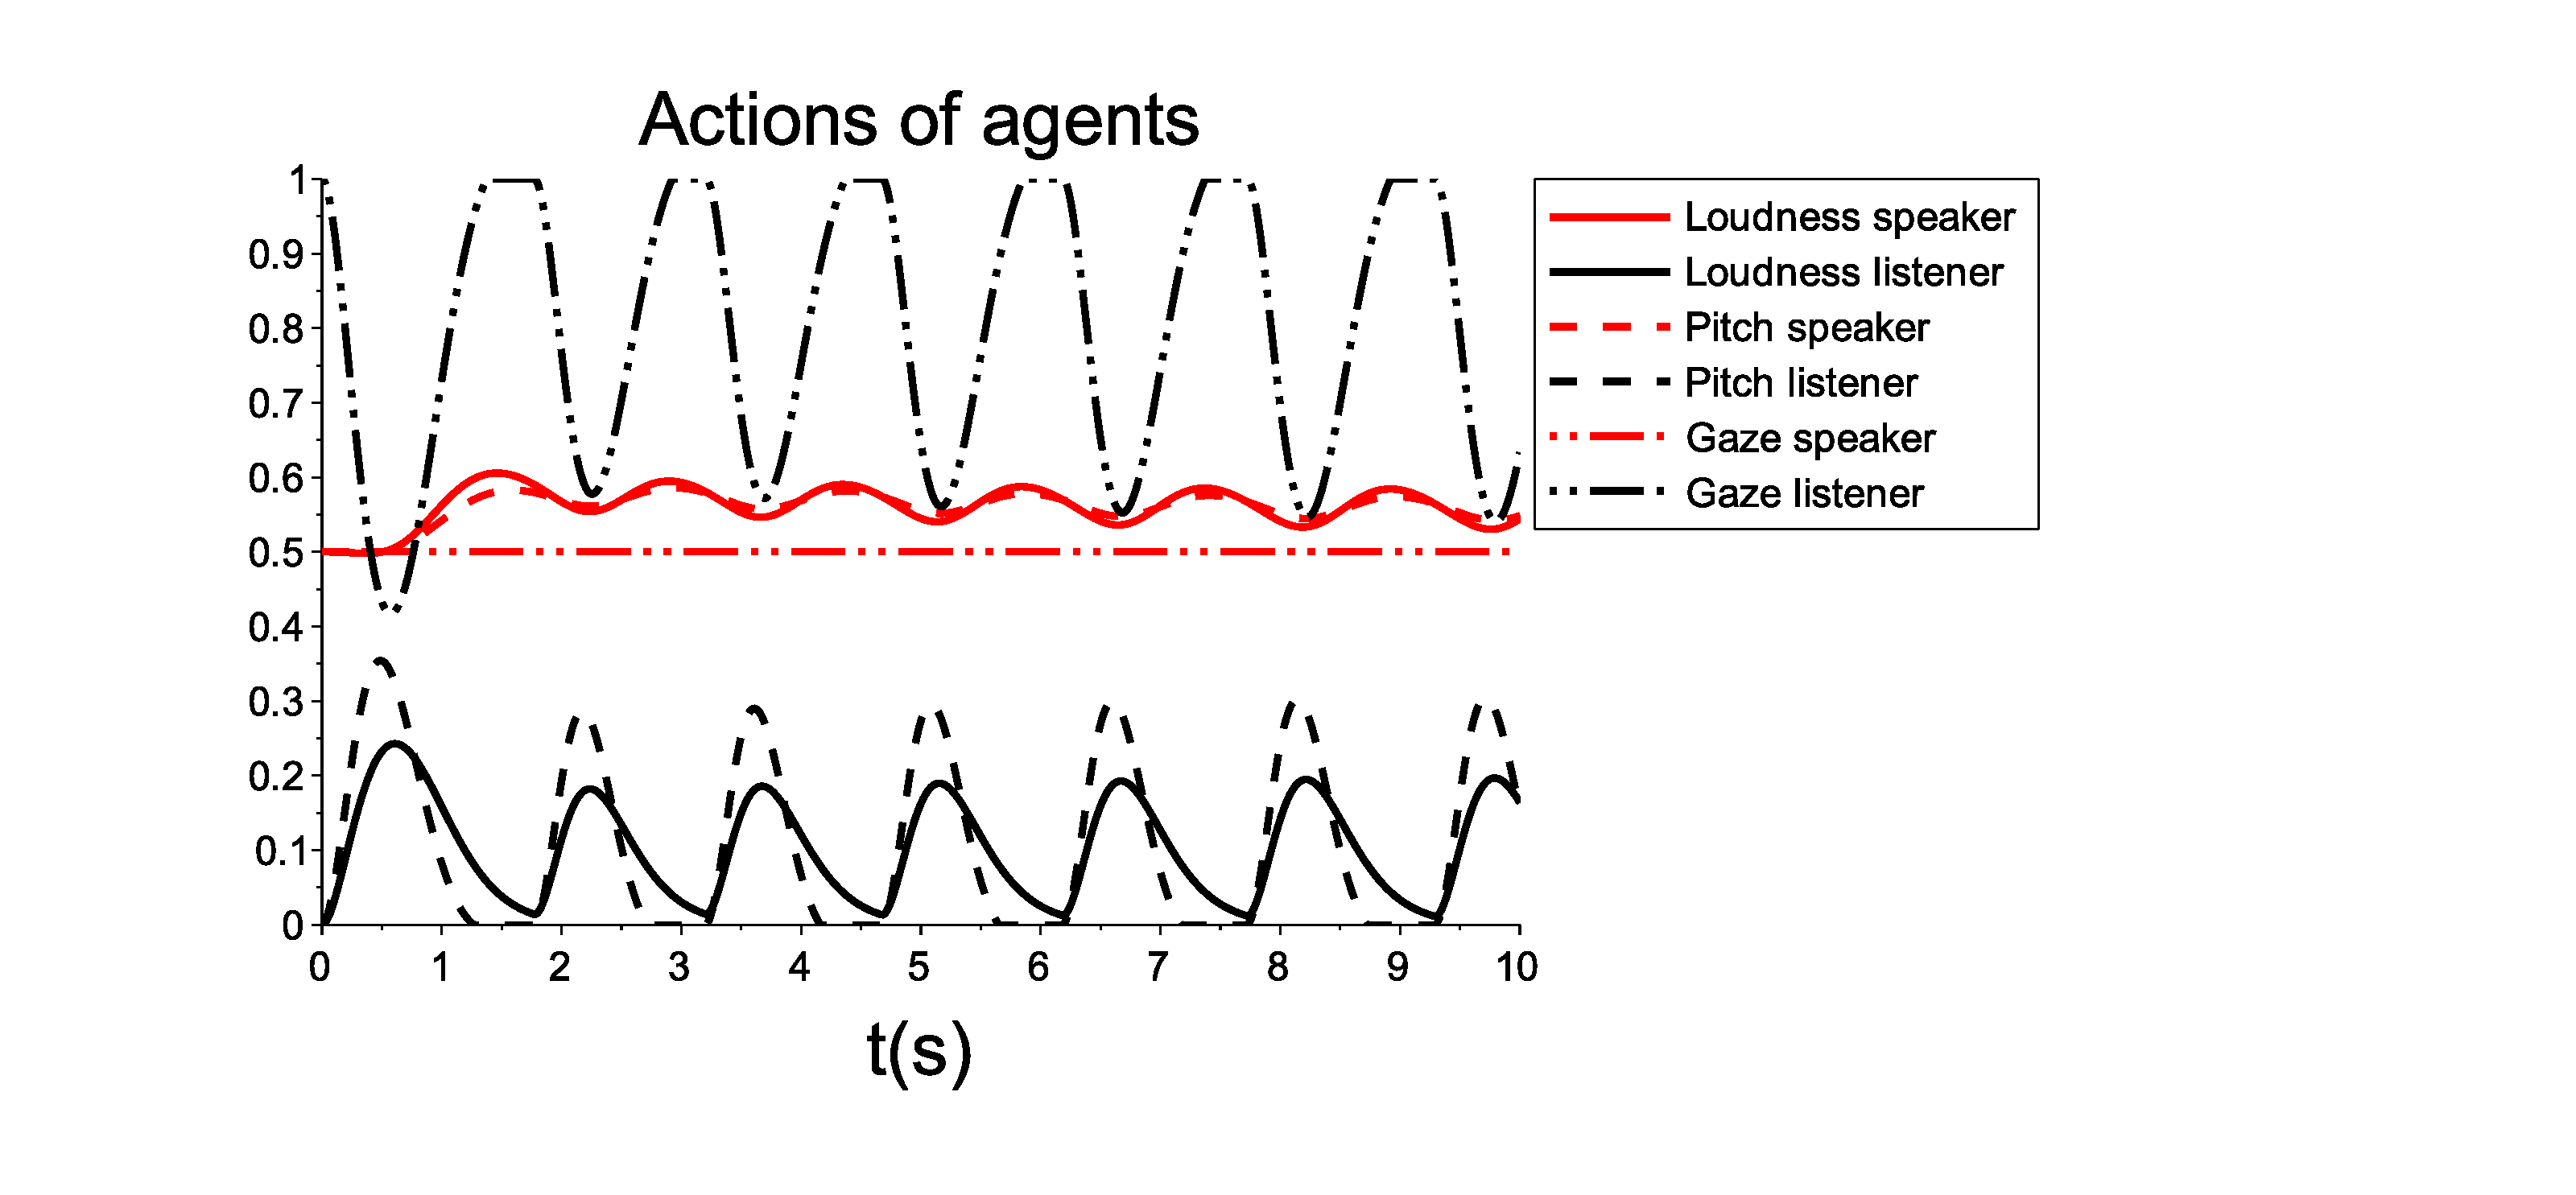
\includegraphics[width=\linewidth]{figure/adapt_nogaze.pdf}
  \caption{Conflictual situation where the participants do not have access to the gaze information of the other participant. Scenario S6.}
  \label{adapt_nogaze}
\end{figure}

%As shown on Figure \ref{adapt_nogaze}, 
%During S6, we observed a raise in the prosodic signals of the speaker. This was due to the joint influence of the volume and pitch raises of the listener, and to the current accumulation value, linked to the absence of the gaze information. 
In scenario S5, where participants exchanged the whole set of signals, the speaker's accumulation value raised but remained negative as the current listener attempted to grab the turn but rapidly gave up. It was because the information conveyed by the listener's gaze evolved slowler than the prosodic information. Thus, at the beginning, the speaker did not perceive the cue in the gaze information indicating that the listener wanted to grab the turn, diminishing consequently the variation of the accumulation value. 

In scenario S6, the accumulation value of the listener raised more rapidly and took more time to diminish in response to the lack of cues indicating that the speaker released the turn, resulting in a an agent raising more and longer its loudness and pitch. The fact that the loudness and pitch of the listener raised more impacted also the accumulation value of the speaker that raised more and became positive, that was not the case previously, resulting in an agent that raised more its own loudness and pitch. This raise impacted the accumulation value of the listener that diminished again, resulting in the listener giving up its turn-taking attempt. 

In addition, we simulated a situation where the participants perceived only the voice loudness, and we observed the same kind of adaptation: the speaker raising even more its loudness in response to the turn-taking attempts of the listener, as shown on Figure \ref{adapt_volume}.

\begin{figure}
  \centering
  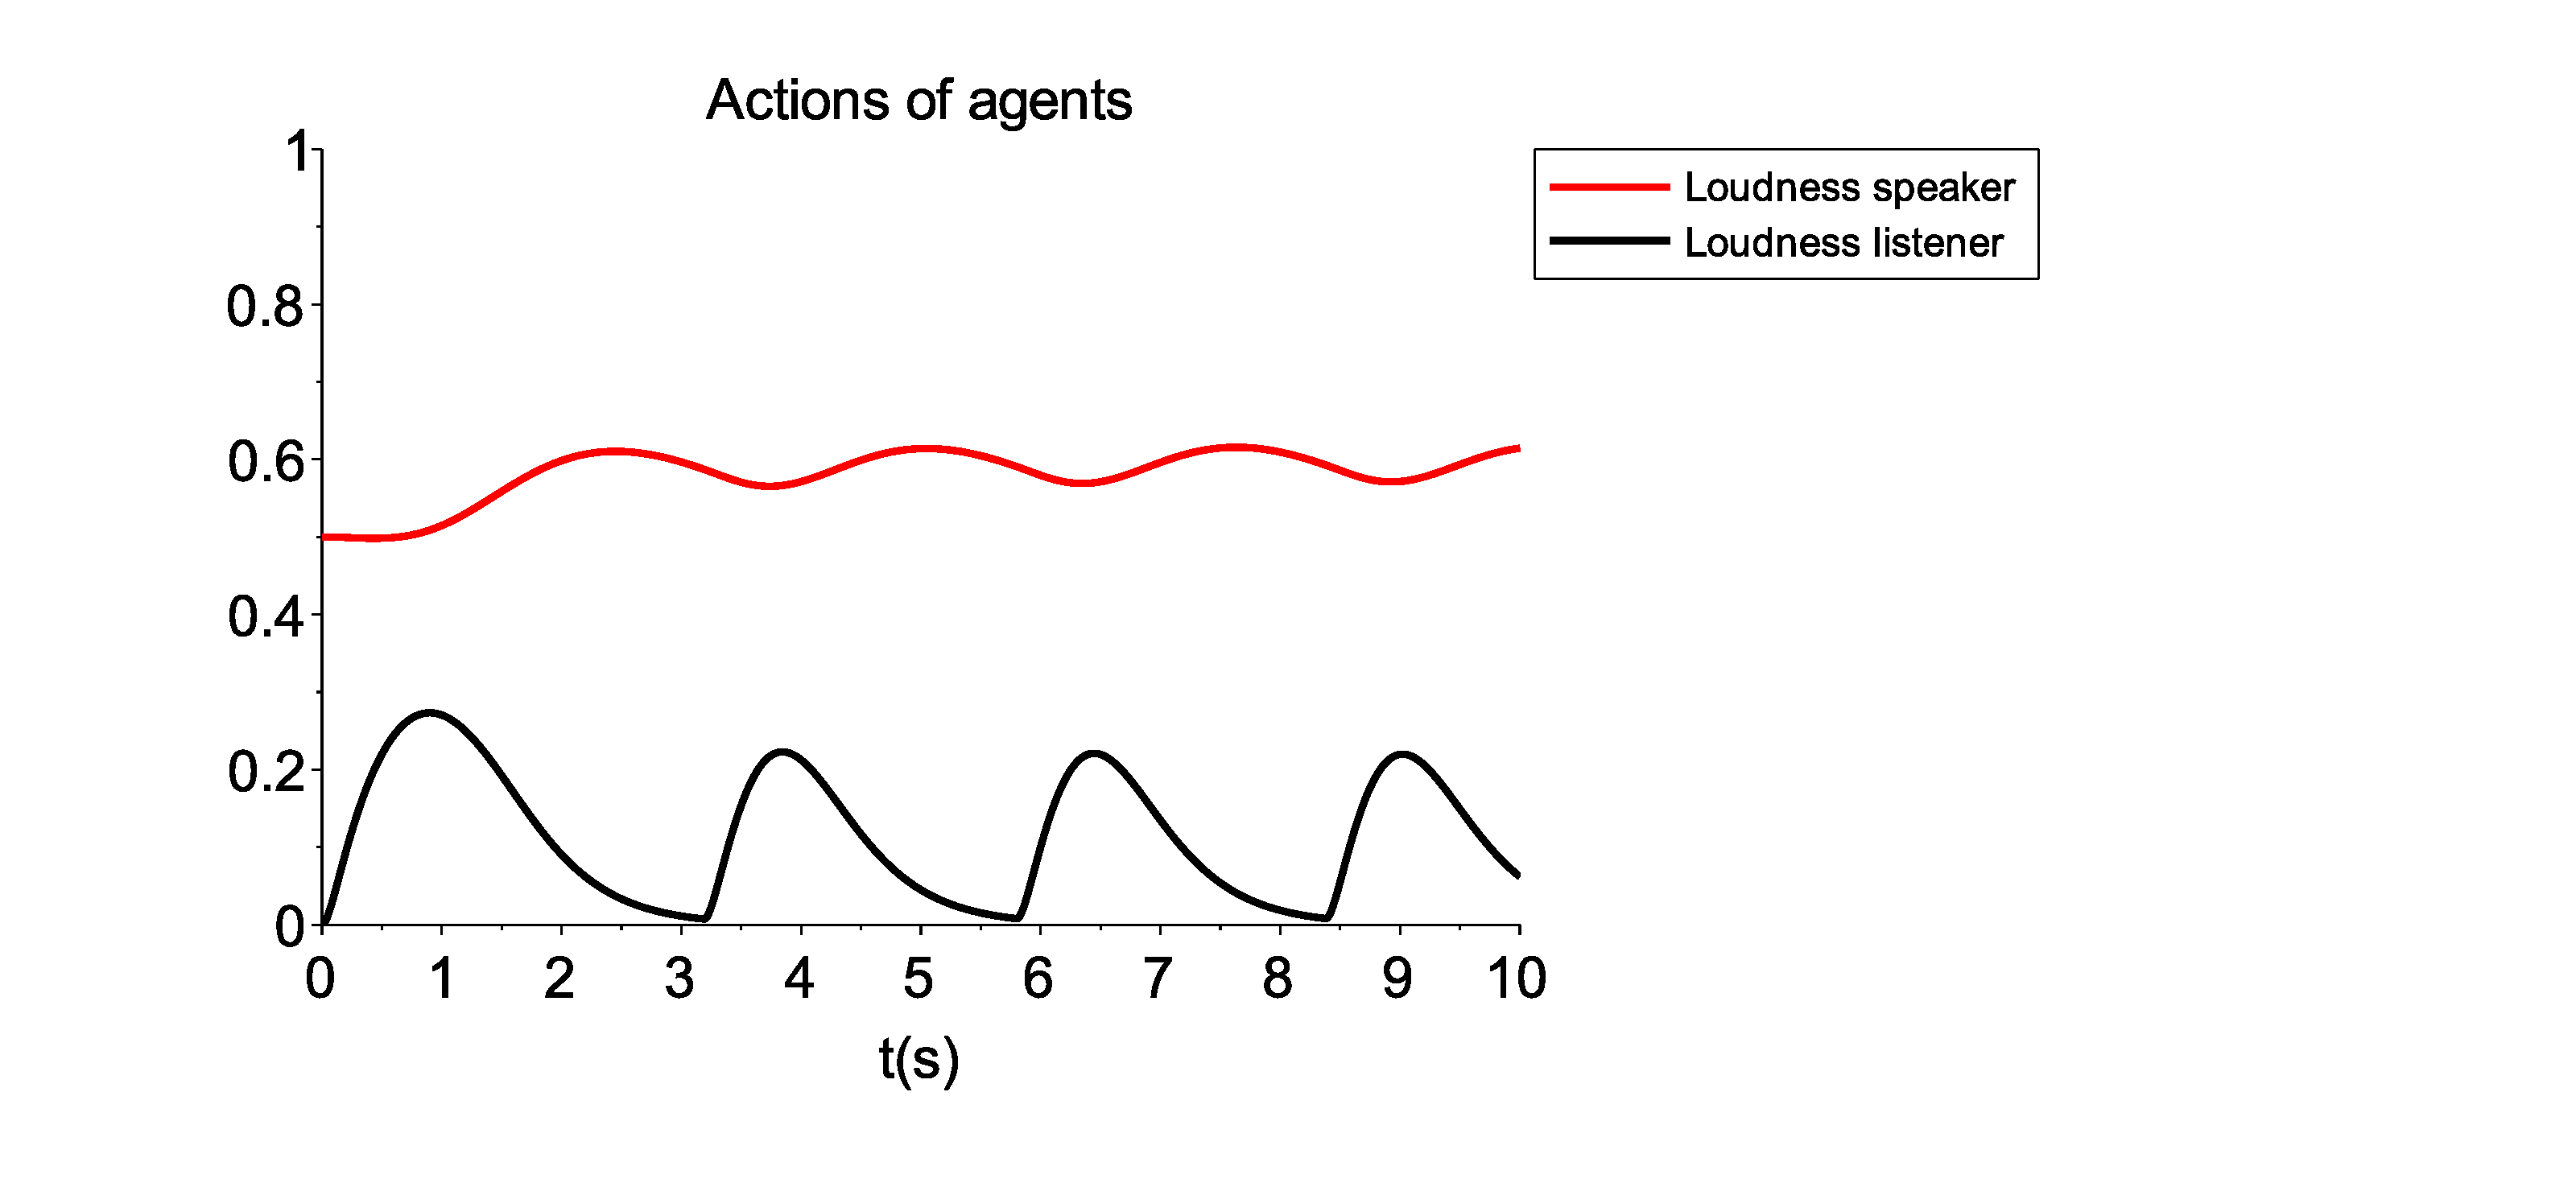
\includegraphics[width=\linewidth]{figure/adapt_volume.pdf}
  \caption{Conflictual situation where the participants have access only to the loudness produced by the other participant.}
  \label{adapt_volume}
\end{figure}

What is remarkable about these three contrasting scenarios is that the conflict durations did not vary significantly with the amount of signals handled by the agents. Interestingly, participants kept the coordination effective, and this was not totally due to the equations we formulated, but also to the manner participants varied their signals, accentuating their signal productions to compensate the lack of information in the environment. The adaptation of the agents is thus an emergent property of the interaction. Such mechanism is a great advantage for a turn-taking model between the agent and the user, as the adaptation of the agent is naturally done in the course of the interaction, without needing an explicit adaptation algorithm. Nevertheless, having the same adaptation properties in user-agent interactions necessitates that the user can also actively adapt to the situation. We explore this point in Section \ref{sec:eval}.

\section{Implementation of the model}
\label{impl}

% Expliquer BMLA (au moins faire référence au fait que c'est une extension)

\subsection{Requirements}

%We want an agent able to coordinate its turn in real-time with the user in a real dialogue scenario. In this kind of interaction, 
Turn-taking management is one of the many processes an ECA has to manage to be engaged in a natural interaction with the user. 
Among others, turn-taking management is closely linked with 
the dialog management, including natural language understanding and generation \citep{skantze_towards_2010}, 
the grounding which necessitates to generate, and to react, to the different types of feedback the user may produce, such as backchannels \citep{kopp_dynamic_2014,bevacqua_multimodal_2010}, 
and also the control of the engagement process with the user (see \cite{clavel_fostering_2016} for a review about engagement). 
Existing ECA architectures provide the core functionalities required to support these processes, at least partially. 
Our aim was to propose a solution for integrating our model into existing ECA architecture.
However, the continuous nature of the two main components of the model that are executed in parallel, implies some adaptations of existing architectures. 

%and to bring a stone to the buiding of ECA able to sustain mixed initiative dialogue in a very human-like fashion. 

%For example, apart from the turn-taking coordination, the agent has to be able to interpret the utterance of the user, formulated in natural language, and to generate an utterance in response, managing grounding by interpreting and generating the different types of feedback the user can produce, such as backchannels, perceiving the engagement of the user or showing its own engagement in the dialogue. 
%In order to manage the concurrent execution of all these processes, we would like to use an existing modular architecture, where we could integrate our turn-taking model without adapting it to work with the other components of this architecture.

%On the contrary, our model perceives and controls the actions of the agent in a continuous fashion : actions of the agent are continuously modulated rather than triggered by decision modules, and the perception and decision processes run concurrently rather than sequentially. 
%These requirements follows the design principle of the recent architecture ASAP. 
%We thus chose the ASAP framework as a basis for the implementation of our model. 

The closest solution suitable for implementing our model is ASAP from \cite{kopp_architecture_2014}.
Nevertheless, some mandatory details lack in the specifications of the ASAP architecture. For instance, we have to manage the concurrent execution of the different decision modules. Indeed, several conflicting actions can be sent at the same time to the realizer, which thus requires a mechanism to select or merge the actions in order to avoid inconsistencies in the action generation. Another issue is the selection of the multimodal communicative actions corresponding to the commands provided by the decision modules, and specifically, how to handle commands that require to change in real-time the actions produced by the agent. 
%To address these issues we based our solution 
%We wanted also to specify more precisely the communication mecanism between the different modules.
We borrowed some principles from the Ymir architecture \cite{thorisson_mind_1999} to address these issues and thus we extended the ASAP architecture.  
%We will now describe our agent architecture.

\subsection{Architecture overview}

%We used the current repartition given by the ASAP architecture. 
The overall organisation of the BeAware architecture, which is composed of six modules, is similar to ASAP, as shown on Figure \ref{overall_archi}. 
Modules dedicated to the perception are: 
the Sensing module receiving sensory data, 
the Behavior Interpreter module, interpreting behavioral patterns, such as nodding, from the multimodal sensory data, 
and the Function Interpreter, interpreting the communicative functions of the behavioral patterns. 
The decision part is composed of three modules, 
the Intent Planner generating the communicative intentions of the agent, 
the Behavior Planner generating the multimodal actions from the communicative intentions and managing the execution of the actions (activating, modulating or interrupting the actions) based on the behavioral patterns perceived by the Behavior Interpreter,
and finally the Behavior Realizer. 
% COMMENT TODO: Pierre : Mathieu verifie les fonctions du behavior planner et du behavior realizer
% TODO: valider nom Behavior Interpreter (au lieu de Interpretation)

\begin{figure}
  \centering
  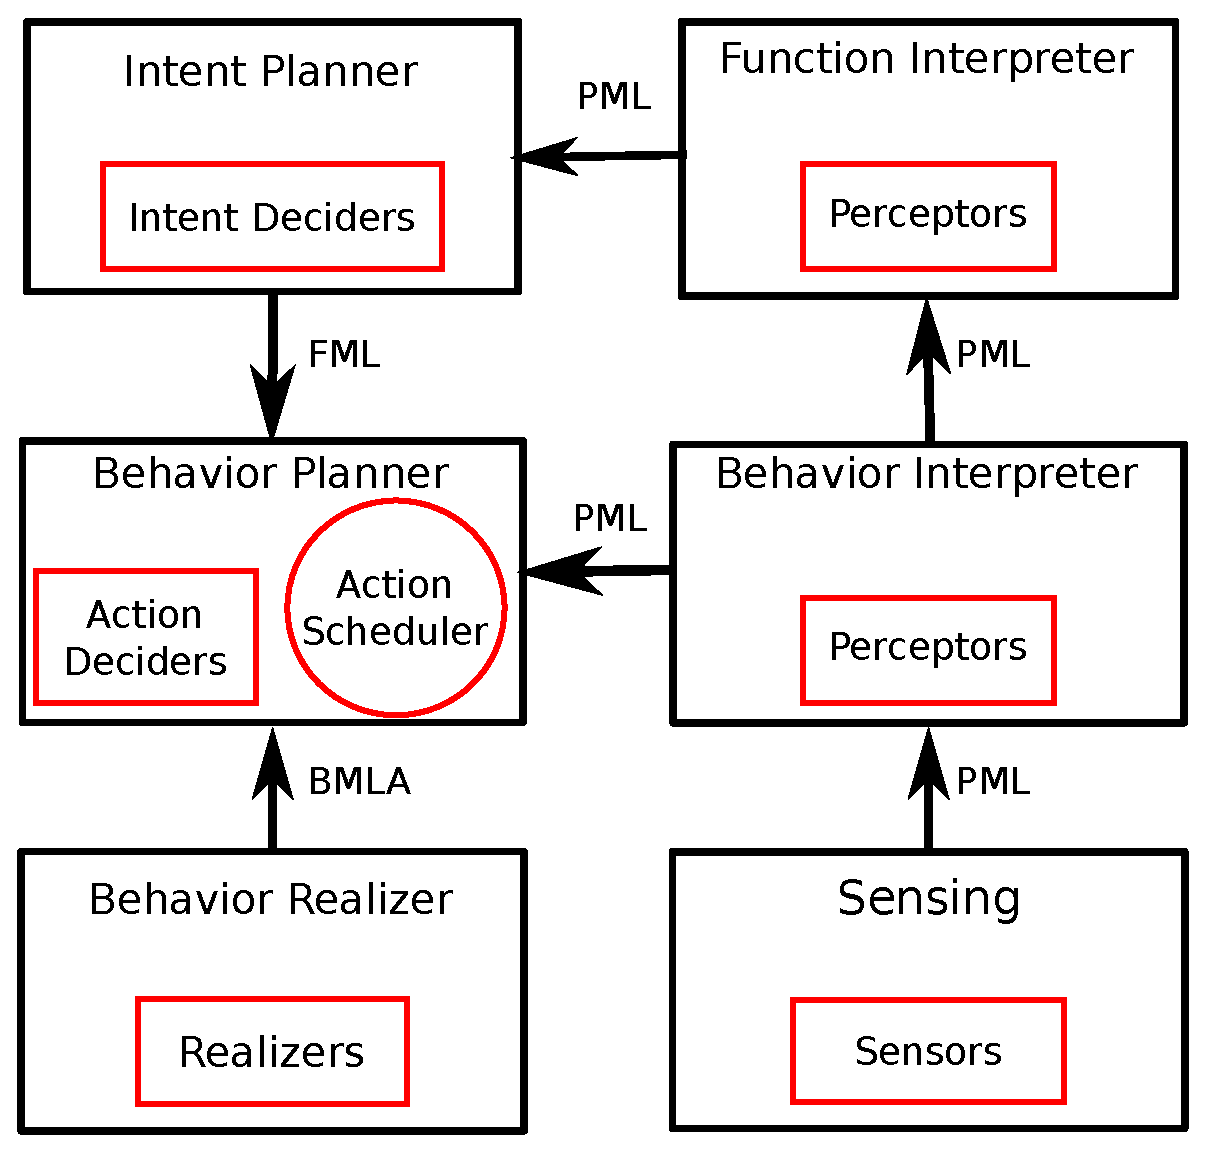
\includegraphics[width=\linewidth]{figure/impl_schema.eps}
  \caption{Overall organization of the BeAware architecture.}
  \label{overall_archi}
\end{figure}

Each module is compounded of submodules, each specialized into : \begin{itemize}
	\item the real-time acquisition of the user's verbal and non verbal signals, for submodules of the Sensing Module;
	\item into the perception of one particular behavioral pattern or communicative act, for submodules of the Behavior Interpreter and Function Interpreter;
	\item into the generation or the control of one particular communicative intention multimodal action for submodules of the Intent and Behavior Planner;
	\item into the execution of particular BML commands for submodules of the Behavior Realizer.
	\end{itemize}		
	Following the terminology of \cite{thorisson_mind_1999}, the submodules of the behavior and function interpretation modules were called perceptors, those of the Sensing modules the sensors, those of the Intent Planner and the Behavior Planner the deciders, those of the Behavior Realizer were called realizers and submodules of the sensing module were called the sensors.  
Following the Ymir principles, the different submodules run concurrently, at their own execution frequency. 
%The different execution frequencies will be defined when we will present the implementation of the model. 
Like in Ymir, the submodules can also be either activated or deactivated. 
%following \citep{thorisson_mind_1999}, defining if the submodules currently run (activated) in the architecture or not (deactivated). 
The activation or deactivation of modules depends on the current state of the dialog. 
For instance, modules implementing equations of our model controling the non verbal signals of the speaker are activated only when the agent is in the state Speaker and deactivated when the agent is in the state Listener. 
The activation or deactivation of the submodules is implemented in the Function interpreter module by so-called Module Managers. 

We distinguish two types of deciders: intention and action deciders. 
Intention deciders belong to the Intent Planner, and are responsible for the generation of the communicative intentions, based on the perception data provided by the function interpretation module. Intention deciders output FML data. 
The action deciders take as input the communicative intentions provided by the intention deciders, and the perceptual data provided by the behavior interpretation module. As output, they generate an action command that describes the action to control and the new values of the action parameters, according to the perceptual data and the agent's communicative intention. 
These commands are then sent to an action scheduler that have the responsibility to transcribe the commands into BML motor commands and to manage their concurrent executions. Once the motor commands have been determined, the action scheduler sends them to the realizers. 
The design of our action scheduler is very similar to Ymir's one. The difference is linked to the management of the continuous multimodal actions: the deciders modulating the actions of the agent, send to the action scheduler a continuous flow of commands. Our action scheduler manages this continuous flow of commands, with the capability of modifying on the fly the multimodal motor commands bound to a particular action, based on the parameters the deciders send to the action scheduler. 
Finally, the action scheduler sends the different motor commands to the corresponding realizers using BML structures. 

\subsection{Implementation}

%We now describe our we implemented the different components of our model in the architecture. We illustrate on the 

Figure \ref{impl_modules} illustrates how the different submodules are implemented in the architecture. 

\begin{figure}
  \centering
  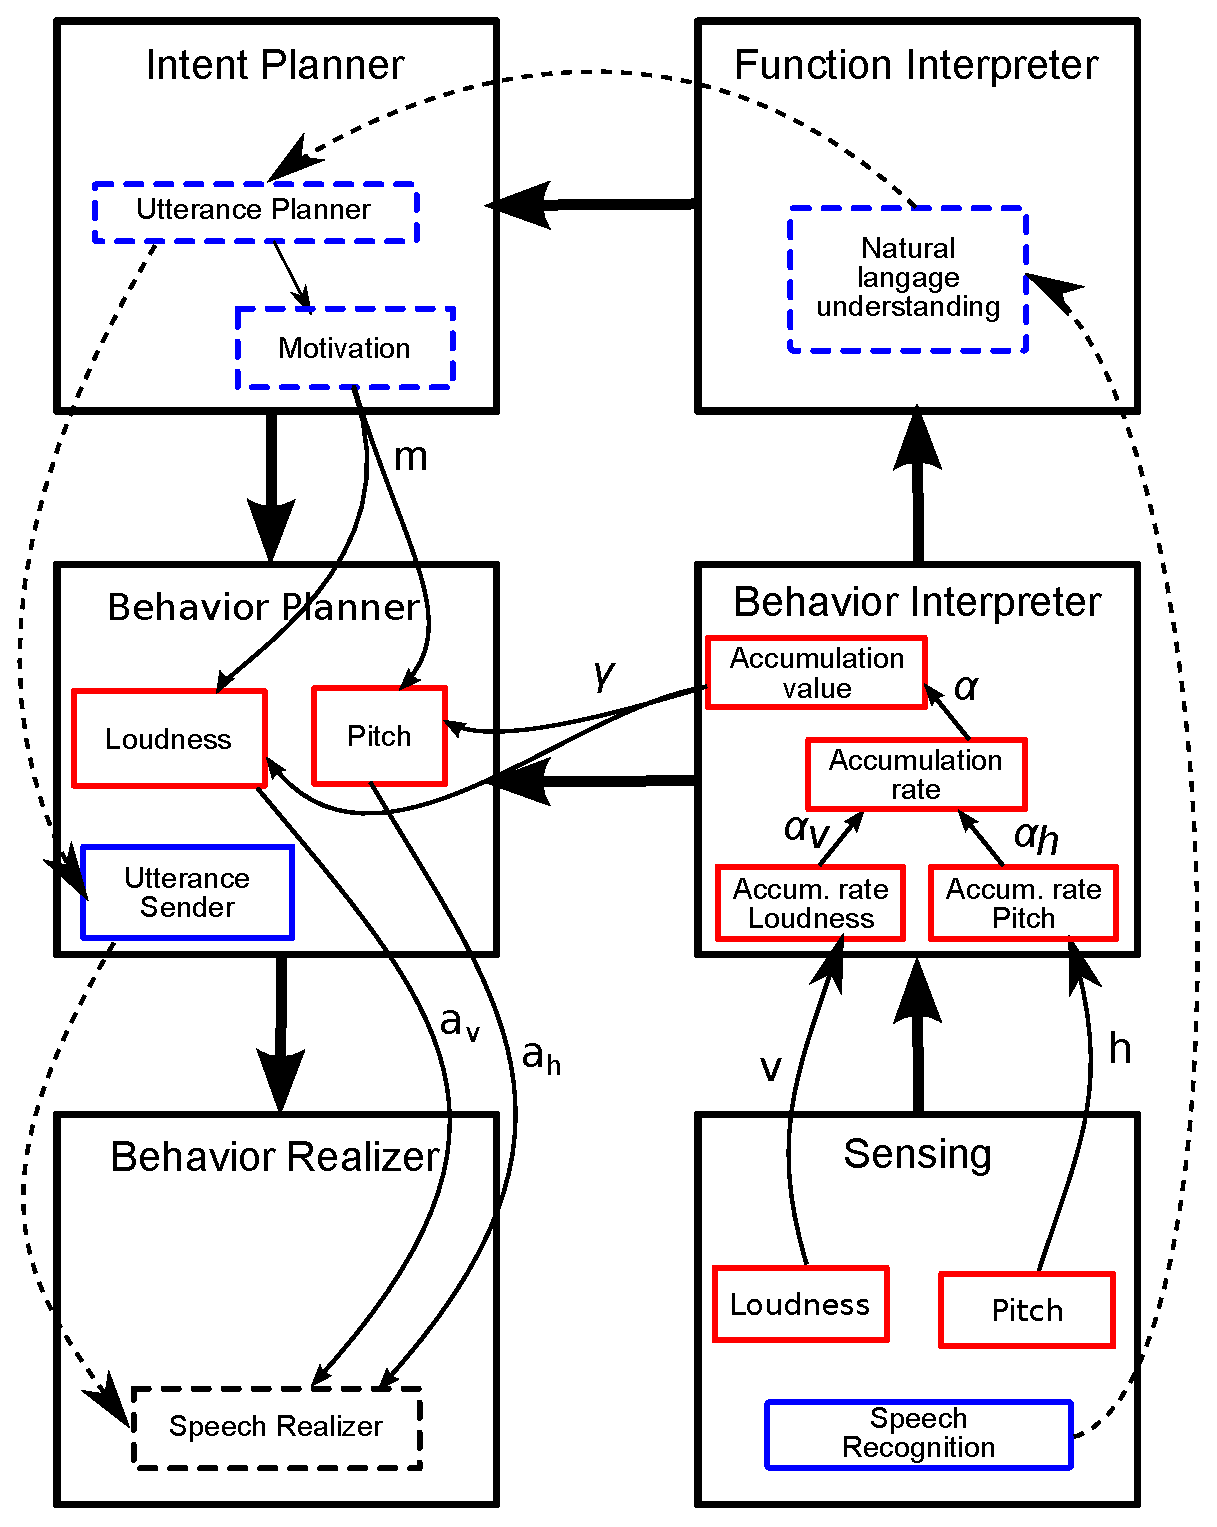
\includegraphics[width=\linewidth]{figure/impl_equ_dial.eps}
  \caption{Distribution of the components of the model and the different submodules dedicated to the utterance interpretation and generation and the determination of the motivation value.}
  \label{impl_modules}
\end{figure}

%\subsubsection{Components of the model}
\subsubsection{Perceptual decision-making process}

%The two components of our model are implemented into two different modules of the architecture. 
According to our model, the agent is continuously collecting information about the user's behavior. This is done by submodules of the Sensing Module, referred by (1) in figure \ref{impl_modules}. Two submodules are currently implemented, the Loudness and Pitch submodules that gather in real-time the loudness and pitch of the current user. 

This information is a set of characteristics computed in real-time from the data the agent is able to sense, which is used to compute the accumulation rate $\alpha(t)$. 
Each partial accumulation function $\alpha_j(t)$ is evaluated in a separate submodule (modules referred by the number (2) in figure \ref{impl_modules}). The values computed by these modules are then summed by a dedicated perceptor ((3) in figure \ref{impl_modules}), according to Equation \ref{alpha_func} and integrated by a last submodule ((4) in figure \ref{impl_modules}) which computes the final accumulation value $\gamma$ according to Equation \ref{perc_int}). The final accumulation value is then transmitted to both the Behavior Planner and the Function Interpreter. In the Function Interpreter, is implemented a submodule ((5) in figure \ref{impl_modules}) evaluating the resulting accumulation value $\gamma$ and in charge of changing the agent's current state (speaker or listener) when $\gamma$ has crossed the positive threshold $\theta_{\gamma}^{+}$. As we define different set of equations depending whether the agent is the current speaker or the current listener in our model (see section \ref{mod_pres} and \ref{mod_analysis}), the agent have different set of modules for the perception of the user's behavior and control of prosodic actions. Thus when the agent has changed state, the set of perception and control modules associated with its previous state are deactivated and the set of perception and control modules associated with its next state are activated. 

%Each signal the agent can perceived is  % produces a certain behavioral pattern that the agent has to discriminate. In this sense, 
%the user behavior perception component of our model should be implemented in the behavior interpretation module. We separate the user behavior perception component into several independant submodules. First, several submodules compute the partial accumulation rate for each signal produced by the user. These partial accumulation rates are then used by a submodule computing the global accumulation rate ($\alpha(t)$ variable in the model). This global accumulation rate is then used by the submodule in charge of updating the accumulation value according to the equation \ref{perc_int}. 
%The accumulation value is then sent to the behavior planner. 

\subsubsection{Modulation of the prosodic signals}

The corresponding components are implemented in the Behavior Planner ((6) in figure \ref{impl_modules}). In each of these modules are implemented specific equations controlling the modulation of one particular signal according, following the general shape of Equation \ref{signal_control}. Each action decider has two inputs: the motivation $m(t)$ to change role, coming from the Intent Planner and the accumulation value $\alpha(t)$, coming from the Behavior Interpreter. 
Once computed the pitch and loudness values, the deciders send these values to the action scheduler ((7) in figure \ref{impl_modules}) which is in charge to transform these command into BMLA command (an extension of BML) that are then sent to the Realizers. 
%Each signal control equation is implemented in a particular action decider, for an agent managing the pitch and loudness variations of the agent, we would have then two different deciders, one for the pitch and one for the loudness. 
%The fact that the agent can 
In our current implementation, two deciders are currently implemented, one for pitch modulation and one for loudness modulation. 
The choice of independently control the different signals may seem inconsistent especially when separately controling pitch and loudness. Indeed, when the loudness is equal to $0$, the agent does not produce any sound, talking about pitch variation does not make sense. However, the equations of our model define the control parameters of the different realizers and do not correspond to the real signal values. Potential inconsistence are then resolved later by the Realizer.  

%The management of the different physical couplings that can exist is done by the different realizers . 

\subsubsection{Management of the motivation}

The motivation to speak, or to listen, may come from different factors. If the agent is finishing its utterance and has nothing more to say its motivation to be the listener will be positive. Otherwise, its motivation will be negative. The strength of this motivation is regulated by different processes, for instance the interpersonal attitudes of the participants \citep{ter_maat_how_2010,ravenet_conversational_2015} or the importance and nature of the contribution made by the participant \citep{cafaro_effects_2016}. As the nature of the factors influencing the motivation to speak can be different, we chose to implement its computation in an independent module of the Intent planner ((8) in figure \ref{impl_modules}). This module updates over time the motivation of the agent and then sends a FML data specifying the new motivation value to the Behavior planner. 


\subsubsection{Verbal production}

In addition to the submodules implementing our turn-taking model, we added submodules dedicated to the interpretation of the user's utterances. 
User's utterance is first perceived incrementally by the Speech Recognition Module ((9) in figure \ref{impl_modules}) and then  transmitted to the Natural Language Understanding module ((10) in figure \ref{impl_modules}) that maps the user's utterance with a semantic value. This semantic value is then transmitted to the Utterance Planner ((11) in figure \ref{impl_modules}) that determine, according to this semantic value, the next utterance the agent will pronounce.  
Once the utterance is generated, it is sent to a specific submodule of the Behavior planner ((12) in figure \ref{impl_modules}). This submodule decides to send to the Action scheduler an action command specifying the utterance to say, depending on the constraint that applies to this utterance. When the communicative intention specifies that the utterance should be produced immediately, the utterance is sent directly to the action scheduler whether or not the text to speech system (TTS) is currently producing an utterance. As a result, when the speech realizer ((13) in figure \ref{impl_modules}) receives the utterance, it cancels the previous utterance and send the new utterance to the TTS. On the contrary, when the communicative intention specifies that the utterance should be generated after the current one, the decider waits until the realizer sends a feedback specifying that it has completed the production of the utterance.
As soon as the speech realizer ((13) in figure \ref{impl_modules}) receives then command specifying the generation of an utterance, it verifies the loudness and pitch values sent by the action scheduler. When the loudness value is greater than a threshold, it transmits the utterance to the TTS system. Each time the realizer receives new commands specifying the loudness and pitch values, it sends the new values to the TTS that modulates the prosody of the utterance being currently generated. When loudness value received by the realizer becomes lesser than a threshold, the realizer decides to pause the ongoing utterance production.

\subsubsection{Technical choices}

For this implementation, we focused first on the perception and modulation of the voice loudness and pitch. We defined the different equations based on observations we made on a corpus of human interactions. For more details about these equations, see \cite{jegou_continuous_2015}. For the implementation of the signal control submodules we used the Runge-Kutta 4 method and for computation of the accumulation value, the Euler-Maruyama method. 

The implementation of the architecture and the submodules has been realised in JAVA. We set the execution frequency for the different submodules to 10~Hz. 
We used openSmile \citep{eyben_recent_2013} for the captation of the user's loudness and pitch (acquisition frequency: 10 Hz). % It  mesures and sends every 100~ms the loudness and pitch value of the user. 
The agent's graphical representation and its animation have been implemented using Unity3D. 
%The character has for the moment two different animation, speaking and listening. Those animations are synchronized with the output of the TTS system, such as, when the TTS pronounce an utterance, the speak animation is played and when no utterance is pronounced the listening animation is played. 

%In order to be able to
For testing our model we needed to use incremental speech recognition and synthesis tools. Thanks to the incremental speech recognizer, the agent was able to formulate hypotheses on what the user is saying before the s/he has finished to speak. Based on the hypotheses, the agent can then plan early its own utterance and then, depending on its motivation, can choose to interrupt or not the user. For the incremental speech recognition we used the Microsoft Speech API. 
The incremental speech synthesis tools allowed to modify on the fly the properties of the utterance being pronounced by the agent, such as revising what the agent is currently saying or modulating the prosody. We mostly used an incremental speech synthesis tools to be able to modulate the prosody of the utterance pronounced by the agent. For this, we used inpro\_iSS created by \cite{baumann_inpro_2012}. 

\subsubsection{Example of interactions}

We report now four examples of real-time interactions between a user and the agent, that show the ability of the implemented model to handle non trivial situations. In the first two scenarios, the user tried to barge in the agent while the latter was uttering a long sentence (Figures \ref{sc_1} and \ref{sc_2}). In the last two scenarios (Figures \ref{sc_3} and \ref{sc_4}), the agent was answering to a user's question it had understood before the end of the user's turn. In these two scenarios, the transition of turn did not occur in the same way, depending on the agent's motivation. 
 
%In these examples, the agent was able to interpret the sentence pronounced by the user and to chose which sentence to utter in response to the user's utterance. 
For these controlled scenarios, we formulated adjacent pairs to determine which sentence the agent will say in response to the user's utterances and forced the value of the agent's motivation. 
%For each examples, we plotted the loudness profile for the interaction transcription, represented as green curves above the transcription of the dialog between the two participants. In the figures, the ``detect" annotation indicates when the agent was certain about the user's utterance and planed the utterance to be said. 

Figure \ref{sc_1} corresponds to the first interaction when the agent had a strong motivation to keep the turn ($m_{loc}=-1.0$). 
As a result, the agent raised its loudness between the expression ``mount" and ``a shelf" and the loudness remained high until the agent pronounced the word ``red". This can be explained by the accumulation variable that became positive when the user barged-in, meaning that the agent was perceiving that the user was trying to take the turn. 
%This positive accumulation value is sent from the behavior interpreter module to the behavior planner. 
Consequently, the submodules controlling the agent's actions raised up the values of their attractors, making the control parameter raising and then finally making the loudness of the utterance of the agent to raise. 
Contrarily, Figure \ref{sc_2} shows what happened when the agent had a weak motivation to keep on speaking, making it to release the turn before the end of its utterance in response to the user's signals variations.

\begin{figure}
  \centering
  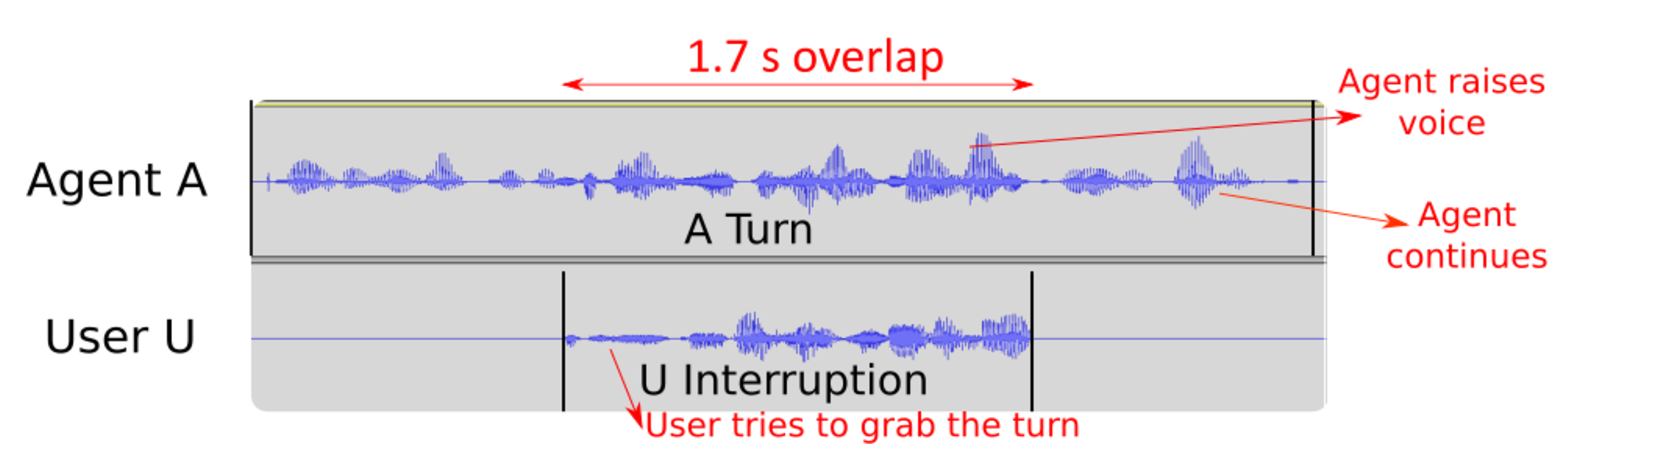
\includegraphics[width=\linewidth]{figure/volume_transcript_1_1_refait.eps}
  \caption{Illustration of the first interaction. The user tries to grab the turn, the agent raises its voice to prevent the user to interrupt then continues its turns after the user stops.}
  \label{sc_1}
\end{figure}

\begin{figure}
\centering
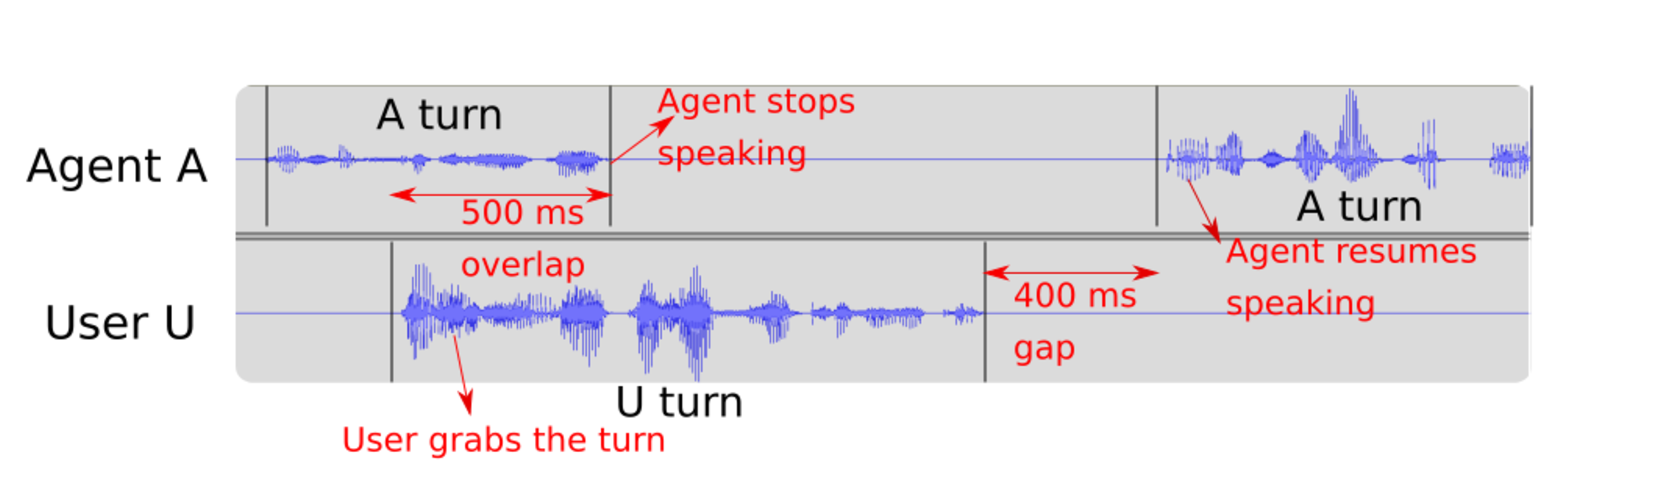
\includegraphics[width=\linewidth]{figure/volume_transcript_1_2_refait.eps}
\caption{Illustration of a scenario where the agent stops in response to the user barge-in.}
\label{sc_2}
\end{figure}

\begin{figure}
\centering
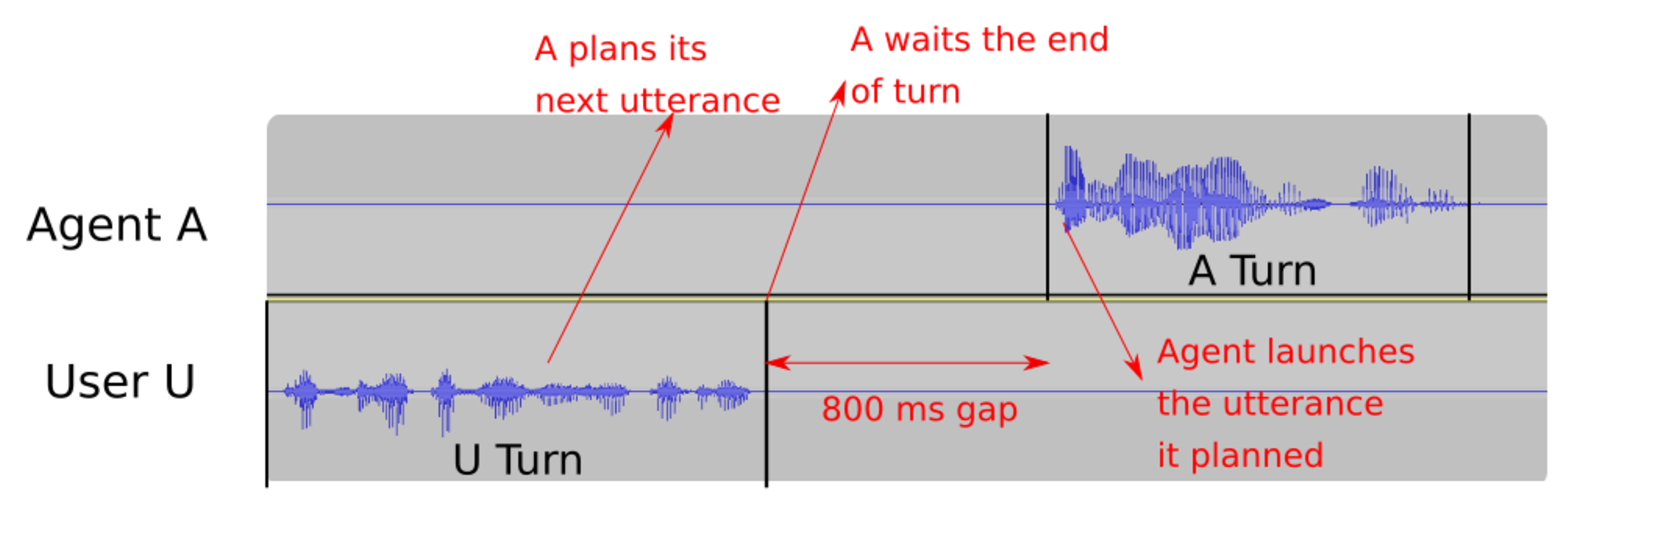
\includegraphics[width=\linewidth]{figure/volume_transcript_2_2_refait.eps}
\caption{Illustration of a scenario where the agent waits the end of turn of the user even if it has understood was the latter was saying.}
\label{sc_3}
\end{figure}

\begin{figure}
\centering
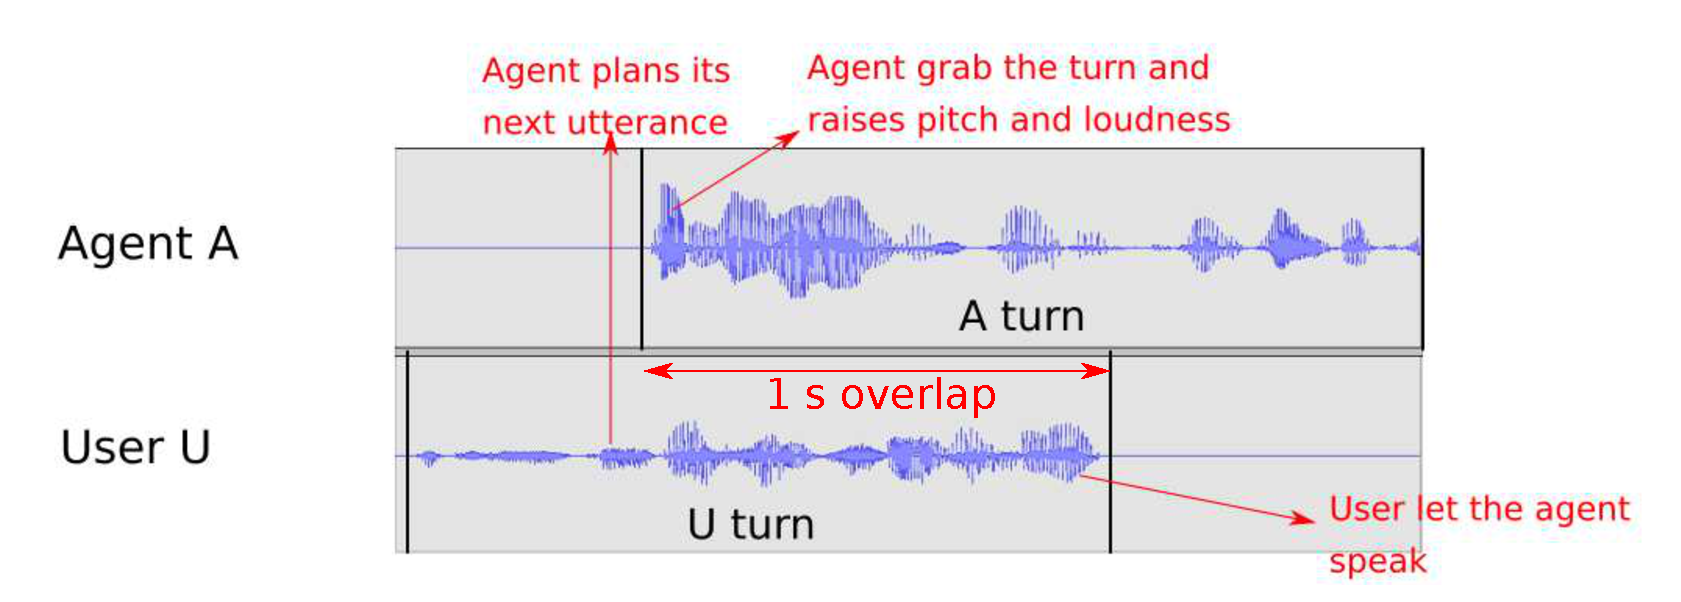
\includegraphics[width=\linewidth]{figure/volume_transcript_2_1_refait.eps}
\caption{Illustration of a scenario where the agent interrupts the user as soon as it has understood was the user was saying.}
\label{sc_4}
\end{figure}

Figure \ref{sc_3} illustrates the second interaction: the agent was the current listener and had a weak motivation to answer to the user's question, although it had understood what the user was saying before the end of the user's turn. In this situation, the agent did not start speaking before the end of the user's question. 

Figure \ref{sc_4} shows what happened in the same situation when the agent had a strong motivation to answer to the question. %shows an other example when the user asks a question to the agent, and then agent recognizes the utterance pronounced by the user before the latter has finished to pronounce it. Once the agent has recognized what the user was saying the agent wait the user finished its utterance before interrupting it. 
As soon as the agent had recognized what the user was saying, the utterance generation module planned an utterance that was sent to the realizer. Nevertheless, as the loudness command of the realizer was less than the threshold, the utterance had  not been immediately launched in the TTS. 
%The control parameter provided by the signal control submodules, the loudness parameter depends on the result of the turn-taking submodules. 
Due to its weak motivation to speak, while the user was still speaking, the loudness of the agent remained lesser than the 'silence' threshold. When the user had finished the turn, the accumulation value begun to raise towards a positive value. When this accumulation value reached a given (high) value, the loudness attractor increased, making the loudness parameter getting higher and higher. As soon as this parameter received became higher than the value of the silence threshold, the realizer launched the utterance into the TTS.
The fact the agent, in this situation, waited a while before starting to speak was due to the way we defined the loudness control equations. In these equations, depending on the motivation value, the loudness begins to raise above a positive accumulation value: the lowest the motivation, the higher the accumulation value has to be for the loudness to raise. If its motivation increases, the agent will begin to speak sooner and, as an extreme, will interrupt the user. Figure \ref{sc_4} shows that, when the agent's motivation is very strong, a long turns overlap occurs. 


\section{Evaluation of real-time interactions between the user and the agent}
\label{sec:eval}

%We present in this section an evaluation of an embodied conversational agent coordinating turns in real time with users in the context of a negociation scenario.

\subsection{Motivation}

This evaluation aimed at answering three questions: 
%\begin{enumerate}
%\item
(i) Is an agent controlled by our turn-taking model able to coordinate smoothly its speaking turns with the user?
%\item
(ii) Is an agent controlled by our turn-taking model able to correctly signal its intentions (either taking, yielding keeping or grabbing the turn) to the user?
%\item
(iii) Can an agent varying its turn-taking behavior according to our model improve judgements about the agent's credibility, user's satisfaction and easiness to interact with the agent?
%\end{enumerate}

%To that purpose we chose to inspire from 
Our methodology was based on existing evaluations techniques.
\cite{skantze_towards_2010} and \cite{de_vault_toward_2015} conducted two studies to evaluate agent's turn-taking in the context of negociation scenarios. In these two experiments, the agents were at least partially controlled by a Wizard of Oz (WOz). In \cite{skantze_towards_2010} only the user's utterances were transcribed by the WOz, the remaining being managed by the system. User's end of turns were identified using a voice activity detector and the system systematically responded to the user after detecting the end of the user's turn. In \cite{de_vault_toward_2015}, the whole process, from interpretation to generation, was managed by the Wizard of Oz, including turn-taking management. These two experiments had the advantage to answer similar research questions as ours regarding turn-taking. First, the ability of the agent to coordinate with the user was evaluated by comparisons of the agent's response time and overlap duration with human interactions. Second, the agent's credibility, the user's satisfaction and easiness to interact with the agent were evaluated through questionnaire. The ability of the agent to correctly signals its intentions towards turn-taking was not directly treated. However some behaviors of the user were analyzed in these evaluations such as the user latency to take the turn after the end of the agent's turn. To our view, these behavior could be related to the ability of the user to clearly identify signals displayed by the agent, the clearer the agent's signals, the shorter the user's response latencies. As these evaluations seemed particularly adapted to our own goals, we chose to inspire from them to elaborate our own evaluation. One major difference is that, in our case, the agent's turn-taking behaviors varied according to the output our model. 

\subsection{Protocol}

Similarly to \cite{de_vault_toward_2015} and \citep{skantze_towards_2010}, we conducted an experiment where the user was engaged in a negociation scenario with an agent. The interaction was only audio, the agent had no graphical representation and only perceived and controlled two prosodic parameters, the loudness and the pitch. 
%In the negociation scenario, both participants are on a sinking boat, and prepare to 
The scenario stages two participants on board a sinking boat, preparing to embark on a life boat. 
Each participant has different beliefs on the situation. 
One thinks that they are close to the coast, in this situation the priority is then to reach the coast as fast as possible. 
The other thinks they are far from the coast, the priority being here to survive as long as possible. 
Given their different beliefs, they have to make a share decision about three items to take away in the life boat among six. We chose the different items such as three of them were adapted to first situation 
%where participants are close to the coast 
and three to the second one.
objects were adapted to situations were participants are far from the coast. 
The scenario conducted the user, given his own belief, to disagree with the agents' proposals.   
% Déplacé en second paragraphe

We used our implementation presented in section \ref{impl}. The agent had thus a complete turn-taking module that determined when the agent utterance should be launched. In order to avoid user's utterances misinterpretations we chose to replace the Automatic Speech Recognizer and Response Planning components by a Wizard of Oz. The WOz listened and selected utterances thanks to an interface that allowed to select arguments in favor of the items the agent wanted to take and to produce counter-arguments to the user's proposals. It was necessary to avoid any influence of the Wizard of Oz response time on the agent turn-taking behavior. To that purpose, the WOz was instructed to select the agent's next utterance before the end of the user's utterance. 
To make the WOz answering as fast as possible, the interface was organised in buttons, determining the different dialog acts. Once the Wizard of Oz selected a particular dialog act by clicking the corresponding button, an utterance related to this dialog act was chosen among a list of utterances, allowing the agent to vary its answers to the user. The utterance chosen was then sent to the agent that determined when to launch the utterance according to the output of the turn-taking module, using the mechanism presented in section \ref{impl}. In order to have the most natural interactions, the different utterances that the agent could produced were collected from a corpus of human interactions we collected before. 

%À caser
%. 

% Déplacé en troisième paragraphe
%In order to assess the ability of our agent to coordinate with the user, 
We compared our turn-taking model (M1) with an implementation of a second model (M2). 
In this second model, we used a voice activity detector to discriminate moments when the user spoke from moment of silence. 
%Given the result of the voice activity detector,
The second turn-taking module was implemented following the following rules: 
\begin{itemize}
\item when no speech activity is detected after 600~ms, consider that the user has finished its turn and take the turn;
\item after at least 100~ms of speech activity, consider that the user is beginning a new turn and stop speaking. 
\end{itemize} 
These rules based on temporal threshold are often used in spoken dialog systems and agent architectures. 
Interestingly, they are considered as non-optimal \citep{ward_root_2005}. 
The two thresholds of 600~ms and 100~ms corresponded to values used in existing models (see for example \citep{ferrer_is_2002}). 

When the agent was controlled by our model M1, it was able to modulate its prosodic signals and thus to inform the user about its intentions by decreasing the pitch and loudness of its voice at the end of the turn and raising its pitch and loudness to inform the user about its intention to grab the turn.  
With model M2, the agent was not able to vary its prosodic signals and thus had no modality to convey any information about its intention. 

The values of the motivation parameter $m$ were set such as according to its current role, the agent had two possible turn-taking behavior. In the first case, the agent had a weak motivation to keep the turn as a speaker ($m=-0.4$) making it releasing the turn when it detected that the user wanted to grab the turn, and a weak motivation to take the turn as a listener making it waiting the end of the user's turn before taking the turn. In the second case, the agent had a strong motivation to keep the turn ($m=-1.0$), making it insisting to keep the turn when it detected that the user wanted to grab the turn, and a strong motivation to take the turn ($m=1.0$), making it to systematically trying to grab the turn. 

We ensured that the user interacted equally with the agent having respectively weak and strong motivation to take or keep the turn. To that purpose, we divided the interaction in two parts. In the first part the user interacted with an agent having a weak motivation to take or keep the turn, and in the second part with an agent with a strong motivation.
% the user interacted with an agent having a strong motivation to take and keep the turn. 
We kept this order for all the interactions, because beginning the interaction with an agent systematically trying to grab or to keep the turn would risk to make the user to refuse to continue to engage in the interaction with the agent. 

%As a result, we had two main conditions,
The different conditions of the experiment were as follows.
In condition 1 the user interacted with an agent controlled by model M1.
In condition 2, the user interacted with an agent controlked by model M2.
Condition 1 presented to variants, depending of the value of the motivation parameter: ``condition 1 strong'' and ``condition 1 weak''. 
% We chose to name the first part of the condition 1, when the user interacted with an agent having a weak motivation to keep and take the turn ``condition 1 weak", and the second part of the ``condition 1 strong", when the user interacted with an agent having a weak motivation to keep and take the turn ``condition 1 strong". 
Each participant interacted twice with the agent, each time with a different condition.
The order of the conditions (``condition 1" and ``condition 2") was counterbalanced between participants.
For each condition, the interaction lasted 2 min 30 s. 

At the end of each interaction, a questionnaire, presented table \ref{Answers}, was proposed to the participant, with questions about the easiness to interact with the agent (question Q9 in table \ref{Answers}), user's satisfaction (Q8, Q10) and agent credibility (Q11). The corresponding questions were adapted from \cite{skantze_towards_2010}, \cite{bevacqua_effects_2014} and \cite{de_vault_toward_2015}. Moreover, in order to assess the clarity of the agent's signals, we added questions about the intentionality of agent's interruptions that is whether interruptions of the agent were due to an agent mistakenly perceiving the end of turn of the user or where made by the agent on purpose (Q3, Q4). Finally, we added questions about the ability of the agent to smoothly coordinate with the user (Q1, Q2, Q6, Q7).
For each items, the participant had to declare its level of agreement, between strongly disagree and strongly agree in a continuous scale between 0 à 10 The different items were inspired from \cite{skantze_towards_2010}, \cite{bevacqua_effects_2014} and \cite{de_vault_toward_2015}.

\section{Results}

31 volonteers (30 men and 1 woman) participated to the experiment. They were all native French speakers and were students, engineers or researchers. The results to the questionnaire for condition 1 and condition 2 are shown on Table \ref{Answers}. 
\begin{table}
\centering
\resizebox{\linewidth}{!}{\begin{tabular}{|p{3cm}|p{2cm}|p{2cm}|p{2cm}|}
\hline
Questions & Median \linebreak conds. 1 & Median \linebreak cond. 2 & p-value \\
\hline
Q1: My interlocutor \linebreak didn't perceive the moment were I talked & 2.25 & 1.75 & 0.95\\
\hline
Q2: My interlocutor took the turn randomly& 2.5 & 2.625 & 0.6 \\
\hline
Q3: My interlocutor interrupted unvolontarily& 6 & 4 & 0.019* \\
\hline
Q4: My interlocutor interrupted me on purpose& 6 & 6.5 & 0.91 \\
\hline
Q5: My interlocutor paid attention not to interrupt me & 4.5 & 7.5 & 0.006**\\
\hline
Q6: My interlocutor was slow to respond to me & 3 & 2 & 0.77\\
\hline
Q7: My interlocutor refused sometimes to speak to me & 6.125 & 5.75 & 0.16\\
\hline
Q8: My interlocutor annoyed me by the way he took the turn & 4.5 & 3.25 & 0.54\\
\hline
Q9: I was at ease interacting with my interlocutor & 5.25 & 6.25 & 0.55\\
\hline
Q10: I liked speaking with my interlocutor & 6.625 & 7 & 0.52\\
\hline
Q11: The behavior of my interlocutor was close to the behavior of a human speaker & 5.625 & 6.5 & 0.97\\
\hline
\end{tabular}}
\caption{Mean agreements of the participants for conditions 1 and condition 2 (translated from French).}
\label{Answers}
\end{table}

%In this table are translated the different assertions of the question, the mean responses of the participants, and the significance of differences in the responses between the two conditions. 
Generally speaking, the participants liked speaking with the agent (question Q10). The results of the question related to the credibility of the agent are more mitigated (Q11), with a median value to the assertion "The behavior of my interlocutor was close to the behavior of a human speaker" of 6.5 in the second condition and 5.625 for the first condition. The users perceived that the agent paid more attention not to interrupt them (median value of 7.5 for Q5) for the second condition than for the first one. Nevertheless, participants perceived also counter-intuitively that the agent interrupted them more unvolontarily in the first condition compared to the second condition, even if the results on question Q3 did not strongly favorized this assertion (median of 6). 

\begin{figure}
\centering
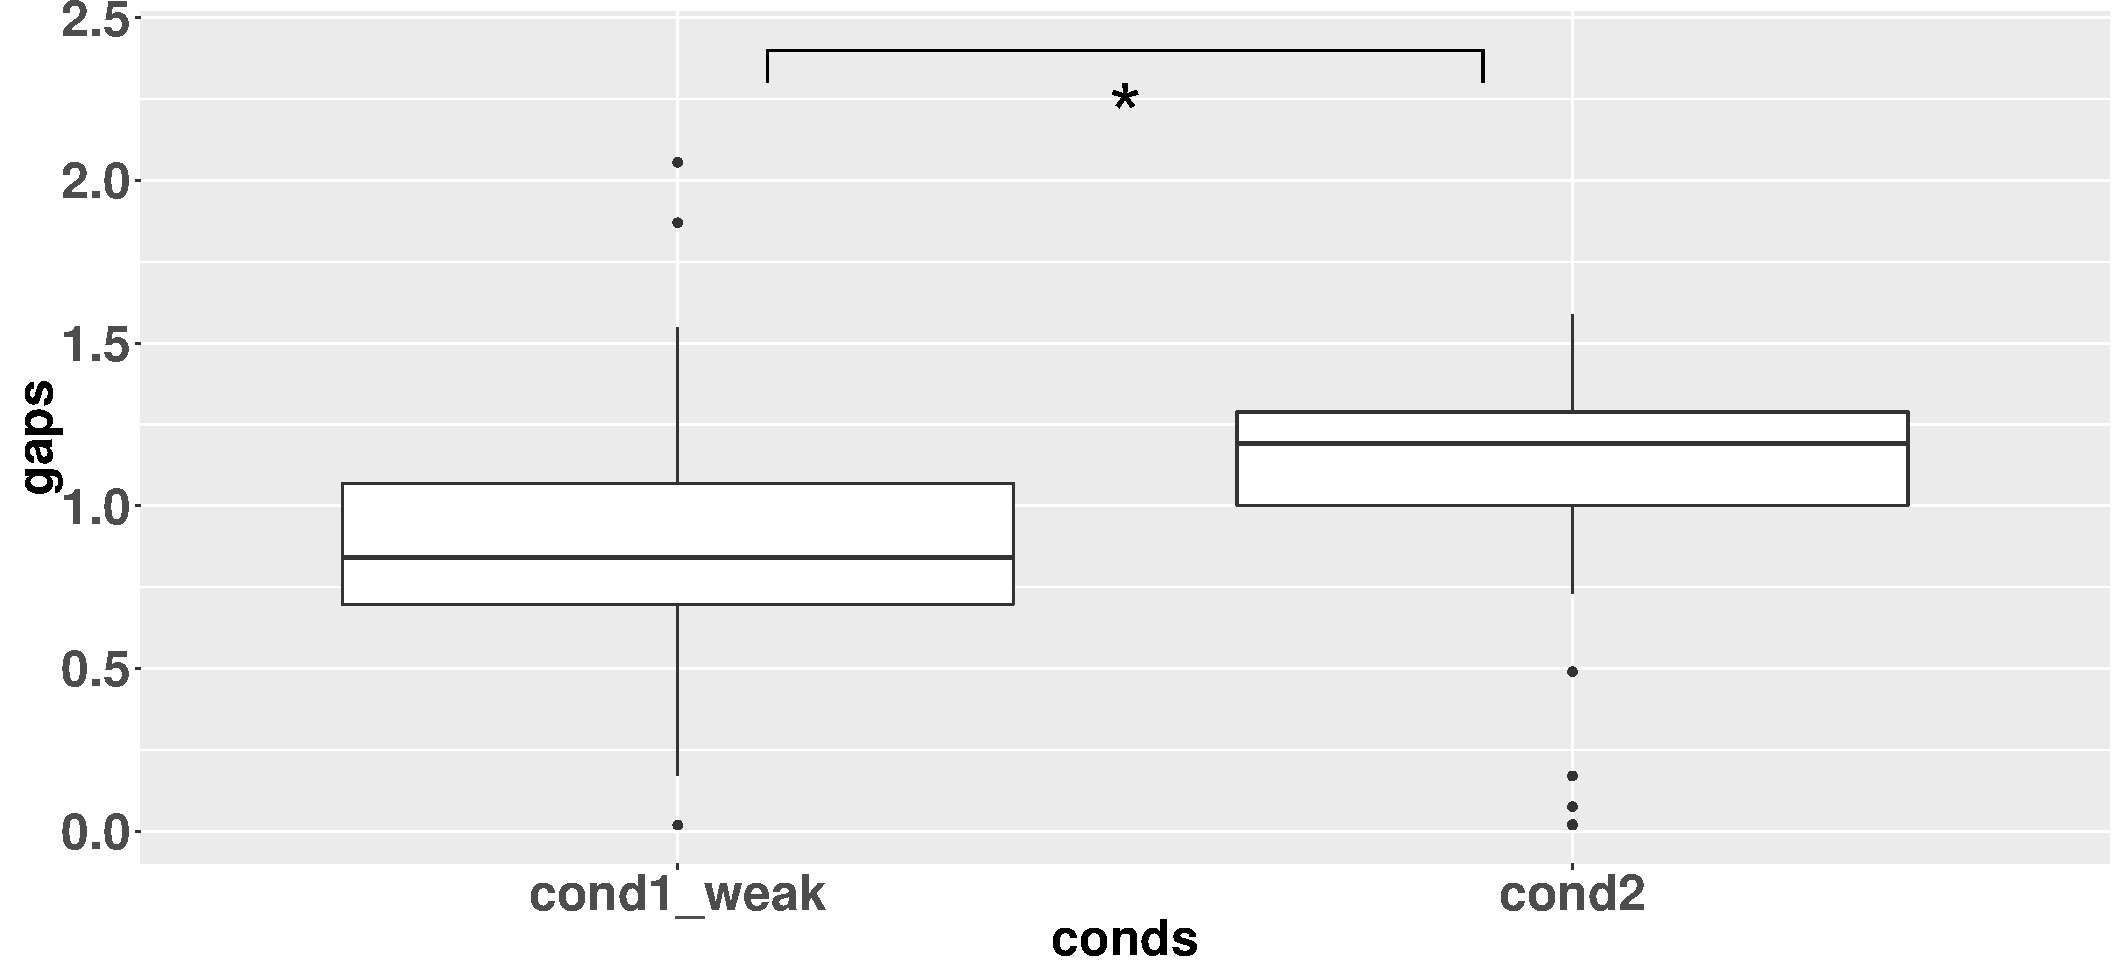
\includegraphics[width=\linewidth]{figure/boxTransitionsUA.pdf}
\caption{Durations of silence during User to Agent transitions (gaps in seconds).}
\label{box_ua}
\end{figure}

\begin{figure}
\centering
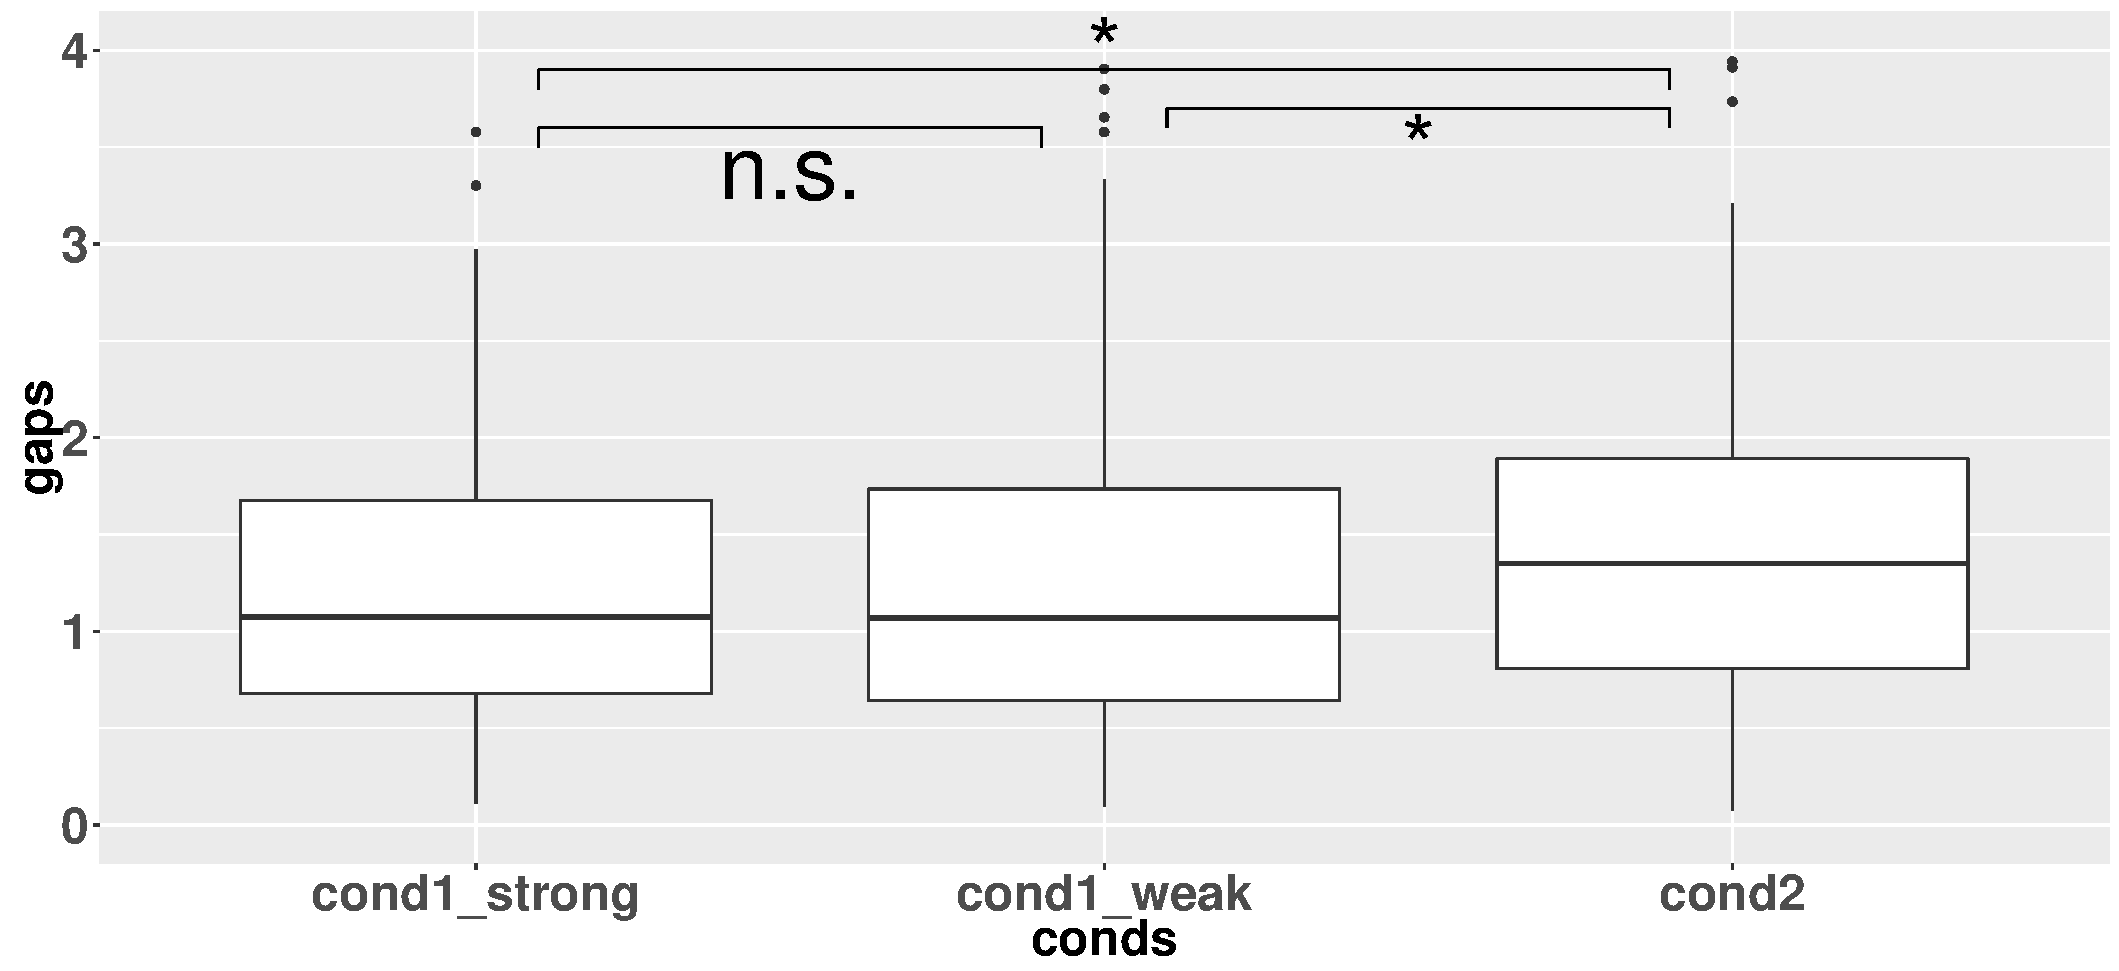
\includegraphics[width=\linewidth]{figure/boxTransitionsAU.pdf}
\caption{Durations of silence during Agent to User transitions (gaps in seconds).}
\label{box_au}
\end{figure}


We completed the analysis of the subjective evaluations with an objective analysis of the interaction. 
We first analyzed the duration of the transitions, distinguishing user to agent transitions from agent to user ones (Figures \ref{box_ua} and \ref{box_au}).
For this analysis, we annotated manually the turns of the different participants and aligned the loudness profile of the participants to the annotations we made. We kept only transitions that were not overlaps and transitions that were not anticipated by the agent. We observed first a high number of mistakes in the detection of user's end of turns, whatever the condition, with almost 50 \% of transitions having at least slight overlaps.  
%The repartition of the user to agent transitions is shown on figure \ref{box_ua}, and the repartition of agent to user transitions is shown on the figure \ref{box_au}. 

These results show that for the condition 1 the agent took the turn more rapidly (average: 840 ms) compared to the second condition (1.19 s), the difference being significant (p$<$0.05). The difference was also significant (p$<$0.05) for the agent-user transitions: in condition 1 the mean duration of silence was 1.11 s and 1.39 s for the second one. 
In addition, the pitch of the user was significantly greater than her mean pitch during conflictual moments, for condition 1 Strong. This mean that the user seemmed to react in a specific manner to the interruptions made on purpose by the agent in ``condition 1 strong". Such reaction could not be observed in the other conditions where the agent overlapped involuntarily the user's speech.
 %to these transition duration values, the pitch variation of the participants was measured during interruptions by the agent. The results showed that the pitch of the user was significantly greater than the mean pitch of the participant during conflictual moments, for the condition 1 ``Strong".

% Comment peut-on expliquer que la durée moyenne de transition soit le double du seuil de détection de la fin de tour de l'utilisateur ?
% À faire : valeur moyenne de pitch supérieure aussi lors des overlaps de l'agent pour les autres conditions, différences de perception qui pourrait laisser penser une différence de traitement ?
% Comportement de l'agent : est-ce que l'utilisateur a beaucoup interrompu l'agent ?


\subsection{Discussion}

Results show that our model improve the ability of the agent to coordinate turns with users. Indeed, while unvolontary overlaps due to mistakes in the perception of the user end of turn do not seem to differ between conditions, the agent took the turn faster in ``condition 1 weak" compared to ``condition 2". The high rate of end of turn false detections by the two models (50 \% of user-agent transitions) can be partially explained by the voice activity detector used to detect the moments were the user spoke, showing an important number of moments were no voice was detected whereas the user actually spoke. 
However, responses to questions Q1, Q2, Q6 and Q7 show that users didn't perceive this improved ability to coordinate turns. The fact that the participants seemed not disturbed by the relatively high silence duration of user to agent transitions support the idea that the latter did not expect optimal turn transitions from the agent.

Moreover, when investigating if the signals displayed by the agent were correctly perceived by the user, we observed that users considered almost equally that the agent both interrupted them unvolontarily and interrupted them on purpose both in ``condition 1" when the agent raises volume and pitch to inform the user about its intention to grab the turn and in ``condition 2" when no variation of pitch and volume are made. However, when analyzing the user's behavior, we found that the latter increased pitch when interrupted by the agent only in ``condition 1 strong". This lead us to think that users distinguish at least implicitly the volontary or unvolontary character of the interruptions and varied its reaction accordingly. This conducts us to think that solely raising pitch and loudness did not seem to sufficiently inform the agent's intention to grab the turn. The lack of distinction between interruptions, those that were due to mistakes in the detection of the user end of turn and those that were voluntary could be due to difficulties of the participants to perceive the prosodic variations of the agent. These difficulties could come from the quality of the tts voice we used, participants having often reported the bad quality of the voice. 
At the end of the experiment, we collected the oral impressions of the participants on the interaction. We also observed that participants were divided when asked about their perception of the agent's interruptions. Six participants explicitly mentionned that they perceived the interruptions of the agent as non-voluntary, on the opposite, thirteen participants perceived at least some interruptions as voluntary. 

We also analyzed the way the agent signals at the end of turn helped users coordinate with the agent. As a result, we found that users took the turn faster after the end of the agent's turn in ``condition 1" compared to ``condition 2". Two hypotheses can be made to explain this variation in behavior. First, the user could have perceived the decrease in pitch and loudness made by the agent to inform its intention to release the turn, this perception helping the user to identify the agent's end of turn. Second, variations in agent-user transition durations could be the result of an alignment effect: the fact that the agent took the turn faster made the user take the turn faster. This hypothesis is plausible, as such alignment has been observed in human conversations \citep{levitan_entrainment_2015}.  

Finally, the results of our questionnaire do not permit to conclude about the effect of varying turn-taking behaviors to the user's judgements about the agent's credibility, user's satisfaction and easiness to interact with the agent, as answers to questions Q8, Q9, Q10 and Q11 are not significantly higher for condition 1 compared to condition 2. Moreover, answers to these questions do not strongly favorize positive impressions about the agent. However, oral impressions collected after the interaction are not so categorical.   
For example, perception of the interruption seems to conduct to more positive impressions about the interaction for some participants. Four participants judged interruptions as coherent and credible given the dialog context, and five participants associated these interruptions to the fact that the agent did not agree or tried to impose its own ideas. Finally, among those thirteen participants, five participants judged those interruptions as humanlike. On the oppoposite, one of the participants we interviewed after the experiment reported a rage feeling linked to the incessant interruptions of the agent, and two participants reported that they were annoyed by these interruptions. We could explain differences in the impressions given by interruptions by the fact that the agent interrupted the user regardless of the dialog context. This could results in moments where the agent's interruptions seemed not credible given the dialog context while other interruptions were particularly relevant given the dialog context. Interruptions could thus give an impression of smoothness and immersion in the dialogue to the condition that they should be made coherently with the dialog context. 





\section{Conclusion}

\subsection{Contribution of this article}

We presented three different contributions in this article. First, we elaborated a theoretical model for the coordination of turn between the user and the agent. Our assumption is that the coordination of turns is partly an emergent property that comes from the sensorimotor coupling between the participants. 
%We simulated the model in the context of theoretical agent-agent simulations. 
%We showed in this context the capacity of our agents to coordinate their speaking turns and we reproduces qualitatively the situations observed in human interactions. 
The agents controlled by our theoretical model are adaptative, they are able to ensure a coordination in different types of environment and in interactions with partners that have more or less inertia in producing their signals or perceive more or less rapidly the behavior of their partner. Even if we presented only two types of adaptation, to the absence of presence of signals and to the way the user produces its signals, these simulations show the capability of an emergent model to reproduce the situations linked to the coordination of turns observed in human conversations.

This adaptatibility is essential as there exists a variability in the way the users coordinate their turns with the agent. This adaptation mecanism is based on the idea that the participants modify the way they produce their signals in order to keep the coordination effective. This principle is interesting because it highlights the fact that, not only the agent must be able to perceive reliably the user's intentions, but the latter has also to perceive reliably the agent's behavior in different environmnental settings. One way to guaranty that the user still perceive reliably the agent's behavior is that the agent adapts its behavior to clarify its intentions to the user, capacity that we observed in our theoretical simulations without needing to modify the equation controling the signal productions. This view of user-agent adaptation is also new in the context turn-taking, as past approaches relied on offline machine learning techniques or online reinforcement learning to perceive reliably the behavior of the user, without taking into account the way the user perceives the agent's behavior. 
However, aplying this principle of adaptation requires also the ability of the user to adapt his signals production in order to clarify his behavior and intentions. Whether the user could adapt his behavior to the agent and environment is currently a research questions, and needs further analyses of user-agent interactions to answer this question. Some clues let us think that a kind of adaptation of the user to the agent is done, as we observed a variability in the silence durations after the end of the agent's turn and before the user's beginning of turn whether the user interacted with the agent controlled by our model or interacted with the agent controlled by a model based on temporal thresholds. Nevertheless, we do not know the exact reason of this variability, it could be due to the prosodic signals produced by the agent at the end of its turn or linked to a temporal alignment of the user to the way the agent takes the turn, a phenomenon that is observed in conversations. 

% ---
As a second contribution, we presented an architecture for the implementation of both continuous and discrete control models of the agent's behavior. Our model distinguish from traditional evenemential, purely reactive models and rather is based on a continuous perception of the user's behavioral cues and a continuous modulation of the agent's actions. Few actual embodied conversational agents permit to implement these types of models. In order to integrate our model in a embodied conversational agent architecture we extended the actual ASAP architecture \cite{kopp_architecture_2014} with different principles inspired from the Ymir architecture \citep{thorisson_mind_1999}. By extending ASAP compliant with the current SAIBA standard, we made our model integrable with existing modules, managing other aspects of user-agent interactions, such as verbal interaction, emotions or interpersonal attitudes or realizers managing gestures or the gaze direction of the agent. As a demonstration, we showed the capability of an agent controlled by our model to manage turns in real-time dialogical interactions with users, and showed that in some ways, our model work with real-time user-agent behaviors. 

Finally, we analyzed real-time interactions between user and agent. Our aim was to complement actual perceptual studies about the user's experience with an agent modulating its turns, and verifying the effectiveness of the coordination between several interactions with different users. We then measured factors related to the credibility of the agent, its social presence, the satisfaction and easiness the user interacted with the agent.  We did not observe differences in the answers of the participants to the questions about those factors. We also found that participant did not always perceived the interruption of the agent as voluntary, and we found that the agent had troubles sometimes coordinating with the user. Different elements can be improved to improve the interaction between the user and the agent. First, the unvolontary and voluntary aspect of the interruptions are likely to be linked with the verbal content of the agent's utterance, and maybe there need to be a particular way to formulate the utterance when interrupting the user. It would then necessitates an extension of our actual model, linked to the management of the verbal content linked to turn-taking. Second, the agent only interacts with the user by interpreting and modulating prosody, adding multimodal interpretation abilities could certainly improve the way the agent coordinates with the user. Also for this implementation, since we determined manually the parameters of the agent's equations, optimizing these parameters could improve the coordination between the user and the agent. 

\subsection{Future work}

In the future, we plan to explore more in details the different mecanism of alignment linked to the coordination of turns as highlighted by authors \citep{benus_pragmatic_2011}, we wish to show that our current model could account for the temporal alignment we can observe in human conversations.  

As we mentioned in section \ref{backgd}, a complete turn-taking model makes intervene several cognitive process, from sensorimotor coupling to projection, and in order to have a complete turn-taking model, we need to take into account all these processes. One of the major question regarding these process in how verbal content interpretation should be done by an agent. To adress this question, \cite{de_vault_incremental_2011} proposed a statistical model where the following sentence and the content is predicted by the agent. This method could work in real-time interactions when the agent the dialog domain is well determined but as the dialog capacities and the set of utterance the user could say increases this method could become rapdily fastidious or even impossible to perform by an agent. 
As mentionned in section \ref{backgd}, verbal content is however one of the mostly used signals for the listener to detect end of turn \cite{de_ruiter_projecting_2006}, and should considerably help participants to coordinate the speaking turns. Nevertheless, the way we could implement the interpretation mecanism in an embodied conversational agents remains unclear, firstly because the process used by human participants to coordinate turns based on verbal informations is still debated \citep{heldner_pauses_2010,magyari_prediction_2012,riest_anticipation_2015}. Secondly, because the way hypothesized by a majority of authors implies perceiving reliably word by word the utterance said by the user and be able to perceive and reason about the syntax of the utterance in real-time \citep{sacks_simplest_1974}, capacities that current natural language understanding components barely have currently. 
Other extension possibility is linked to the management of speaking turns in multiparty interactions. Such models makes intervene other issues like addressing its utterance to one or a subset of participants and for as listener detecting the role its has in conversations (addressee, bystander, overhearer), managing conflicts between several previous listeners trying to take the turn at the same time. These issues are linked to a more complex management of gaze direction, the management of the participants locations. 
Moreover, our model makes intervene a motivation to change role and a motivation to keep role. Usually in human conversation, when participants are motivated to be and stay listeners, they produce backchannel in order to show the current speaker they still listen what he is saying. Thus, in our model, we could exploit this motivation to keep the agent's role to implement some behaviors related to grounding such as backchannels. For the speaker, interpreting a backchannel at some moments in time could impact the perception of the user's behavior related to turn-taking as a user producing backchannel likely won't change role immediately.

% 

\bibliographystyle{spmpsci}

\bibliography{jmui}

\end{document}